% =====================================================================
%  Bachelorarbeit CBS_MARLon
%  Einfluss der Netzwerktopologie auf die Lerneffizienz eines
%  RL-basierten Verteidigungsagenten in simulierten Cyberangriffs-
%  szenarien.
%
%  Dokumentklasse: htwg-report (HTWG Corporate Identity)
%  Quelle: https://github.com/FunkeMT/htwg-latex  (MIT, siehe
%  LICENSE-htwg-template). Die Klasse liegt bewusst im Projekt, weil sie
%  nicht ueber CTAN verfuegbar ist. Eine Abweichung vom Original ist im
%  cls-File markiert (Zitierstil numerisch statt alphabetisch).
%
%  Kompilieren:  .\build.bat   (pdflatex + biber, kein Perl noetig)
%  WICHTIG: thesis.pdf vorher im PDF-Viewer schliessen, sonst schlaegt
%  der Build mit "I can't write on file thesis.pdf" fehl.
% =====================================================================
% oneside: einseitiger Satz. Ohne diese Option erbt die Klasse den
% zweiseitigen Modus von "book"; Kapitel begaennen dann stets auf einer
% rechten Seite und LaTeX schoebe dafuer Leerseiten ein. Die Option wird
% von der Klasse an book durchgereicht (\DeclareOption*).
% Fuer beidseitigen Druck einfach "oneside" entfernen.
\documentclass[german,oneside]{htwg-report}

% ── Kodierung und Schrift ────────────────────────────────────────────
% Die Klasse laedt babel, setspace, amsmath, caption, xcolor, tikz,
% listings, geometry, hyperref und biblatex bereits selbst.
\usepackage[T1]{fontenc}
\usepackage[utf8]{inputenc}
\usepackage{microtype}
\onehalfspacing            % 1,5-zeilig (typisch fuer Abschlussarbeiten)

% Absaetze durch vertikalen Abstand statt durch Erstzeileneinzug trennen.
% parskip setzt \parindent auf 0 und \parskip auf einen passenden Wert.
\usepackage{parskip}

% ── Mathematik & Zahlenformat ────────────────────────────────────────
\usepackage{siunitx}
\sisetup{output-decimal-marker={,}, group-separator={.}}  % dt. Zahlenformat

% ── Grafiken und Tabellen ────────────────────────────────────────────
\usepackage{graphicx}
\graphicspath{{abbildungen/}}
\usepackage{booktabs}
\usepackage{tabularx}
% longtable: Tabellen, die an ihrer Stelle im Text stehen bleiben (kein Float),
% aber ueber Seiten hinweg umbrechen duerfen. Genutzt von den Reward-Tabellen in
% Kapitel 3, die sonst als unteilbarer Block eine halbe Seite frei lassen.
% Die X-Spalte von tabularx ist dort nicht verwendbar: longtable ermittelt seine
% Spaltenbreiten in einem eigenen Durchlauf, was die Ausrichtung zerstoert.
% Deshalb feste Breiten, hier einmal definiert.
\usepackage{longtable}
% Spalten der Reward-Tabellen: Ereignis, Reward (rechtsbuendig), Anmerkung.
% Bewusst OHNE @{} an den Aussenkanten: colortbl zeichnet die grauen
% Zeilenbaender stets um \tabcolsep breiter als die Spalten. Schneidet man den
% aeusseren \tabcolsep mit @{} weg, stehen die Baender ueber die Striche von
% booktabs hinaus. Behaelt man ihn, decken sich Baender und Striche genau.
% Die Breiten sind entsprechend so gewaehlt, dass Spalten plus \tabcolsep
% zusammen die Textbreite ergeben.
\newcolumntype{E}{>{\raggedright\arraybackslash}p{0.24\textwidth}}
\newcolumntype{W}{>{\raggedleft\arraybackslash}p{0.26\textwidth}}
\newcolumntype{K}{>{\raggedright\arraybackslash}p{0.41\textwidth}}
\usepackage{subcaption}
\usepackage{adjustbox}     % max width fuer die Topologie-Abbildungen
% float stellt [H] bereit: Abbildung bleibt exakt an der Stelle im Text, an der
% sie steht. Noetig, weil die Topologie-Abbildungen unmittelbar zu dem Absatz
% gehoeren, der sie beschreibt, und als Gleitobjekte sonst dazwischenrutschen.
\usepackage{float}

% ── Farben (Ergaenzung zur CI-Palette der Klasse) ────────────────────
\definecolor{navy}{HTML}{1E2761}

% \diag: hebt in den Matrizen aus Kapitel 4 die Zellen hervor, in denen
% verteidigte Topologie und Trainingstopologie des Angreifers uebereinstimmen.
% Hintergrundton plus Fettung, weil die Zeilen der Klasse ohnehin abwechselnd
% grau hinterlegt sind und eine reine Fettung dort untergeht.
\newcommand{\diag}[1]{\cellcolor{htwg-teal!18}\textbf{#1}}

% \offen: gelb hinterlegte Stelle, an der noch etwas zu klaeren ist.
% VOR DER ABGABE ENTFERNEN -- entweder den Aufruf aufloesen oder die
% Definition auf \newcommand{\offen}[1]{#1} setzen, dann bleibt der Text
% unveraendert und nur die Farbe verschwindet.
% soul statt colorbox: eine colorbox ist ein unteilbarer Kasten und schiebt
% laengere Stellen auf die naechste Seite; \hl bricht mit dem Text um.
% Der markierte Text darf dafuer keine Makros und keine Mathematik enthalten.
\usepackage{soul}
\newcommand{\offen}[1]{{\sethlcolor{yellow}\hl{#1}}}

% Nummerierung bis zur subsubsection. Ohne das erhaelt eine subsubsection
% keine eigene Nummer, ein \label dahinter uebernimmt den zuletzt gesetzten
% Zaehler (etwa eine Tabellenunterschrift), und der Querverweis springt an
% die falsche Stelle. Das Inhaltsverzeichnis bleibt unveraendert, weil
% tocdepth beim Klassenstandard 2 bleibt.
\setcounter{secnumdepth}{3}

% ── TikZ-Stile der Topologie-Abbildungen ─────────────────────────────
% Die Abbildungen selbst werden von abbildungen/gen_topologie_figuren.py
% aus thesis_topology/ erzeugt und nicht von Hand gepflegt.
% =====================================================================
%  TikZ-Stile fuer die Topologie-Abbildungen (Kapitel 2).
%  Wird einmal in der Praeambel von thesis.tex geladen.
%  Die Abbildungen selbst erzeugt abbildungen/gen_topologie_figuren.py.
% =====================================================================
\usetikzlibrary{arrows.meta, positioning, fit, backgrounds}

\definecolor{topoNode}{HTML}{E8EDF2}   % neutrale Knoten
\definecolor{topoLine}{HTML}{5A6672}   % Rahmen und Erreichbarkeitskanten
\definecolor{topoEntry}{HTML}{FFE0B2}  % Einstiegsknoten
\definecolor{topoCJ}{HTML}{F8C9C4}     % Crown Jewel
\definecolor{topoDC}{HTML}{D6E4F0}     % Domain Controller
\definecolor{topoCred}{HTML}{B03A2E}   % Credential-Kanten

\tikzset{
  topofig/.style={
    every node/.append style={font=\scriptsize},
    >={Stealth[length=4pt]},
  },
  netnode/.style={
    draw=topoLine, line width=0.4pt, fill=topoNode, rounded corners=2pt,
    align=center, inner sep=2.5pt, minimum width=17mm, minimum height=7mm,
  },
  entrynode/.style={netnode, fill=topoEntry, line width=0.8pt},
  cjnode/.style={netnode, fill=topoCJ, line width=0.8pt},
  dcnode/.style={netnode, fill=topoDC},
  % Strukturell nie erreichbare Knoten: blass und gestrichelt umrandet.
  isolated/.style={draw=topoLine!55, dashed, fill=topoNode!45, text=black!55},
  reach/.style={draw=topoLine, line width=0.5pt, ->},
  cred/.style={draw=topoCred, line width=0.5pt, densely dashed, ->},
  dcbadge/.style={font=\tiny\itshape, text=topoLine, inner sep=1pt},
}

% Legende, damit sie nicht in jeder Abbildung wiederholt werden muss.
\newcommand{\topolegende}{%
  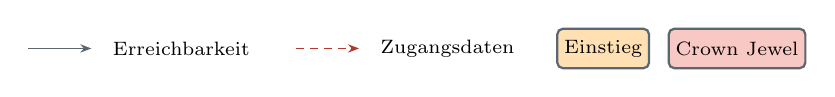
\begin{tikzpicture}[topofig, baseline]
    \draw[reach] (0,0) -- (0.8,0);
    \node[anchor=west, font=\scriptsize] at (0.95,0) {Erreichbarkeit};
    \draw[cred] (3.4,0) -- (4.2,0);
    \node[anchor=west, font=\scriptsize] at (4.35,0) {Zugangsdaten};
    \node[entrynode, minimum width=11mm, minimum height=5mm] at (7.3,0) {Einstieg};
    \node[cjnode, minimum width=11mm, minimum height=5mm] at (9.0,0) {Crown Jewel};
  \end{tikzpicture}%
}


% ── Code-Listings ────────────────────────────────────────────────────
\lstset{
  basicstyle=\ttfamily\small,
  breaklines=true,
  frame=single,
  numbers=left,
  numberstyle=\tiny\color{gray},
  keywordstyle=\color{navy},
  captionpos=b,
}

% ── Literatur ────────────────────────────────────────────────────────
\addbibresource{literatur.bib}

% ── Abkuerzungen und Querverweise ────────────────────────────────────
% acronym nach hyperref (aus der Klasse), aber VOR cleveref laden.
% nohyperlinks + diese Reihenfolge vermeiden die acronym/cleveref-
% Kollision (undefinierte Hyper-Refs, mehrfach definiertes Label 'a').
\usepackage[nohyperlinks]{acronym}
\usepackage[ngerman]{cleveref}

% =====================================================================
%  METADATEN - hier und NUR hier alle Angaben pflegen.
%  Cover und Titelblatt ziehen sich alles von hier; frontmatter/
%  titelseite.tex muss nicht mehr angefasst werden.
% =====================================================================
\newcommand{\arbeitstitel}{Einfluss der Netzwerktopologie auf Reinforcement-Learning-basierte Verteidigungsagenten in simulierten Cyberangriffsszenarien}
% Ohne \textsc: Kapitaelchen wirken in der serifenlosen CI-Schrift wie ein
% Schriftwechsel, weil helvet keine echten Kapitaelchen hat und LaTeX sie
% durch verkleinerte Grossbuchstaben ersetzt.
\newcommand{\autorname}{Mika Oelhoff}
\newcommand{\studiengang}{Wirtschaftsinformatik}
\newcommand{\erstgutachter}{Prof.\ Dr.\ Bohnet}
\newcommand{\zweitgutachter}{Prof.\ Dr.\ Langweg}

% Abgabedatum: \today setzt automatisch den Tag des Kompilierens.
% VOR DER ABGABE durch das feste Datum ersetzen, z.B. {15.\,September 2026}.
% Sonst steht auf dem gedruckten Exemplar das Datum des letzten Builds.
\newcommand{\abgabedatum}{31. August 2026}

% Angaben fuer Cover und Titelblatt der htwg-report-Klasse
\reporttype{bachelor}                 % steuert die B-S-C-Elemente des Covers
\reporttypetext{Bachelorarbeit}
\title[Einfluss der Netzwerktopologie auf Verteidigungsagenten]{\arbeitstitel}
\author{\autorname}
\studentnumber{304572}
\studentemail{[mika.oelhoff@htwg-konstanz.de]}
\doclocation{Konstanz}
% \docdate speist NUR die Ortszeile auf dem Cover ("Konstanz, <Datum>").
% Bewusst \today: waehrend des Schreibens sieht man auf dem Deckblatt,
% wie aktuell ein Ausdruck ist. Das feste Abgabedatum steht auf dem
% Titelblatt und kommt aus \abgabedatum.
% Fuer die Abgabe ggf. auch hier auf \abgabedatum umstellen.
\docdate{\today}

\hypersetup{
  pdftitle={\arbeitstitel},
  pdfauthor={\autorname},
}

% =====================================================================
\begin{document}
\frenchspacing

% ── Titelei (roemische Seitenzahlen) ─────────────────────────────────
\frontmatter

\makecover[]

\begin{titlepage}
\newgeometry{hscale=0.81,vscale=0.8}

% Kein Erstzeileneinzug auf dem Titelblatt. Sonst ruecken nur die ERSTEN
% Zeilen der Absaetze ein und Umbruchzeilen wie "Fakultaet Informatik"
% stehen buendig links, was unsauber aussieht.
\setlength{\parindent}{0pt}

\AddToShipoutPicture*{\BackgroundImgTitelPage}

\vspace*{12\bigskipamount}

%% Titelblock in HTWG-Petrol auf weissem Grund.
{\makeatletter
\fboxsep=0pt
\colorbox{htwg-white}{\begin{minipage}[t]{145mm}
    \begin{flushleft}
        \color{htwg-teal}\Huge{\@report@typetext}
        \\
        \color{htwg-teal}\Huge\textbf{\@title}
    \end{flushleft}
\end{minipage}}
\makeatother}

\bigskip
\bigskip

vorgelegt von

\bigskip

{\makeatletter
\Large\bfseries\@author
\makeatother}

\vfill

zur Erlangung des akademischen Grades

\bigskip

{\bfseries Bachelor of Science}

im Studiengang \studiengang

\bigskip

an der Hochschule Konstanz Technik, Wirtschaft und Gestaltung,\\
Fakultät Informatik

\vfill

\begingroup
\renewcommand*{\arraystretch}{1}
\rowcolors{2}{white}{white}
{\makeatletter
\begin{tabular}{@{}ll}
    Matrikelnummer:      & \@student@number \\ \\
    Abgabedatum:         & \abgabedatum \\ \\
    Erstgutachter\slash in:  & \textbf{\erstgutachter} \\
    Zweitgutachter\slash in: & \textbf{\zweitgutachter}
\end{tabular}
\makeatother}
\endgroup

%% Seitenraender wieder auf den Satzspiegel des Fliesstexts zuruecksetzen.
\newgeometry{hscale=0.7,vscale=0.8}
\end{titlepage}


% Kurzfassung (Deutsch) und Abstract (Englisch)
\chapter*{Kurzfassung}
\addcontentsline{toc}{chapter}{Kurzfassung}

Reinforcement Learning wird zunehmend für autonome Cyberabwehr erprobt;
welche Rolle die Struktur des verteidigten Netzes dabei spielt, ist jedoch
wenig untersucht. Diese Arbeit misst den Einfluss der Netzwerktopologie
auf Verteidigungsagenten, die mit Proximal Policy Optimization in der
Simulationsumgebung CyberBattleSim trainiert werden, erweitert um einen
lernenden Verteidiger. Auf vier Topologien mit identischem
Inventar -- vollvermascht, Hub-and-Spoke, DMZ und mikrosegmentiert --
treten je sechs eingefrorene Angreifer an: fünf Spezialisten und ein über
alle Topologien gestuft trainierter Generalist. Die Datengrundlage bilden
120 Trainingsläufe über fünf Zufallsstartwerte sowie eine Evaluation mit
9000 Episoden gegen drei Vergleichsstufen. Ein Einfluss der Topologie auf
die Lerngeschwindigkeit ließ sich nicht nachweisen; auf das erreichte
Ergebnis ist er hingegen deutlich: Mit zunehmender Segmentierung sinkt der
Anteil der Episoden, in denen der Angreifer das wertvollste System
erreicht -- im mikrosegmentierten Netz bis auf null, während er im
vollvermaschten Netz nahezu ungebremst bleibt, weil Sperren dort
ausweichbar sind; erst Engpässe machen sie wirksam. Der auf der
verteidigten Topologie trainierte Angreifer erweist sich durchweg als
härtester Gegner. Methodisch zeigt die Arbeit, dass der Reward allein
Verteidigungsleistung nicht abbildet und das übernommene Reward-Design
Prävention unsichtbar ließ. Für die Praxis stützt das die Empfehlung
konsequenter Segmentierung: Sie begrenzt, was ein Angreifer erreichen
kann, und macht aktive Verteidigung erst wirksam.

\chapter*{Abstract}
\addcontentsline{toc}{chapter}{Abstract}

Reinforcement learning is increasingly explored for autonomous cyber
defense, yet the role played by the structure of the defended network has
received little attention. This thesis measures the influence of network
topology on defender agents trained with Proximal Policy Optimization in
the CyberBattleSim environment, extended with a learning defender. Four topologies with identical inventory -- fully meshed,
hub-and-spoke, DMZ, and micro-segmented -- are each defended against six
frozen attackers: five specialists and one generalist trained in stages
across all topologies. The data comprise 120 training runs over five
random seeds and an evaluation of 9{,}000 episodes against three baseline
tiers. No influence of topology on learning speed could be demonstrated;
its influence on the achieved outcome, however, is pronounced: With
increasing segmentation, the share of episodes in which the attacker
reaches the most valuable system declines -- down to zero in the
micro-segmented network, while in the fully meshed network the attacker
remains largely unchecked because blocks can simply be evaded; only choke
points make them effective. The attacker trained on the defended topology
consistently proves to be the hardest opponent. Methodologically, the
thesis shows that reward alone does not capture defensive performance and
that the inherited reward design left prevention invisible. For practice,
this supports a recommendation of rigorous segmentation: it limits what an
attacker can reach and is what makes active defense effective in the
first place.


\tableofcontents

\cleardoublepage
% Abkürzungsverzeichnis (Paket: acronym)
\chapter*{Abkürzungsverzeichnis}
\addcontentsline{toc}{chapter}{Abkürzungsverzeichnis}

\begin{acronym}[MARLon]  % längstes Kürzel als Breitenreferenz
  \acro{CBS}{CyberBattleSim}
  \acro{DMZ}{Demilitarized Zone}
  \acro{KI}{Künstliche Intelligenz}
  \acro{MARL}{Multi-Agent Reinforcement Learning}
  \acro{MDP}{Markov Decision Process}
  \acro{NIST}{National Institute of Standards and Technology}
  \acro{PPO}{Proximal Policy Optimization}
  \acro{RL}{Reinforcement Learning}
  \acro{SB3}{Stable-Baselines3}
  \acro{SLA}{Service Level Agreement}
  \acro{A2C}{Advantage Actor-Critic}
\end{acronym}


\cleardoublepage
\listoffigures
\listoftables

% ── Hauptteil (arabische Seitenzahlen) ───────────────────────────────
\mainmatter

\chapter{Einleitung}
\label{ch:einleitung}

Dieses Kapitel führt in das Thema ein. Es beschreibt zunächst, wie sich
der Einsatz künstlicher Intelligenz auf beiden Seiten eines Angriffs
auswirkt und welche Frage daraus für die Gestaltung von Netzen folgt,
leitet daraus Ziel und Forschungsfrage ab und beschreibt abschließend den
Aufbau der Arbeit.

\section{Motivation und Problemstellung}
\label{sec:motivation}

\ac{KI} ist in der Cybersicherheit auf beiden Seiten
angekommen. Angreifer setzen generative Modelle ein, um Phishing zu
skalieren, Schadcode schneller zu entwickeln und Social Engineering
überzeugender zu machen; die KI-gestützte Angriffsaktivität nahm binnen
eines Jahres um 89~Prozent zu, und vom ersten Zugriff bis zum Übergriff
auf weitere Systeme vergehen im Durchschnitt weniger als dreißig
Minuten~\cite{crowdstrike2026gtr}. Verteidiger nutzen \ac{KI} ihrerseits,
um Telemetrie auszuwerten, Anomalien zu erkennen und Reaktionszeiten zu
verkürzen~\cite{xforce2026}. An den Grundlagen der Angriffe ändert das wenig, denn ausgenutzt werden
weiterhin ungepatchte Lücken, gültige Zugangsdaten und
Fehlkonfigurationen. Verändert haben sich Geschwindigkeit und
Anpassungsfähigkeit. Angreifer, die ihre Taktik in Echtzeit an veränderte
Bedingungen anpassen, setzen Verteidigungen unter Druck, die auf festen
Regeln und Signaturen beruhen~\cite{xforce2026}.

Damit stellt sich die Frage, ob nicht auch die Verteidigung selbst lernen
sollte. \ac{RL} ist dafür ein naheliegender Kandidat: Dabei lernt ein
eigenständig handelndes Programm, ein sogenannter \emph{Agent}, sein
Verhalten aus den Folgen seiner Handlungen statt aus vorgegebenen Regeln und
muss deshalb nicht auf jede Angriffsvariante vorab vorbereitet
werden~\cite{nguyen2023drl}. Mit Simulationsumgebungen wie
Microsofts \ac{CBS}~\cite{cyberbattlesim2021} oder
CybORG~\cite{standen2021cyborg} stehen dafür Trainingsplätze bereit, und
Erweiterungen wie MARLon~\cite{marlon} stellen dem lernenden Angreifer
einen lernenden Verteidiger gegenüber.

Der Blick dieser Forschung richtet sich bislang vor allem auf die Agenten:
auf Algorithmen, Beobachtungsräume und Belohnungsfunktionen. Die Umgebung, in der gelernt wird, bleibt dabei meist eine feste
Randbedingung, das gilt insbesondere für die Struktur des
verteidigten Netzes. In der Praxis gilt
jedoch gerade diese Struktur als tragender Teil der Verteidigung:
Segmentierung bis hin zur Mikrosegmentierung ist ein Grundpfeiler
moderner Sicherheitsarchitekturen~\cite{nist800207}. Ob sich dieser Praxisgrundsatz im Verhalten lernender Verteidiger
niederschlägt, ob ein Agent in einem segmentierten Netz also schneller
lernt und wirksamer verteidigt, ist eine offene Frage. Eine entsprechende Abhängigkeit besteht auf der Gegenseite. Auch der
Angreifer wird auf einer bestimmten Topologie trainiert. Zu prüfen ist daher,
ob seine Wirksamkeit davon abhängt, ob die angegriffene Topologie mit seiner
Trainingstopologie übereinstimmt.

Diese Fragen lassen sich nur in einem Aufbau beantworten, in dem allein
die Topologie variiert, während Inventar, Knotenwerte und
Trainingsbudget gleich bleiben, und in dem die Wirksamkeit an Größen
gemessen wird, die tatsächlich Verteidigungsleistung abbilden. Beides
erwies sich als eigenständige Aufgabe: Der übernommene Aufbau aus MARLon
musste dafür an mehreren Stellen umgebaut werden
(\Cref{ch:versuchsaufbau}).

\section{Zielsetzung und Forschungsfrage}
\label{sec:ziel}

Diese Arbeit untersucht, wie sich die Netzwerktopologie auf
Verteidigungsagenten auswirkt, die mit \ac{RL} trainiert werden. Die Fragestellung gliedert sich in drei Teilfragen: wie schnell ein solcher Agent ein stabiles Verhalten
erreicht, wie wirksam er nach abgeschlossenem Training den Angriff
eindämmt, und welchen Einfluss darauf die Topologie hat, auf der der
Angreifer trainiert wurde. Die zentrale Forschungsfrage lautet:
\begin{quote}
  \textit{Wie beeinflusst die Topologie des verteidigten Netzes das
  Training und die Wirksamkeit eines mit Reinforcement Learning
  trainierten Verteidigungsagenten, und welchen Anteil an diesem Einfluss
  hat die Topologie, auf der der Angreifer trainiert wurde?}
\end{quote}
Der zur Beantwortung entworfene Versuchsaufbau ist Gegenstand von
\Cref{ch:versuchsaufbau}.

\section{Aufbau der Arbeit}
\label{sec:aufbau}

\Cref{ch:grundlagen} legt die Grundlagen. Beschrieben werden das \ac{RL}
und das eingesetzte Verfahren \ac{PPO}, die Grundbegriffe der
Netzwerksicherheit samt den Prinzipien der Netzsegmentierung sowie der Stand
der Forschung zu Simulationsumgebungen für Netzwerkangriffe, aus dem die Wahl
von \ac{CBS} mit der MARLon-Erweiterung hervorgeht.

\Cref{ch:versuchsaufbau} beschreibt den Versuchsaufbau. Dazu gehören die vier
verglichenen Topologien, der Umbau von Aktionsraum und Belohnungsfunktion
gegenüber dem übernommenen Rahmenwerk, die beiden Trainingsphasen, die
erhobenen Zielgrößen und das Konvergenzkriterium sowie der Ablauf der
abschließenden Evaluation.

\Cref{ch:ergebnisse} stellt die Ergebnisse dar und ordnet sie unmittelbar
ein. Auf ein eigenes Diskussionskapitel wird bewusst verzichtet, damit Befund,
Deutung und die zugehörigen Tabellen und Abbildungen an derselben Stelle
stehen. Ein abschließender Abschnitt benennt die Grenzen der Aussagekraft.

\Cref{ch:fazit} beantwortet die Forschungsfrage entlang der drei Teilfragen,
leitet daraus eine Empfehlung für die Praxis ab und benennt Ansatzpunkte für
Anschlussarbeiten. Der Anhang enthält die Hyperparameter sowie die
vollständigen Verläufe aller 24 Kombinationen, die \Cref{ch:ergebnisse} nur
ausschnittweise wiedergibt.

\chapter{Grundlagen}
\label{ch:grundlagen}

Dieses Kapitel führt die Begriffe und Verfahren ein, die für die Arbeit
vorausgesetzt werden. Es reicht vom Reinforcement Learning über die
Grundbegriffe der Netzwerksicherheit bis zu den Arbeiten, an die die
Untersuchung anschließt. Wie diese Grundlagen für die
eigenen Versuche verwendet werden, behandelt \Cref{ch:versuchsaufbau}.

Als Beispielszenario dient die Abwehr von Angriffen in einem
Unternehmensnetz. Es begleitet die Darstellung von den allgemeinen
Lernverfahren bis zu den sicherheitstechnischen Begriffen und verbindet so
beide Hälften des Kapitels.

\section{Reinforcement Learning}
\label{sec:rl}

Dieser Abschnitt entwickelt das \ac{RL} schrittweise von seiner Einordnung im
maschinellen Lernen bis zu den Grundlagen, die der weitere Text voraussetzt.

\subsection{Einordnung in das maschinelle Lernen}

Maschinelles Lernen umfasst Verfahren, die eine Aufgabe nicht über eine
ausformulierte Regel lösen, sondern ihr Verhalten aus Erfahrung ableiten. Welche
Art von Rückmeldung diese Erfahrung liefert, trennt die Teilgebiete. Neben dem
überwachten und dem unüberwachten Lernen führen Sutton und Barto entlang dieses
Kriteriums das \ac{RL} als dritte Form
an~\cite[Abschn.~1.1]{suttonbarto2018}. Für diese dritte Form ist im deutschen Sprachgebrauch keine Bezeichnung
gebräuchlich. Sie wird deshalb durchgehend
englisch benannt.

Beim \emph{überwachten Lernen} ist die Rückmeldung \emph{instruktiv}. Ein
Klassifikator erhält Mitschnitte des Netzwerkverkehrs, die vorab als gutartig
oder bösartig eingestuft wurden. Weil zu jeder Verbindung die korrekte
Einstufung bekannt ist, lässt sich der Fehler des Modells unmittelbar berechnen.
Beim \emph{unüberwachten Lernen} entfällt jede Bewertung. Derselbe Klassifikator
erhält dieselben Mitschnitte ohne Einstufung und fasst Verbindungen mit
ähnlichem Muster zu Gruppen zusammen, ohne zu wissen, ob eine dieser Gruppen
einen Angriff darstellt.

Beim \ac{RL} ist die Rückmeldung \emph{evaluativ}. Hier lässt sich das Beispiel
des Klassifikators nicht mehr fortführen, denn dieser ordnet vorliegende Daten
ein, ohne in das Geschehen einzugreifen. An seine Stelle tritt ein Agent,
der handelt und für jede Handlung eine Bewertung erhält, aber keinen Hinweis
darauf, welche Handlung besser gewesen wäre. Die Rückmeldung bewertet also, ohne
anzuleiten~\cite[S.~25]{suttonbarto2018}. Im vorliegenden Beispiel entspricht das einem Verteidiger, der auf
die Lage im Netz mit einer Gegenmaßnahme reagiert und allein daran gemessen
wird, wie sich diese auswirkt.

Ein zweiter Unterschied betrifft nicht die Rückmeldung, sondern die Herkunft
der Daten. In den ersten beiden Fällen liegen die Mitschnitte vor und sind vom
Modell unabhängig; man könnte dasselbe Modell zweimal auf denselben Daten
trainieren. Im \ac{RL} entsteht die Erfahrung dagegen erst durch das Handeln
des Agenten: Seine Maßnahmen bestimmen, welche Situationen er anschließend
überhaupt zu sehen bekommt. Sichert ein Verteidiger einen Netzbereich nicht
ab, so kann er auch nicht die Zustände beobachten, welche aus dieser Maßnahme
hervorgegangen wären.

In beiden zuletzt genannten Fällen sind die Mitschnitte nicht eingestuft, was
\ac{RL} als Sonderfall des unüberwachten Lernens erscheinen lässt. Sutton und
Barto widersprechen dem ausdrücklich~\cite[Abschn.~1.1]{suttonbarto2018}:
Maßgeblich ist nicht die fehlende Einstufung, sondern das Ziel. Unüberwachtes
Lernen sucht verborgene Struktur, \ac{RL} maximiert ein Reward-Signal.

\subsection{Das Grundprinzip des Reinforcement Learnings}
\label{sec:rl-grundprinzip}

Ein \ac{RL}-Aufbau besteht aus zwei Teilen, dem \emph{Agenten} und der
\emph{Umgebung}, die in einer festen Schleife miteinander interagieren. Zu jedem
diskreten Zeitschritt $t$ beobachtet der Agent den \emph{Zustand} $s_t$ der
Umgebung, wählt daraufhin eine \emph{Aktion} $a_t$ und erhält von der Umgebung
zwei Daten zurück: den neuen Zustand $s_{t+1}$ und ein Reward-Signal $R_{t+1}$,
also eine einzelne Zahl, die diesen Schritt bewertet.

Wie lange diese Schleife läuft, hängt von der Aufgabe ab. Sutton und Barto
unterscheiden \emph{fortlaufende} Aufgaben, die kein natürliches Ende kennen,
von \emph{episodischen}, die einen Endzustand
besitzen~\cite[Abschn.~3.3]{suttonbarto2018}; welche Folgen das hat, zeigt
\Cref{sec:mdp}. Die vorliegende Arbeit betrachtet ausschließlich den zweiten
Fall. Ein Durchlauf vom Anfangszustand bis zum Endzustand heißt \emph{Episode};
ein Training umfasst eine Vielzahl solcher Episoden. Die Umgebung wird dabei
zu Beginn jeder Episode zurückgesetzt, die gelernten Parameter des Agenten
bleiben jedoch erhalten.

Was der Agent dabei nicht erfährt, ist ebenso wesentlich. Ob eine andere Wahl zu einem höheren Reward
geführt hätte, muss er durch wiederholtes Ausprobieren erschließen.
Sein Ziel ist außerdem nicht der einzelne Reward, sondern deren Summe über die
gesamte Episode. Das schließt den Fall ein, dass eine Aktion mit geringem unmittelbarem
Reward erst die Voraussetzung für spätere, höhere Rewards schafft.

Dahinter steht eine Annahme, die Sutton und Barto als \emph{Reward-Hypothese}
benennen. Jedes Ziel lasse sich als Maximierung des Erwartungswerts einer
einzelnen skalaren Größe auffassen, der Summe der erhaltenen
Rewards~\cite[Abschn.~3.2]{suttonbarto2018}. Ob eine konkrete
Reward-Funktion das beabsichtigte Ziel tatsächlich abbildet, ist damit
nicht sichergestellt; \Cref{sec:rl-schwierigkeiten} greift dies wieder auf.

Vier Bestandteile setzen das Verfahren zusammen. Die \emph{Policy} legt das Verhalten des
Agenten fest, indem sie jedem Zustand die dort zu wählende Aktion zuordnet. Das
\emph{Reward-Signal} gibt das Ziel vor und bewertet jeden Schritt einzeln. Die
\emph{Wertfunktion} schätzt demgegenüber die Summe der Rewards, die von
einem Zustand aus noch zu erwarten sind, und blickt damit über den
einzelnen Schritt hinaus.
Hinzu kommt gegebenenfalls ein \emph{Modell} der Umgebung, das vorhersagt, wie
diese auf eine Aktion reagieren
wird~\cite[Abschn.~1.3]{suttonbarto2018}. Die folgenden Abschnitte führen diese
Bestandteile der Reihe nach ein.

\subsection{Verzögerte Belohnung}
\label{sec:credit}

Eine zentrale Herausforderung des Verfahrens besteht darin, dass ein Reward und
die für ihn ursächliche Aktion zeitlich weit auseinanderliegen können. Eine
Aktion kann unmittelbar keinen Reward erbringen und dennoch die Voraussetzung
für einen Erfolg schaffen, der erst viele Schritte später eintritt. Der Reward
fällt am Ende dieser Kette an, ohne dass erkennbar wäre, welchem der
vorangegangenen Schritte er zuzurechnen ist.

Für das vorliegende Beispiel: Übernimmt ein Angreifer einen unscheinbaren
Rechner, bringt ihm das kaum Punkte. Findet er dort jedoch Zugangsdaten, die ihm
zwanzig Schritte später den Zugriff auf ein wertvolles System eröffnen, war
genau dieser frühe Schritt ausschlaggebend.

Minsky benannte diese Schwierigkeit bereits 1961 als
\emph{Credit-Assignment-Problem}~\cite{minsky1961}. Es ist der Hauptgrund
dafür, dass \ac{RL} sehr viele Durchläufe benötigt: Die Bewertung eines frühen
Schrittes lässt sich erst festigen, nachdem sein Nutzen über viele Episoden
hinweg wiederholt sichtbar geworden ist. Sämtliche im Folgenden eingeführten
Größen sind Werkzeuge, die dieses Problem adressieren.

\subsection{Der Markov-Entscheidungsprozess}
\label{sec:mdp}

Um das Zusammenspiel aus \Cref{sec:rl-grundprinzip} präzise zu beschreiben, wird
es als \ac{MDP} formalisiert. Hinter dem Begriff verbirgt sich eine Sammlung von
fünf Angaben, die jede \ac{RL}-Aufgabe ohnehin festlegen muss:

\begin{enumerate}
  \item die Menge aller möglichen Zustände $\mathcal{S}$,
  \item die Menge aller Aktionen $\mathcal{A}$,
  \item die Übergangsfunktion $P(s' \mid s, a)$, also die Wahrscheinlichkeit,
        nach Aktion $a$ im Zustand $s$ im Zustand $s'$ zu landen,
  \item die Reward-Funktion $R(s, a)$, welche die unmittelbare Bewertung
        liefert,
  \item den Diskontfaktor $\gamma$ mit $0 \le \gamma \le 1$, der festlegt, wie
        stark künftige Rewards gegenüber sofortigen zählen.
\end{enumerate}

Benannt ist das Modell nach dem Mathematiker Andrei Markov, auf dessen Arbeiten
zu stochastischen Prozessen die zugrunde liegende Annahme zurückgeht: Der
Zustand enthält bereits alle Information, die für die Zukunft von Bedeutung ist.
Wie der Agent dorthin gelangt ist, spielt keine Rolle. Beim Schach trifft das
zu, denn für den nächsten Zug zählt allein die aktuelle Stellung, nicht die
Zugfolge, die zu ihr geführt hat. Die Annahme vereinfacht das Problem erheblich,
weil der Agent keine Vorgeschichte mitführen
muss~\cite[Abschn.~3.1]{suttonbarto2018}.

Beide Randwerte des Diskontfaktors sind zulässig, führen aber zu Sonderfällen.
Bei $\gamma = 0$ zählt ausschließlich der unmittelbare Reward; der Agent handelt
vollständig kurzsichtig und kann verzögerte Belohnungen aus \Cref{sec:credit}
grundsätzlich nicht mehr erkennen. Bei $\gamma = 1$ zählt jeder künftige Reward
mit vollem Gewicht. Zulässig ist das nur bei episodischen Aufgaben im Sinne von
\Cref{sec:rl-grundprinzip}, bei denen jeder Durchlauf sicher endet. Eine
fortlaufende Aufgabe liefert dagegen unendlich viele Rewards, deren Summe ohne
Abwertung unbeschränkt anwachsen kann; das Ziel des Agenten wäre dann nicht mehr
definiert. Ein Wert knapp darunter genügt bereits: Die Beiträge nehmen dann
geometrisch ab, und die Summe konvergiert. 

Die fünf Angaben beschreiben die Aufgabe. Ob der Agent die Übergangsfunktion $P$
und die Reward-Funktion $R$ seinerseits kennt, ist damit noch nicht gesagt, und
davon hängt ab, wie er lernen kann~\cite[Abschn.~1.3]{suttonbarto2018}. Beim Schach
kennt er beide, denn die Regeln bestimmen, welche Stellung auf einen Zug folgt
und ob sie gewonnen ist; er kann Züge daher durchspielen, ohne sie auszuführen.
Solche Verfahren heißen \emph{modellbasiert}. Ein Verteidiger im
Unternehmensnetz hat diese Möglichkeit nicht: Sperrt er eine Verbindung, weiß er
weder, ob der Angreifer sie überhaupt nutzen wollte, noch ob dieser auf einen
anderen Weg ausweicht. Er erfährt erst hinterher, was eingetreten ist, und
Verfahren, die allein damit arbeiten, heißen \emph{modellfrei}.

Die Agenten dieser Arbeit lernen modellfrei, und eine Alternative besteht nicht:
Eine Übergangsfunktion für ein Netz unter Angriff aufzustellen setzte voraus,
den Ausgang jedes möglichen Angriffsschritts vorab zu kennen. Was sich nicht
vorausrechnen lässt, muss ausprobiert werden; daraus folgt der hohe Bedarf an
Erfahrung, den \Cref{sec:rl-schwierigkeiten} aufgreift.

\subsection{Policy, Return und Diskontierung}
\label{sec:policy}

Das Verhalten des Agenten beschreibt die \emph{Policy} $\pi(a \mid s)$. Sie ist
eine bedingte Wahrscheinlichkeit: $\pi(a \mid s)$ gibt an, mit welcher
Wahrscheinlichkeit der Agent die Aktion $a$ ausführt, wenn er sich im Zustand
$s$ befindet. Für jeden festen Zustand ergibt sie damit eine
Wahrscheinlichkeitsverteilung über alle Aktionen, deren Werte sich zu eins
summieren. Die Policy ist genau das, was im Training verändert wird.

Ihr Ziel ist nicht der größtmögliche unmittelbare Reward. Maßgeblich ist der
\emph{Return} $G_t$ zum Zeitpunkt $t$, also die Summe aller noch folgenden
Rewards $R_{t+k+1}$, wobei spätere Beiträge mit dem Diskontfaktor $\gamma$
abgewertet werden:
%
\begin{equation}
  G_t = \sum_{k=0}^{\infty} \gamma^{k} R_{t+k+1}.
  \label{eq:return}
\end{equation}
%
Der Laufindex $k$ zählt dabei die künftigen Schritte, sodass der Faktor
$\gamma^{k}$ einen Reward umso stärker abwertet, je weiter er in der Zukunft
liegt. Der um eins verschobene Index folgt der Zählweise aus
\Cref{sec:rl-grundprinzip}: Ein Reward wird nach dem Zeitpunkt benannt, zu dem
er \emph{eintrifft}, und er trifft stets einen Schritt nach der Aktion ein, die
ihn ausgelöst hat. Für $k = 0$ steht dort deshalb $R_{t+1}$, also der Reward
für die zum Zeitpunkt $t$ gewählte Aktion.

\subsection{Wert- und Vorteilsfunktion}
\label{sec:wertfunktion}

Um Zustände und Aktionen vergleichbar zu machen, dienen zwei Größen. Die
\emph{Aktionswertfunktion} $Q^{\pi}(s,a)$ gibt den erwarteten Return an, wenn
der Agent im Zustand $s$ zunächst die Aktion $a$ ausführt und erst danach wieder
der Policy $\pi$ folgt. Die \emph{Zustandswertfunktion} $V^{\pi}(s)$ beantwortet
dieselbe Frage ohne Festlegung auf eine bestimmte Aktion: Sie ist der
Erwartungswert von $Q^{\pi}(s,a)$ über die Aktionen, die die Policy im Zustand
$s$ wählt. Bei endlich vielen Aktionen ist das die mit den
Auswahlwahrscheinlichkeiten gewichtete Summe:
%
\begin{equation}
  V^{\pi}(s)
    = \mathbb{E}_{a \sim \pi(\cdot \mid s)}\!\left[Q^{\pi}(s,a)\right]
    = \sum_{a \in \mathcal{A}} \pi(a \mid s)\, Q^{\pi}(s,a).
  \label{eq:v-aus-q}
\end{equation}
%
Dabei bezeichnet $\mathbb{E}$ den Erwartungswert, und die Schreibweise
$a \sim \pi(\cdot \mid s)$ besagt, dass die Aktion $a$ gemäß der Policy im
Zustand $s$ gezogen wird. Auch $V^{\pi}$ setzt Handeln voraus, der Unterschied
zu $Q^{\pi}$ liegt allein darin, dass über die Aktionen gemittelt wird, statt
eine einzelne festzulegen. Der Zustandswert steht damit nicht für eine bestimmte
Aktion, etwa die wahrscheinlichste, sondern für den Erwartungswert dessen, was
die Policy in $s$ tun würde.

Aus der Differenz beider ergibt sich die \emph{Vorteilsfunktion}, benannt nach
dem englischen \emph{advantage} und nicht zu verwechseln mit der Aktionsmenge
$\mathcal{A}$:
%
\begin{equation}
  A^{\pi}(s,a) = Q^{\pi}(s,a) - V^{\pi}(s).
  \label{eq:advantage}
\end{equation}
%
Sie beantwortet die für das Training entscheidende Frage: War diese Aktion
besser als das, was die Policy in dieser Lage üblicherweise tut? Ein positiver
Wert bedeutet besser als der eigene Erwartungswert, ein negativer schlechter.
Lernverfahren verschieben die Policy in Richtung der Aktionen mit positivem
Vorteil; wie das im Einzelnen geschieht, behandelt \Cref{sec:policyupdate}.

Ein Zahlenbeispiel verdeutlicht das Zusammenspiel. Stünden dem Agenten in einer
Lage drei Aktionen mit den Aktionswerten 80, 10 und 0 offen und wählte die
Policy sie mit 70, 20 und 10 Prozent, ergäbe sich nach \Cref{eq:v-aus-q} ein
Zustandswert von $0{,}7 \cdot 80 + 0{,}2 \cdot 10 + 0{,}1 \cdot 0 = 58$. Die
erste Aktion hätte damit den Vorteil $+22$, die zweite $-48$. Steigt der Anteil
der ersten im Lauf des Trainings auf 95 Prozent, wächst der Zustandswert auf
76{,}4, und ihr Vorteil schrumpft auf $+3{,}6$.

Die Bezugsgröße wächst also mit der Policy mit. Sobald der Agent überwiegend das
Beste tut, kann nichts mehr deutlich besser als sein eigener Erwartungswert
sein, und die Anpassungen kommen zum Erliegen. Formal folgt das aus
\Cref{eq:v-aus-q}: Unter der Policy gemittelt ergibt der Vorteil stets null.

Der Vorteil misst nur den Abstand zum eigenen Erwartungswert. Ob eine Lage
insgesamt günstig oder ungünstig ist, fällt damit heraus; verglichen wird
ausschließlich innerhalb einer Lage. Unempfindlich gegen die Höhe der Rewards
ist das Verfahren deshalb aber nicht: Werden alle Rewards mit zehn
multipliziert, wächst der Vorteil um denselben Faktor und mit ihm die Größe der
Anpassung. Heraus fällt das Niveau einer einzelnen Lage, nicht der Maßstab der
Reward-Funktion.

$V^{\pi}$ und $Q^{\pi}$ sind dem Agenten allerdings nicht bekannt. Wären sie es,
ließe sich stets die Aktion mit dem höchsten Aktionswert wählen, und ein
Lernproblem bestünde nicht. Beide müssen deshalb geschätzt werden, und wie das
geschieht, behandelt \Cref{sec:drl}.

\subsection{Actor und Critic}
\label{sec:actorcritic}

Aus den bisher eingeführten Größen ergibt sich eine Aufgabenteilung. Ein Agent
muss zweierlei leisten: Er muss eine Aktion wählen, und er muss einschätzen
können, wie gut seine Lage ist. Das Erste leistet die Policy aus
\Cref{sec:policy}, das Zweite die Zustandswertfunktion aus
\Cref{sec:wertfunktion}. Beide sind bislang nur beschrieben, nicht verortet.

Eine verbreitete Familie von Verfahren weist die beiden Aufgaben deshalb
getrennten Bestandteilen zu, und das erklärt zugleich deren
Namen~\cite[Abschn.~13.5]{suttonbarto2018}. Der
\emph{Actor} hält die Policy und wählt die Aktionen; er ist der handelnde Teil.
Der \emph{Critic} schätzt den Zustandswert und bewertet im Nachhinein, ob das
Ergebnis besser oder schlechter ausfiel als erwartet. Diese Differenz ist der
Vorteil aus \Cref{eq:advantage}. Er steuert die Anpassung des Actors, während
der Critic zugleich an den beobachteten Rewards nachjustiert wird. Beide
verbessern sich also im selben Durchlauf; zu Beginn ist der Critic allerdings
ungenau, weshalb frühe Vorteilsschätzungen mit Vorsicht zu betrachten sind.

Diese Zweiteilung ist nicht zwingend. \emph{Wertbasierte} Verfahren kommen ohne
eigenen Actor aus und leiten ihr Verhalten unmittelbar aus geschätzten
Aktionswerten ab; rein \emph{policybasierte} Verfahren verzichten umgekehrt auf
den Critic und arbeiten allein mit den beobachteten
Returns~\cite[Abschn.~13.3--13.5]{suttonbarto2018}.
\emph{Actor-Critic-Verfahren} verbinden beides. Der in dieser Arbeit
eingesetzte Algorithmus zählt zu dieser Klasse.

\subsection{Exploration und Exploitation}

Ein Agent, der stets die bislang beste bekannte Aktion wählt, entdeckt nichts
Besseres mehr. Einer, der nur ausprobiert, nutzt sein Wissen nicht. Zwischen
diesen beiden Polen muss abgewogen werden, und die Abwägung ist nicht einmalig,
sondern begleitet das gesamte Training. Sutton und Barto heben diesen Konflikt
als eine Schwierigkeit hervor, die im überwachten und unüberwachten Lernen gar
nicht erst auftritt~\cite[Abschn.~1.1]{suttonbarto2018}.

Verfahren mit \emph{stochastischer} Policy lösen das implizit. Weil die Policy
nach \Cref{sec:policy} eine Wahrscheinlichkeitsverteilung ausgibt und keine
einzelne Aktion, bleibt ein Rest an Exploration erhalten, solange diese
Verteilung nicht auf eine einzige Aktion zusammenfällt. Der Agent zieht seine
Aktion in jedem Schritt neu aus der Verteilung und weicht damit gelegentlich von
seiner derzeit besten Einschätzung ab.

\section{Deep Reinforcement Learning}
\label{sec:drl}

Der vorangegangene Abschnitt beschreibt das \ac{RL} unabhängig davon, wie
Policy und Wertfunktion dargestellt werden. Dieser Abschnitt führt tiefe
neuronale Netze als solche Darstellung ein, beschreibt die daraus
entstehende Actor-Critic-Architektur und das in dieser Arbeit eingesetzte
Verfahren \ac{PPO} und schließt mit den Schwierigkeiten, die dieses
Vorgehen mit sich bringt.

\subsection{Von der Tabelle zur Funktionsapproximation}
\label{sec:funktionsapproximation}

Wie Policy und Wertfunktionen dargestellt werden, blieb bisher offen. Für kleine
Aufgaben genügt eine Tabelle mit einem Eintrag je Zustand. Die Einträge stehen
dabei unabhängig nebeneinander: Was der Agent in einem Zustand gelernt hat,
steht in genau einer Zeile und sagt über keine andere etwas aus. Bei großen
Zustandsräumen wird das zum Problem, denn dort erreicht der Agent jeden
einzelnen Zustand nur selten oder überhaupt nicht. Er müsste jeden davon eigens
erleben, um ihn beurteilen zu können.

Die \emph{Funktionsapproximation} ersetzt die Tabelle durch eine Funktion, die
den Wert aus den Merkmalen eines Zustands \emph{berechnet}, statt ihn
nachzuschlagen. Sie besitzt einstellbare Parameter, die im Training angepasst
werden; bei neuronalen Netzen heißen diese \emph{Gewichte} und werden
zusammenfassend mit $\theta$ bezeichnet. Weil ähnliche Zustände ähnliche
Merkmale aufweisen, liefert die Funktion für sie auch ähnliche Ergebnisse.
Gelerntes überträgt sich damit auf Zustände, die der Agent nie besucht hat.

Werden für diese Approximation tiefe neuronale Netze eingesetzt, spricht man von
\emph{Deep Reinforcement Learning}. Der Ansatz verbindet die Entscheidungslogik
des \ac{RL} mit der Fähigkeit neuronaler Netze, aus hochdimensionalen
Beobachtungen brauchbare Merkmale zu gewinnen~\cite[Teil~II]{suttonbarto2018}.
Auf diese Weise lernten Agenten bereits allein aus Bildpunkten und Punktestand,
Videospiele auf menschlichem Niveau zu spielen~\cite[S.~529]{mnih2015dqn}.

\subsection{Die Actor-Critic-Architektur}
\label{sec:ac-architektur}

Actor und Critic aus \Cref{sec:actorcritic} sind bislang Rollen, keine
konkreten Gebilde: Es steht fest, was sie leisten sollen, nicht aber, wodurch.
Die Funktionsapproximation beantwortet das. Beide Rollen werden durch je ein
neuronales Netz besetzt, und diese Aufteilung heißt
\emph{Actor-Critic-Architektur}~\cite[Abschn.~13.5]{suttonbarto2018}.

Der \emph{Actor} bildet den beobachteten Zustand auf eine
Wahrscheinlichkeitsverteilung über die Aktionen ab und stellt damit die Policy
dar; seine Gewichte werden mit $\theta$ bezeichnet, weshalb die Policy im
Folgenden als $\pi_{\theta}$ geschrieben wird. Der \emph{Critic} bildet
denselben Zustand auf eine einzelne Zahl ab, nämlich auf seine Schätzung des
Zustandswerts $V^{\pi}(s)$. Beide sehen also dieselbe Eingabe und
unterscheiden sich allein in dem, was sie ausgeben.

Damit ist zugleich gesagt, welcher Art die Agenten dieser Arbeit sind:
Angreifer wie Verteidiger sind Deep-\ac{RL}-Agenten nach genau diesem Muster,
jeder mit einem Actor- und einem Critic-Netz.

\subsection{Aktualisierung der Policy}
\label{sec:policyupdate}

Bislang wurde gesagt, dass die Policy im Training verändert wird, aber nicht,
wie. Dieser Abschnitt schließt die Lücke. Er beschreibt zunächst das Prinzip,
dann die Schätzung des Vorteils und schließlich den Ablauf, in dem beides
zusammenwirkt.

\paragraph{Das Prinzip: ein Schritt entlang des Gradienten.} Die Policy
ist nach \Cref{sec:funktionsapproximation} durch die Gewichte
$\theta$ des Actors bestimmt. Sie zu verändern heißt also, diese Zahlen zu
verändern. Gesucht ist dafür eine Zielgröße $L(\theta)$, die genau dann groß
ist, wenn die Policy gut ist. Der \emph{Gradient} $\nabla_{\theta} L(\theta)$
gibt für jedes einzelne Gewicht an, in welche Richtung und wie stark es diese
Zielgröße beeinflusst. Ein Lernschritt verschiebt die Gewichte ein Stück in
diese Richtung:
%
\begin{equation}
  \theta \leftarrow \theta + \alpha \, \nabla_{\theta} L(\theta).
  \label{eq:gradientenschritt}
\end{equation}
%
Der Faktor $\alpha$ heißt \emph{Lernrate} und legt fest, wie weit ein einzelner
Schritt reicht. Er ist klein gewählt, sodass sich die Policy über viele kleine
Schritte verändert statt über wenige große.

Damit bleibt die Frage, welche Zielgröße einzusetzen ist. Das
\emph{Policy-Gradienten-Theorem} gibt darauf die
Antwort~\cite[Abschn.~13.2--13.5]{suttonbarto2018}; in der für Actor-Critic-Ver\-fahren
gebräuchlichen Schätzform lautet der
Gradient~\cite[Gl.~(1)]{schulman2017ppo}
%
\begin{equation}
  \nabla_{\theta} L(\theta) = \hat{\mathbb{E}}_t\!\left[
    \nabla_{\theta} \log \pi_{\theta}(a_t \mid s_t)\, \hat{A}_t \right].
  \label{eq:policygradient}
\end{equation}
%
Darin ist $\hat{A}_t$ der geschätzte Vorteil der tatsächlich gespielten Aktion.
Der wahre Vorteil aus \Cref{eq:advantage} ist unbekannt, weil $Q^{\pi}$ und
$V^{\pi}$ es sind; geschätzt wird er aus den tatsächlich erhaltenen Rewards und
den Vorhersagen des Critic~\cite{schulman2018gae}.

Für jede beobachtete Kombination aus Zustand und Aktion wird ermittelt, wie die
Gewichte zu verändern wären, damit genau diese Aktion in genau diesem Zustand
wahrscheinlicher wird, und dieser Beitrag wird mit dem Vorteil gewichtet. War
der Vorteil positiv, verschiebt der Schritt die Gewichte so, dass die Aktion
künftig wahrscheinlicher wird; war er negativ, kehrt sich das Vorzeichen um und
sie wird unwahrscheinlicher. Genau darin besteht das Lernen.

Das Symbol $\hat{\mathbb{E}}_t$ bezeichnet dabei einen Erwartungswert, der nicht
exakt berechnet, sondern als Mittelwert über die gesammelten Beobachtungen
geschätzt wird. Gemittelt wird über alle Paare aus Zustand und Aktion, die der
Agent in den vorangegangenen Zeitschritten tatsächlich durchlaufen hat. Der
Unterschied zum Erwartungswert $\mathbb{E}$ aus \Cref{eq:v-aus-q} ist also, dass
dort über eine bekannte Verteilung summiert wird, während hier eine Stichprobe
an ihre Stelle tritt; das Dach kennzeichnet die Schätzung.

\paragraph{Der Ablauf.}
Beides zusammen ergibt eine Schleife, die sich über das gesamte Training
wiederholt und in \Cref{fig:rl-schleife} dargestellt ist. Der Agent handelt
zunächst eine feste Zahl von Schritten nach seiner aktuellen Policy und
speichert dabei Zustände, Aktionen, Rewards und Critic-Schätzungen; dieser
Vorrat heißt \emph{Rollout}. Anschließend werden daraus die Vorteile bestimmt.
Das setzt voraus, dass bereits feststeht, wie es weiterging, und ist deshalb
erst nach dem Sammeln möglich. Erst dann folgen die Gewichtsanpassungen: Der Vorrat wird in
kleinere Teile, sogenannte \emph{Minibatches}, zerlegt und mehrfach
durchlaufen, wobei jeder Teil einen Schritt nach \Cref{eq:gradientenschritt}
auslöst. Ein vollständiger Durchgang durch den Vorrat heißt \emph{Epoche}.
Zugleich wird der Critic daraufhin angepasst, dass seine Schätzungen den
tatsächlich beobachteten Returns näher kommen. Danach wird der Vorrat verworfen
und die Schleife beginnt von vorn, denn er stammt nun von einer veralteten
Policy.

\begin{figure}[H]
  \centering
  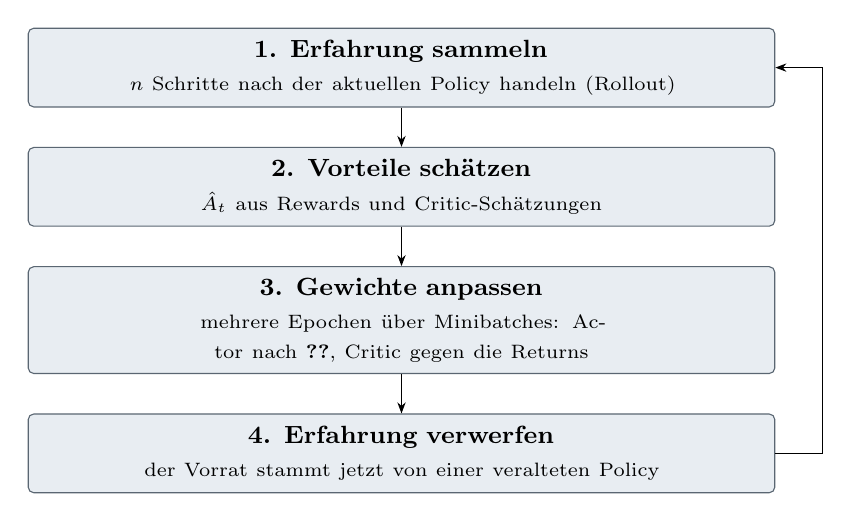
\begin{tikzpicture}[
    node distance=5mm,
    schritt/.style={draw=topoLine, line width=0.4pt, fill=topoNode,
      rounded corners=2pt, align=center, inner sep=4pt,
      text width=92mm, minimum height=10mm, font=\small},
    ->, >={Stealth[length=4pt]},
  ]
    \node[schritt] (a) {\textbf{1. Erfahrung sammeln}\\[1pt]
      {\scriptsize $n$ Schritte nach der aktuellen Policy handeln (Rollout)}};
    \node[schritt, below=of a] (b) {\textbf{2. Vorteile schätzen}\\[1pt]
      {\scriptsize $\hat{A}_t$ aus Rewards und Critic-Schätzungen}};
    \node[schritt, below=of b] (c) {\textbf{3. Gewichte anpassen}\\[1pt]
      {\scriptsize mehrere Epochen über Minibatches: Actor nach
      \Cref{eq:gradientenschritt}, Critic gegen die Returns}};
    \node[schritt, below=of c] (d) {\textbf{4. Erfahrung verwerfen}\\[1pt]
      {\scriptsize der Vorrat stammt jetzt von einer veralteten Policy}};
    % Ruecklaufkante rechts an allen Kaesten vorbei: Die Spalte (rand) liegt
    % ausserhalb der breitesten Box, damit der Pfeil keinen Kasten kreuzt.
    \coordinate (rand) at ([xshift=6mm]a.east);
    \draw (a) -- (b);
    \draw (b) -- (c);
    \draw (c) -- (d);
    \draw (d.east) -- (d.east -| rand) -- (a.east -| rand) -- (a.east);
  \end{tikzpicture}
  \caption[Trainingsschleife eines Actor-Critic-Verfahrens]{Trainingsschleife
  eines Actor-Critic-Verfahrens. Gehandelt wird in Schritt~1, gelernt erst in
  Schritt~3; zwischen zwei Lernphasen bleibt die Policy unverändert.}
  \label{fig:rl-schleife}
\end{figure}

Zwei Eigenschaften dieses Ablaufs sind später von Bedeutung. Erstens ist die
Policy zwischen zwei Lernphasen konstant, der Agent lernt also nicht nach jedem
einzelnen Schritt. Zweitens wird derselbe Vorrat mehrfach verwendet, was die
Zahl der benötigten Umgebungsschritte senkt, zugleich aber die Frage aufwirft,
wie weit sich die Policy dabei von derjenigen entfernen darf, mit der der Vorrat
gesammelt wurde. Genau daran setzt das im folgenden Abschnitt beschriebene
Verfahren an.

\subsection{Proximal Policy Optimization}
\label{sec:ppo}

\ac{A2C} und \ac{PPO} sind zwei verbreitete Verfahren, die beide der
Actor-Critic-Architektur folgen und regelmäßig miteinander verglichen
werden~\cite{delafuente2024comparative}. Sie unterscheiden sich darin, wie stark
ein einzelner Lernschritt die Policy verändern darf.

A2C sammelt wenige Schritte Erfahrung und aktualisiert die Policy daraufhin
unmittelbar~\cite[Abschn.~13.5]{suttonbarto2018}; die Schrittweite ist dabei
nicht nach oben begrenzt. Fällt ein Vorteil einmal ungewöhnlich groß aus, kann
eine einzelne Aktualisierung die Policy weit verschieben. Eine Aktion, die
zufällig einmal sehr gut ausging, wird dann sofort zur Gewohnheit, auch wenn sie
es nicht verdient hat. Schulman et al. benennen genau das als Schwäche des
unbeschränkten Vorgehens, das zu \glqq destructively large policy
updates\grqq{} führen könne~\cite[Abschn.~2.1]{schulman2017ppo}. \ac{PPO} setzt
dort an und deckelt die Verschiebung.

Gemessen wird sie an einer einzigen Größe: Um welchen Faktor ändert sich die
Wahrscheinlichkeit der Aktion, die tatsächlich gespielt wurde? Hielt die alte
Policy sie mit 20 Prozent für richtig und die neue mit 24 Prozent, so beträgt
dieser Faktor $24/20 = 1{,}2$. Formal ist das~\cite[Abschn.~3]{schulman2017ppo}
%
\begin{equation}
  \label{eq:ppo-ratio}
  r_t(\theta) = \frac{\pi_{\theta}(a_t \mid s_t)}{\pi_{\theta_{\text{alt}}}(a_t \mid s_t)}.
\end{equation}
%
Dabei steht $\theta$ für die Gewichte des Actor-Netzes, also für das, was beim
Training verändert wird, und $\theta_{\text{alt}}$ für ihren Stand vor der
Aktualisierung. Im Zähler steht die neue Wahrscheinlichkeit der Aktion $a_t$ im
Zustand $s_t$, im Nenner die alte. Ein Wert von eins bedeutet keine Änderung,
ein größerer Wert eine Erhöhung, ein kleinerer eine Verringerung.

Zu beachten ist, dass $r_t(\theta)$ keine einzelne Zahl je Lernschritt ist. Der
Index $t$ steht für einen bestimmten Zeitschritt, und das Verhältnis wird für
jedes im Rollout beobachtete Paar $(s_t, a_t)$ gesondert gebildet. Erst die
Mittelung über all diese Paare ergibt die Größe, die das Training maximiert.

Um diesen Faktor legt \ac{PPO} ein festes Band. Erlaubt ist nur der Bereich
zwischen $1-\varepsilon$ und $1+\varepsilon$, bei dem von Schulman et al.
vorgeschlagenen Wert $\varepsilon = 0{,}2$ also zwischen 0,8 und 1,2, was einer
Änderung von höchstens zwanzig Prozent
entspricht~\cite[Abschn.~3]{schulman2017ppo}. Verlässt der Faktor dieses Band,
wird er für die Berechnung auf den Randwert zurückgesetzt. Genau das leistet die
Funktion $\operatorname{clip}$ in der
Zielfunktion~\cite[Gl.~(7)]{schulman2017ppo}
%
\begin{equation}
  \label{eq:ppo-clip}
  L^{\text{CLIP}}(\theta) = \hat{\mathbb{E}}_t\!\left[
    \min\!\left(
      r_t(\theta)\,\hat{A}_t,\;
      \operatorname{clip}\!\left(r_t(\theta),\, 1-\varepsilon,\, 1+\varepsilon\right)\hat{A}_t
    \right)\right],
\end{equation}
%
die anstelle der Grundform aus \Cref{eq:policygradient} in
\Cref{eq:gradientenschritt} eingesetzt wird. Sie enthält drei Bestandteile. Der
geschätzte Vorteil $\hat{A}_t$ gibt an, ob die Aktion besser oder schlechter
ausfiel als erwartet. Der Faktor $r_t(\theta)$ davor sorgt dafür, dass eine
Erhöhung der Wahrscheinlichkeit bei positivem Vorteil den Ausdruck wachsen
lässt: Gute Aktionen wahrscheinlicher zu machen, lohnt sich. Das
$\hat{\mathbb{E}}_t$ ist der bereits eingeführte geschätzte Erwartungswert, hier
also der Mittelwert über alle Paare aus Zustand und Aktion des Rollouts.

Der Nutzen der Deckelung zeigt sich am Zahlenbeispiel. Eine Aktion sei mit
$\hat{A}_t = 5$ deutlich besser ausgefallen als erwartet, und die Aktualisierung
wolle ihre Wahrscheinlichkeit von 20 auf 40 Prozent anheben, also
$r_t(\theta) = 2$. Der linke Term im Minimum ergäbe dann $2 \cdot 5 = 10$, der
rechte dagegen nur $1{,}2 \cdot 5 = 6$, weil der Faktor dort auf 1,2 gestutzt
wird. Das Minimum wählt den kleineren Wert, hier also 6. Das ist genau der Wert,
den auch eine Anhebung auf lediglich 24 Prozent erbracht hätte. Über das Band
hinaus ist somit nichts mehr zu gewinnen, und der Anreiz zum großen Sprung
entfällt. Bei negativem Vorteil greift die Begrenzung spiegelbildlich auf der
Gegenseite und verhindert, dass die Wahrscheinlichkeit einer Aktion in einem Zug
fast auf null gedrückt wird.

Damit ist zugleich die am Ende von \Cref{sec:policyupdate} offene Frage
beantwortet: Der Vorrat darf mehrfach verwendet werden, weil die Deckelung
verhindert, dass sich die Policy dabei zu weit von derjenigen entfernt, mit der
er gesammelt wurde.

\subsection{Typische Schwierigkeiten}
\label{sec:rl-schwierigkeiten}

Fünf Eigenschaften des Ansatzes erschweren seinen Einsatz und werden im weiteren
Verlauf der Arbeit wiederholt eine Rolle spielen.

\paragraph{Hoher Bedarf an Erfahrung.}
Aus dem Credit-Assignment-Problem aus \Cref{sec:credit} folgt unmittelbar, dass
ein Agent sehr viele Schritte benötigt, bevor sich eine Bewertung festigt. Wo
überwachte Verfahren aus einem einzelnen eingestuften Beispiel unmittelbar
lernen, muss ein \ac{RL}-Agent denselben Zusammenhang über viele Episoden hinweg
wiederholt beobachten. Ein Training in der Realität scheidet dadurch für viele
Aufgaben aus.

\paragraph{Der Reward bestimmt das Verhalten vollständig.}
Ein Agent maximiert die Zielgröße, die ihm vorgegeben wird, und nicht die
Absicht dahinter. Belohnt eine Reward-Funktion versehentlich einen Vorgang, der
sich beliebig wiederholen lässt, ohne dass sich an der Lage etwas ändert, so
lernt der Agent genau diese Wiederholung. Sein Verhalten ist dann formal korrekt
und inhaltlich wertlos.

Damit ist die Reward-Hypothese aus \Cref{sec:rl-grundprinzip} nicht widerlegt,
aber ihre praktische Grenze benannt: Sie behauptet, dass sich ein Ziel als
skalare Größe ausdrücken \emph{lässt}, nicht, dass eine beliebige solche Größe
das gemeinte Ziel auch trifft. Ob beides zusammenfällt, entscheidet der Entwurf
der Reward-Funktion. Er ist deshalb kein Nebenaspekt, sondern bestimmt, was
überhaupt gemessen wird.

\paragraph{Mehrere lernende Agenten verletzen die Modellannahme.}
Der \ac{MDP} aus \Cref{sec:mdp} setzt eine konstante Übergangsfunktion voraus.
Handeln zwei Agenten im selben System und lernen beide gleichzeitig, so ist das
nicht mehr gegeben: Aus Sicht des einen verändert sich die Umgebung schon
dadurch, dass der andere seine Policy anpasst. Formal liegt dann kein \ac{MDP}
mehr vor, sondern ein \emph{Markov-Spiel}, und die Zielgröße verschiebt sich
fortlaufend. Aufgaben dieser Art sind Gegenstand des \ac{MARL}, das hier nicht
weiter verfolgt wird: Der Aufbau dieser Arbeit vermeidet die Schwierigkeit,
indem zu jedem Zeitpunkt nur einer der beiden Agenten lernt
(\Cref{sec:phasen}).

\paragraph{Unvollständige Beobachtbarkeit.}
Die Markov-Annahme verlangt, dass der beobachtete Zustand alle für die Zukunft
wesentliche Information enthält. In sicherheitsnahen Anwendungen ist das selten
erfüllt: Ein Angreifer kennt nur die Teile des Netzes, die er bereits entdeckt
hat. Ein Verteidiger sieht umgekehrt zwar den Zustand der eigenen Systeme und
damit auch, welche davon kompromittiert sind, nicht aber den Wissensstand des
Angreifers, also welche Knoten dieser bereits entdeckt und welche Zugangsdaten
er erbeutet hat. Beide beobachten den Zustand somit nur teilweise; formal liegt
dann ein \emph{teilweise beobachtbarer} Entscheidungsprozess vor.

In der Praxis wird die Abweichung überwiegend hingenommen und weiterhin ein
\ac{MDP} unterstellt. Gangupantulu et al. benennen den Grund: Die teilweise
beobachtbare Modellierung sei zwar realistischer, habe sich aber für große
Netze nicht als skalierbar erwiesen und verlange, zahlreiche
Wahrscheinlichkeitsverteilungen vorab zu
modellieren~\cite[Abschn.~II.C]{gangupantulu2021cja}. Die Verfahren werden also
angewendet, ohne dass ihre Voraussetzungen streng erfüllt sind, und das ist
eine bewusste Abwägung zwischen Wirklichkeitstreue und Handhabbarkeit.

\paragraph{Stochastik der Ergebnisse.}
Schließlich verläuft das Training selbst nicht deterministisch. Die
Initialisierung der Netze, die Ziehung der Aktionen aus der Policy und die
Umgebung selbst enthalten Zufall. Zwei Läufe desselben Aufbaus können deshalb
unterschiedlich ausfallen, weshalb ein einzelner Lauf eine Stichprobe darstellt
und kein Ergebnis.

\section{Grundbegriffe der Netzwerksicherheit}
\label{sec:netzsicherheit}

Dieser Abschnitt wechselt vom Lernverfahren zum Gegenstand. Er beschreibt
die Rollen von Angreifer und Verteidiger sowie den Ablauf eines Angriffs,
legt fest, was in dieser Arbeit unter einer Topologie verstanden wird, und
stellt die Segmentierungsmuster vor, aus denen die verglichenen Topologien
hervorgehen.

\subsection{Angreifer, Verteidiger und der Ablauf eines Angriffs}
\label{sec:angreifer-verteidiger}

Ein Netz besteht in der hier verwendeten Abstraktion aus \emph{Knoten}. Ein
Knoten steht für einen einzelnen Rechner, also einen \emph{Host}, der
\emph{Dienste} anbietet. Jeder Dienst lauscht auf einem \emph{Port} und verlangt
zur Anmeldung \emph{Zugangsdaten}. Welche Verbindungen zwischen zwei Knoten
überhaupt zustande kommen dürfen, regeln \emph{Firewall-Regeln}: Eine Freigabe
erlaubt Verkehr auf einem bestimmten Port, eine Sperre unterbindet ihn.

Der \emph{Angreifer} verfolgt das Ziel, Kontrolle über möglichst wertvolle
Systeme zu erlangen. Für diese wertvollsten Systeme hat sich der Begriff
\emph{Crown Jewels} eingebürgert. Gemeint sind diejenigen IT-Systeme, auf deren
bestimmungsgemäßen Betrieb eine Organisation angewiesen ist; wie kritisch ein
System ist, bemisst sich dabei an der Funktion, die es erfüllt, und an den
Daten, die es vorhält~\cite[Abschn.~II.A]{gangupantulu2021cja}.

Entscheidend an dieser Definition ist, dass sie nicht an der Netzstruktur
ansetzt, sondern an der Aufgabe der Organisation. Ermittelt werden Crown Jewels
in einem eigenen Verfahren, der \emph{Crown Jewels Analysis}, die die
Geschäftsaufgabe mit den vorhandenen IT-Werten abgleicht und jedem System einen
Relevanzwert zuweist; erst dadurch treten die betreffenden Systeme als die
wichtigsten und wertvollsten hervor~\cite[Abschn.~II.A]{gangupantulu2021cja}.
Derselbe Rechner kann somit in einer Organisation ein Crown Jewel sein und in
einer anderen ohne besondere Bedeutung.

Welches System diese Rolle in einem Netz einnimmt, ist damit keine Frage der
Technik, sondern eine Festlegung, die vorab getroffen werden muss.

Üblicherweise wird nicht der Weg in das Netz hinein modelliert, sondern der Weg
darin. Das \emph{Assumed-Breach-Prinzip} setzt voraus, dass ein erster Host
bereits kompromittiert ist, und fragt, was der Angreifer von dort aus erreicht.
Die Annahme ist realistisch, weil sich der erste Zugang, etwa über eine
Phishing-Nachricht, kaum zuverlässig verhindern lässt, und sie verschiebt den
Blick auf das, was danach geschieht.

Dieses Weiterarbeiten von einem übernommenen Host zum nächsten heißt
\emph{laterale Bewegung} und ist als eigene Taktik
definiert~\cite{mitreattack}. Sie setzt zweierlei voraus: einen Netzpfad zum
Ziel, den die Firewall zulassen muss, und gültige Zugangsdaten für das dort
laufende System. Beide Voraussetzungen sind voneinander unabhängig und müssen
gemeinsam erfüllt sein. Ein Angreifer, der ein Passwort
kennt, den betreffenden Rechner aber nicht erreicht, kommt nicht weiter.
Umgekehrt gilt dasselbe.

Ein Host, der einem Angreifer als Zwischenstation für solche Schritte dient,
heißt \emph{Pivot Point}, ein Knoten, den jeder Weg zu einem Ziel passieren
muss, \emph{Chokepoint}~\cite[Abschn.~II.A]{gangupantulu2021cja}. Ein Pivot
Point ist nicht zwingend selbst wertvoll; wird sein Risiko allein an seiner
eigenen Funktion bemessen, bleibt der Weg, den er eröffnet, unentdeckt.

Eine besondere Rolle nimmt dabei der \emph{Domain-Controller} ein, also der
Verzeichnisdienst, an dem sich die Systeme einer Windows-Domäne anmelden. Seine
Domänendatenbank enthält die Passwort-Hashes sämtlicher Domänenkonten, und deren
Auslesen ist als eigene Angriffstechnik dokumentiert~\cite{mitreattack_ntds}.
Ein Hash ist dabei noch kein Passwort: Er lässt sich offline durch
systematisches Ausprobieren einem Passwort zuordnen oder, je nach
Anmeldeverfahren, unmittelbar an dessen Stelle vorlegen. Wer den
Domain-Controller übernimmt, verfügt damit über die Anmeldeinformationen des
gesamten Netzes.

Der \emph{Verteidiger} verfolgt das Gegenziel und verfügt dafür über Maßnahmen,
die sich in zwei Gruppen einteilen lassen. \emph{Wiederherstellende} Maßnahmen
machen eine bereits eingetretene Kompromittierung rückgängig; das
\emph{Neuaufsetzen} eines Hosts, auch \emph{Reimaging} genannt, entzieht dem
Angreifer den Zugang zu diesem System. \emph{Präventive} Maßnahmen verhindern
einen Zugriff, bevor er stattfindet, etwa indem der eingehende Verkehr zu einem
gefährdeten System gesperrt wird.

Weder wiederherstellende noch präventive Maßnahmen sind kostenlos, und darin
liegt der eigentliche Zielkonflikt der Verteidigung. Ein neu aufgesetzter Host steht während des Vorgangs nicht zur
Verfügung, ein gesperrter Dienst ist auch für berechtigte Nutzer nicht mehr
erreichbar. Wie viel Ausfall hinnehmbar ist, wird als \emph{Verfügbarkeit}
gemessen und üblicherweise in einem \ac{SLA} festgeschrieben. Ein Verteidiger,
der das Netz vollständig abschaltet, hat zwar jeden Angriff unterbunden, aber
seine Aufgabe verfehlt.

\subsection{Netzwerktopologie als Sicherheitsarchitektur}
\label{sec:topologien}

Der Begriff Topologie wird uneinheitlich verwendet und bedarf daher einer
Festlegung. In dieser Arbeit bezeichnet er die Sicherheitsarchitektur eines
Netzes, also den Verlauf der Vertrauensgrenzen und die Frage, welche Systeme
miteinander kommunizieren dürfen. Gemeint ist ausdrücklich nicht die physische
Verkabelung: Graphentheoretische Muster wie Bus, Ring oder Stern beschreiben die
Verdrahtung von Geräten und liegen auf einer anderen Abstraktionsebene.

Der Grund für diese Festlegung liegt darin, dass die Verkabelung nichts darüber
aussagt, wer worauf zugreifen darf. Zwei Systeme am selben Switch können durch
Zugriffsregeln vollständig voneinander getrennt sein, während zwei Systeme an
entgegengesetzten Enden eines Gebäudes uneingeschränkt miteinander
kommunizieren. Für einen Angreifer, der sich lateral bewegt, ist allein
maßgeblich, welche Zugriffe zugelassen sind.

Die Zero-Trust-Architektur des \ac{NIST} verlagert den Maßstab in dieselbe
Richtung, von der Lage eines Systems auf die für es geltenden Regeln.
Ihr zweiter Grundsatz lautet, dass die Position im Netz für sich genommen kein
Vertrauen begründet; die zugehörigen Annahmen halten fest, dass das gesamte
private Unternehmensnetz nicht als implizite Vertrauenszone gelten
darf~\cite[Abschn.~2.1--2.2]{nist800207}. Über einen Zugriff entscheidet danach
nicht die Zugehörigkeit zu einem Netzabschnitt, sondern eine ausdrückliche
Regel. Damit ist die Ebene benannt, auf der diese Arbeit den Topologiebegriff
ansiedelt: die der zugelassenen Kommunikationsbeziehungen.

Das Mittel dazu ist die \emph{Segmentierung}. Sie unterbindet nicht benötigte
Kommunikationspfade und erschwert damit genau die laterale Bewegung aus
\Cref{sec:angreifer-verteidiger}: Ein Angreifer, der einen Host übernommen hat,
erreicht von dort aus weniger Systeme, als er es in einem unsegmentierten Netz
täte. Genau darin unterscheiden sich die im folgenden Abschnitt beschriebenen
Muster.

\subsection{Segmentierungsmuster}
\label{sec:segmentierungsmuster}

Die gebräuchlichen Muster lassen sich als Spektrum auffassen, das vom
unsegmentierten Netz bis zur feingranularen Trennung einzelner Systeme reicht.
Vier davon werden in dieser Arbeit verglichen; ihre konkrete Umsetzung
beschreibt \Cref{sec:topomodell}.

\paragraph{Flach.}
Ein flaches Netz kennt keine interne Segmentierung. Alle Hosts liegen in
derselben Vertrauenszone, jeder erreicht jeden. Das ist der Ausgangszustand, den
die Zero-Trust-Literatur als Risiko benennt: Ein einziger kompromittierter Host
genügt, um sich frei im gesamten Netz zu bewegen~\cite{nist800207}.

\paragraph{DMZ.}
Die \ac{DMZ} führt eine grobe Zonentrennung ein. Von außen erreichbare Dienste
stehen in einer entmilitarisierten Zone, die per Firewall vom internen Netz
getrennt ist~\cite{nist800041}. Der Perimeter ist damit befestigt, das Innere
bleibt aber vergleichsweise offen. Für einen Angreifer bedeutet das eine Hürde
beim Übertritt in das Intranet, danach jedoch vergleichsweise freie Bewegung.

\paragraph{Hub-and-Spoke.}
Das Hub-and-Spoke-Modell fällt aus der Reihe, weil es nicht mit Zonen arbeitet,
sondern sämtliche Zugriffe über einen einzigen Knoten führt. Als
Referenzarchitektur ist es dadurch gekennzeichnet, dass die Verbindungen nicht
transitiv sind: Jeder Spoke ist mit dem Hub verbunden, kein Spoke mit einem
anderen. Die Arbeitslasten der Spokes sind damit voneinander getrennt, während
die zentrale Zugriffskontrolle im Hub liegt~\cite{mshubspoke}. Der Hub ist
damit ein Chokepoint im Sinne von \Cref{sec:angreifer-verteidiger}, und zwar
ein baulich erzwungener: Er entsteht nicht dadurch, dass ein Angreifer diesen
Weg wählt, sondern dadurch, dass kein anderer existiert.

Der Begriff selbst stammt aus der Praxis der Netzarchitektur und ist in keinem
Standard normiert, das zugrunde liegende Prinzip ist es sehr wohl: \ac{NIST}
verlangt für eine Zero-Trust-Architektur, dass Ressourcen ohne Passieren eines
Kontrollpunkts nicht erreichbar sind~\cite[Abschn.~3.4.1]{nist800207}.
Hub-and-Spoke ist die bauliche Umsetzung dieses Gedankens: ein einziger Punkt,
an dem jeder Weg vorbeiführt.

Der Preis des Musters ist eine ausgeprägte Abhängigkeit, denn die Trennung der
Spokes ruht vollständig auf diesem einen Punkt. Geht die Kontrolle über ihn
verloren, entfällt sie ersatzlos. Realisiert wird der Hub deshalb üblicherweise
nicht durch ein Endsystem, sondern durch ein eigens dafür vorgesehenes und
entsprechend gehärtetes Gerät.

\paragraph{Micro-Segmentierung.}
Micro-Segmentierung treibt die Trennung auf die Ebene einzelner Systeme. Erlaubt
ist nur, was explizit nötig ist, und jede Verbindung wird verifiziert. Das
entspricht dem Zero-Trust-Prinzip~\cite{nist800207}. Über die Erreichbarkeit
hinaus betrifft der Grundsatz auch die Zugangsdaten: Zugriffe sollen je Sitzung
geprüft werden, statt dauerhaft gültige Berechtigungen auf den Systemen
vorzuhalten~\cite[Abschn.~2.1]{nist800207}. Beides zusammen verkürzt die Wege
eines Angreifers nicht, sondern verlängert sie, weil er für jeden Schritt sowohl
einen zugelassenen Pfad als auch die passenden Zugangsdaten benötigt.

\section{Stand der Forschung}
\label{sec:sota}

Dieser Abschnitt ordnet die Arbeit in die vorhandene Literatur ein. Er
stellt die verfügbaren Simulationsumgebungen für Netzwerkangriffe vor,
prüft, inwieweit sie einen lernenden Verteidiger vorsehen, und beschreibt
mit MARLon die Erweiterung, auf der der eigene Aufbau beruht.

\subsection{Simulationsumgebungen für Netzwerkangriffe}
\label{sec:umgebungen}

Ein \ac{RL}-Agent lernt aus Erfahrung und benötigt dafür nach
\Cref{sec:rl-schwierigkeiten} sehr viele Episoden. In einem produktiven
Firmennetz ist das weder praktikabel noch verantwortbar. Das Training findet
deshalb in einer eigens gebauten Umgebung statt, die die für laterale Bewegung
wesentlichen Mechanismen nachbildet, ohne ein reales Netz in allen Details zu
kopieren. Einen Überblick über \ac{RL}-Verfahren in der Cybersicherheit
insgesamt geben Nguyen und Reddi~\cite{nguyen2023drl}.

Solche Umgebungen unterscheiden sich vor allem entlang einer Achse. Eine
\emph{Simulation} bildet das Netz als abstraktes Modell im Programm nach; ein
Schritt kostet dann nur die Rechenzeit für eine Zustandsänderung. Eine
\emph{Emulation} betreibt stattdessen echte Systeme, etwa virtuelle Maschinen
mit realer Netzanbindung, sodass ein Schritt tatsächlich ausgeführt wird. Die
Emulation ist wirklichkeitsnäher, die Simulation um Größenordnungen schneller.

\paragraph{CyberBattleSim.}
\ac{CBS}~\cite{cyberbattlesim2021} ist eine Simulation von Microsoft. Sie bildet
ein Netzwerk als gerichteten Graphen ab; jeder Knoten steht für einen Host mit
Diensten, Schwachstellen und einer Firewall-Konfiguration. Der Angreifer beginnt
nach dem Assumed-Breach-Prinzip auf einem bereits kompromittierten
Einstiegsknoten. Eine Aktion ist etwa das Ausnutzen einer lokalen oder
entfernten Schwachstelle oder der Verbindungsaufbau zu einem weiteren Knoten mit
zuvor erbeuteten Zugangsdaten. Das Netz wird unmittelbar im Programmcode als
Graph definiert, sodass sich Knoten, Zugangsdaten und Firewall-Regeln gezielt
setzen lassen. Bereitgestellt wird die Umgebung über die
\emph{Gym-Schnittstelle}~\cite{cyberbattlesim2021}, die festlegt, wie eine
Umgebung ihren Zustand zurückgibt und eine Aktion entgegennimmt. Auf derselben
Schnittstelle setzt auch \ac{SB3} auf~\cite{stablebaselines3}, sodass sich beide
ohne Anpassung verbinden lassen.

\paragraph{CybORG.}
CybORG~\cite{standen2021cyborg} verfolgt einen zweigleisigen Ansatz und stellt
sowohl einen Simulations- als auch einen Emulationsmodus bereit, wobei letzterer
über eine Cloud-Infrastruktur betrieben wird. Das dokumentierte Szenario umfasst
drei Hosts in zwei Subnetzen. Die Umgebung ist zugleich der Ausgangspunkt der
CAGE-Wettbewerbe und damit vor allem auf vergleichbare, vorgegebene
Aufgabenstellungen ausgelegt.

\paragraph{CyGIL.}
CyGIL~\cite{li2021cygil} ist eine Emulation, die Aktionen auf tatsächlich
betriebenen virtuellen Maschinen ausführt. Die dokumentierten Szenarien umfassen
vier beziehungsweise neun Hosts. Der Preis der Wirklichkeitstreue ist die
Laufzeit: Nach eigener Messung dauert eine Episode etwa 30 Sekunden im kleineren
und 20 bis 30 Minuten im größeren Szenario, das Training eines einzelnen Agenten
entsprechend Stunden bis Tage. Eine spätere Ausbaustufe ergänzt mit CyGIL-S
einen Simulator, der aus Daten des Emulators erzeugt wird und dessen Betrieb
damit voraussetzt~\cite{li2023cygilsim}.

\paragraph{Angriffsgraphen als Gegenentwurf.}
Ein zweiter Zweig der Literatur verzichtet ganz auf eine ausführbare
Nachbildung des Netzes und fasst stattdessen einen vorab erzeugten
\emph{Angriffsgraphen} unmittelbar als \ac{MDP} auf, dessen
Übergangswahrscheinlichkeiten aus Bewertungskennzahlen bekannter Schwachstellen
stammen~\cite[Abschn.~II.C]{gangupantulu2021cja}. Der Ansatz skaliert auf
Graphen mit mehreren tausend Knoten, setzt aber voraus, dass sich der Verlauf
eines Angriffs vorab vollständig niederschreiben lässt, und kennt keinen
zweiten, gleichzeitig handelnden Agenten.

Welche dieser Umgebungen für die vorliegende Arbeit gewählt wurde und aus
welchen Gründen, behandelt \Cref{sec:umgebungswahl}.

\subsection{Lernende Agenten auf beiden Seiten}
\label{sec:beidseitig}

Ein Merkmal zieht sich durch die genannten Arbeiten: Trainiert wird
üblicherweise der Angreifer. Der Verteidiger ist, sofern überhaupt vorhanden,
eine feste regelbasierte Komponente.

CybORG erprobt in seiner Ursprungsfassung einen einzigen angreifenden Agenten
und führt die für einen lernenden Verteidiger nötigen Aktionen, Sensoren und
Aktuatoren als ersten Punkt der künftigen Arbeiten
auf~\cite{standen2021cyborg}. CyGIL ist ausdrücklich nur für das Training von
Angreifern erprobt~\cite{li2021cygil}; auch die spätere Ausbaustufe sieht zwar
begrifflich einen verteidigenden Agenten vor, trainiert in sämtlichen
Experimenten aber weiterhin allein den angreifenden~\cite{li2023cygilsim}. Dieselbe Einschränkung gilt für \ac{CBS}
selbst, wie die Autoren von CybORG in ihrem Vergleich feststellen: Ein fester
Verteidiger sei möglich, dessen Training jedoch nicht
vorgesehen~\cite{standen2021cyborg}.

Für eine Frage nach der \emph{Lerneffizienz eines Verteidigers} ist das die
entscheidende Lücke, denn sie lässt sich ohne einen zweiten lernenden Agenten
nicht stellen. Zugleich führt ein solcher Aufbau in die in
\Cref{sec:rl-schwierigkeiten} genannte Schwierigkeit: Lernen beide Seiten
gleichzeitig, liegt kein \ac{MDP} mehr vor.

\subsection{MARLon}
\label{sec:cbs}

MARLon~\cite{marlon} schließt genau diese Lücke für \ac{CBS}. Es erweitert
die Umgebung um einen zweiten, ebenfalls lernenden Agenten für die Verteidigung;
beide handeln abwechselnd im selben Netz. Bereitgestellt werden dafür
Implementierungen von \ac{A2C} und \ac{PPO} aus der Bibliothek
\ac{SB3}~\cite{stablebaselines3}, jeweils für Angreifer wie Verteidiger.

Der Verteidiger erhält dabei eine an den Angreifer gekoppelte Bewertung, und
sein Aktionsraum umfasst Maßnahmen wie das Neuaufsetzen eines Knotens sowie das
Sperren und Freigeben von Verkehr. Die genaue Ausgestaltung dieser Kopplung, die
sich für die vorliegende Arbeit als folgenreich erwiesen hat, behandelt
\Cref{sec:marlon-original}.

MARLon ist damit die Grundlage der vorliegenden Arbeit. Welche Anpassungen daran
nötig waren, beschreibt \Cref{ch:versuchsaufbau}.

\chapter{Versuchsaufbau}
\label{ch:versuchsaufbau}

Untersucht wird, ob und wie stark die Netzwerktopologie beeinflusst und wie
schnell und wie gut ein Verteidigungsagent lernt. Die Topologie ist die
unabhängige Variable, jedoch nicht der einzige variierte Faktor: Der
Verteidiger trainiert stets gegen einen bestimmten eingefrorenen Angreifer.
Ob und in welchem Umfang dessen Herkunft die Aufgabe beeinflusst, ist offen und
selbst Teil der Untersuchung. Beide Größen werden deshalb systematisch
gekreuzt, sodass sich ihre Beiträge trennen lassen (\Cref{sec:phasen}).

Alles Übrige muss konstant gehalten werden, sonst lassen sich beobachtete
Unterschiede nicht mehr zuordnen. Bevor dieser Aufbau im Einzelnen beschrieben
wird, ist jedoch ein Umweg nötig: Der hier verwendete Reward und Aktionsraum
sind nicht die von MARLon übernommenen, sondern eine eigene Überarbeitung.
\Cref{sec:vorarbeiten} begründet, warum diese Überarbeitung nötig wurde.

\section{Von MARLon zum eigenen Aufbau}
\label{sec:vorarbeiten}

Dieser Abschnitt beschreibt, wie aus dem übernommenen Rahmenwerk der in
dieser Arbeit verwendete Aufbau wurde. Er benennt zunächst den geerbten
Ausgangspunkt, schildert dann einen vollständigen Durchgang durch die
Versuchsmatrix und die drei Fehler, die dieser sichtbar machte, und begründet
daraus die anschließende Überarbeitung.

\subsection{Der geerbte Ausgangspunkt}
\label{sec:marlon-original}

MARLon~\autocite{marlon} stellt die Trainingsumgebung für beide Agenten
bereit, wie in \Cref{sec:cbs} beschrieben. Für den Verteidiger legt die
Originalarbeit dabei eine bestimmte Reward-Struktur fest: Sein Reward ergibt
sich durch Negation des jeweils letzten Angreifer-Rewards, ergänzt um eine
große Strafe bei Unterschreiten der Netzverfügbarkeit. Die Autoren begründen
diese Wahl damit, dass der Verteidiger den Fortschritt des Angreifers
minimieren solle, und halten als unmittelbare Folge fest, dass sein maximal
erreichbarer Reward damit bei null liegt und mit jedem Fortschritt des
Angreifers weiter sinkt~\autocite{marlon}. Prävention ist in dieser Formel nicht vorgesehen, und einen Anreiz zur
Rückeroberung enthält sie ebenso wenig: \ac{CBS} schreibt den Knotenwert nur bei der ersten Übernahme gut, sodass
ein späterer Besitzwechsel desselben Knotens den Reward beider Seiten
unverändert lässt. Gefördert wird damit gerade nicht das Verhalten, auf das
es in dieser Arbeit ankommt: den Angreifer am Vordringen zu hindern und
bereits verlorene Systeme zurückzugewinnen.

Für den Aktionsraum des Verteidigers sieht MARLon fünf Aktionsarten vor:
%
\begin{enumerate}
  \item einen Knoten neu aufsetzen,
  \item Verkehr sperren,
  \item Verkehr freigeben,
  \item einen Dienst stoppen,
  \item einen Dienst wieder starten.
\end{enumerate}
%
Port und Richtung sind dabei zusätzliche Parameter, die der Agent selbst
wählt. Für den Angreifer
identifiziert die Originalarbeit den Umgang mit ungültigen Aktionen als eigenes
Problem. Gültig ist eine Aktion, wenn der Angreifer sie im aktuellen Zustand
überhaupt versuchen kann: Der Ausgangsknoten muss übernommen, das Ziel entdeckt
und die eingesetzten Zugangsdaten müssen bereits erbeutet sein. Ob der Versuch
gelingt, entscheidet sich unabhängig davon. Ein Verbindungsversuch auf einen
Port, auf dem das Ziel keinen Dienst anbietet, ist eine gültige Aktion, die
lediglich folgenlos bleibt. Eine Bestrafung ungültiger Aktionen würde dazu
führen, dass der Agent riskante, aber
notwendige Aktionen ganz meidet; die Autoren entscheiden sich stattdessen für
Reward~0 bei ungültigen Aktionen, kombiniert mit einer zufälligen
Ersatzwahl. Diese Entscheidung ist im Code der Umgebung selbst verankert, nicht
nur im Trainingsablauf.

\subsection{Eigene Vorarbeiten und der Referenzlauf}
\label{sec:referenzlauf}

Dass der Verteidiger damit weder für verhinderte noch für rückgängig
gemachte Übernahmen etwas erhält, war der Anlass, seinen Reward in mehreren
Schritten zu überarbeiten. Ein zwischenzeitlicher
Entwurf war ereignisbasiert und vergütete jedes Neuaufsetzen eines
kompromittierten Knotens mit einem festen Betrag. Damit belohnte er einen
beliebig wiederholbaren Vorgang, und
zwar einseitig: \ac{CBS} schreibt einen Knotenwert nur bei der ersten Übernahme
gut, sodass dem Angreifer eine Rückeroberung nichts einbrachte, während der
Verteidiger für jedes Neuaufsetzen desselben Knotens erneut vergütet wurde. Ein
einzelner Knoten wechselte dadurch fortwährend zwischen kompromittiert und neu
aufgesetzt, ohne dass sich die Lage im Netz über einen solchen Zyklus hinweg
verändert hätte, und der Verteidiger wurde für jede Runde erneut belohnt. Das ist genau
der in \Cref{sec:rl-schwierigkeiten} beschriebene Fall, in dem ein Agent formal
korrekt maximiert und inhaltlich nichts erreicht. Daraufhin wurde zur Kopplung
aus \Cref{sec:marlon-original} zurückgekehrt, die MARLon ursprünglich vorsieht.

Über diese Kopplung hinaus umfasste der Aufbau zu diesem Zeitpunkt vier
eigene Ergänzungen:
%
\begin{enumerate}
  \item vier Vergleichstopologien anstelle des einen von MARLon
        vorgesehenen festen Netzes (\Cref{sec:topomodell}),
  \item ein Invalid-Action-Masking für den Angreifer nach Huang und
        Ontañón~\autocite{huang2022masking}, das MARLons
        Zufallsersatzverfahren ablöst (\Cref{sec:masking}),
  \item ein Haltebonus je gehaltenem Knoten und Zeitschritt
        (\Cref{sec:rewards}),
  \item ein Abzug in Höhe des Knotenwerts, wenn ein gehaltener Knoten neu
        aufgesetzt wird (\Cref{sec:rewards}).
\end{enumerate}
%
Die zweite Ergänzung verdient eine Erläuterung: Statt eine ungültige Aktion
zu raten und auf eine zufällige gültige auszuweichen, wählt der Angreifer
ausschließlich aus der im jeweiligen Zustand gültigen Menge. Wirkungslose
Aktionen entfielen dadurch praktisch vollständig, und der Angreifer
erreichte das Crown Jewel zuverlässig, statt wie zuvor nur in
Ausnahmefällen. Erst das machte ihn als Gegner brauchbar, denn die
Lerneffizienz eines Verteidigers lässt sich nur gegen einen Angreifer
messen, der überhaupt etwas ausrichtet.

Von der übernommenen Reward-Struktur blieben damit zwei Bestandteile unberührt,
und gerade sie bestimmen die erreichbare Obergrenze: die Kopplung des
Verteidiger-Rewards an den negierten Angreifer-Reward und die Begrenzung des
Angreifer-Schrittwerts nach unten auf null. Letztere ist in \ac{CBS} selbst
verankert und wurde bewusst beibehalten; \Cref{sec:rewards} legt dar, weshalb.
Die eigenen Ergänzungen verschieben den Angreifer-Reward, heben diese
Obergrenze aber nicht auf.

Auf diesem Stand entstand der im Folgenden als \emph{Referenzlauf} bezeichnete
Durchgang durch die vollständige Versuchsmatrix. Er ist der Vergleichsmaßstab
dieser Arbeit: Sein Ergebnis begründet die anschließend vorgenommenen
Änderungen am Aufbau, und an ihm wird deren Wirkung gemessen. Die Schwächen,
die die folgenden Abschnitte beschreiben, wurden erst durch ihn sichtbar und
waren zum Zeitpunkt seiner Durchführung nicht bekannt. Darin unterscheidet er
sich von den übrigen Zwischenständen des Aufbaus, die nur dort zur Sprache
kommen, wo sie eine Entwurfsentscheidung erklären. Die Matrix kreuzt die vier
Verteidigungstopologien mit sechs Angreifern: fünf davon wurden auf jeweils
genau einer Topologie trainiert, ein sechster nacheinander auf allen. Wegen der
in \Cref{sec:rl-schwierigkeiten} genannten Stochastik wird jede der
24~Kombinationen fünfmal wiederholt, jeweils mit einem anderen Startwert für die
Zufallsgeneratoren, einem sogenannten \emph{Seed}. Das ergibt
\num{120}~Trainingsläufe.

Als Budget waren dabei je \num{500000} Schritte vorgesehen, ausgeschöpft wurde
es aber nicht durchgängig: Das Konvergenzkriterium aus \Cref{sec:konvergenz}
diente im Referenzlauf noch als Abbruchbedingung und beendete das Training,
sobald es erfüllt war. Für die später berichteten Läufe wurde davon abgerückt;
\Cref{sec:konvergenz} begründet das. Die vier Ergänzungen sind
auch im überarbeiteten Aufbau enthalten und werden in den folgenden
Abschnitten beschrieben; was erst nach dem Referenzlauf hinzukam, ist
Gegenstand von \Cref{sec:konsequenz}.

Das Ergebnis bestätigte, was \Cref{sec:marlon-original} bereits aus der Formel
ableitet: In allen \num{8642} protokollierten Trainingsepisoden war der
Verteidiger-Reward negativ, der höchste beobachtete Einzelwert betrug
$-14{,}0$. Das ist keine Fehlfunktion, sondern die Obergrenze null, empirisch
bestätigt. Für eine Metrik, die ursprünglich vorgesehen war, hat das
unmittelbare Folgen: Break-even, definiert als die Episode, ab der der
geglättete Reward nicht mehr negativ ist, kann unter dieser Kopplung
strukturell nie eintreten und entfällt deshalb vollständig
(\Cref{sec:metriken}).

\subsection{Drei Fehler in der Umsetzung}
\label{sec:marlon-fehler}

Über die reine Reward-Formel hinaus fanden sich drei Stellen, an denen die
Sperre als Mittel der Prävention beeinträchtigt war. Sämtliche drei wurden erst
nach dem Referenzlauf behoben und waren während seiner gesamten Dauer wirksam.

Der erste betrifft die Liste der sperrbaren Ports und ist der eigenen Arbeit
zuzurechnen. MARLon hält sie fest verdrahtet im Code, passend zu der
Umgebung, für die das Rahmenwerk entworfen wurde; dort ist sie zutreffend. Mit
den in \Cref{sec:topomodell} beschriebenen Topologien kamen jedoch andere
Dienste ins Netz, und die Liste wurde dabei nicht mitgeführt. Von den sechs
tatsächlich vorkommenden Ports fehlten ihr zwei, während sie zwei weitere
enthielt, die in keiner der Topologien auftreten. Der Datenbank-, der Backup-
und der Dateiserver, darunter das Crown Jewel, ließen sich dadurch nie
ansprechen. Für die späteren Läufe wird die Liste nicht mehr fest vorgegeben,
sondern aus der Umgebung abgeleitet und folgt damit jeder Topologie.

Die beiden folgenden Punkte stammen dagegen aus dem unveränderten
MARLon-Code. Sie blieben im Referenzlauf ohne Folgen und wurden erst durch
die spätere Überarbeitung zum Hindernis; der Vollständigkeit halber gehören sie
dennoch hierher.

Die Methode zum Sperren von Verkehr entfernte lediglich eine vorhandene
Freigabe-Regel, statt eine ausdrückliche Sperr-Regel zu setzen. Unterbunden war
der Verkehr danach tatsächlich, weil \ac{CBS} einen Port ohne Regel als gesperrt
behandelt. Ein so gesperrter Port sah anschließend jedoch genauso aus wie einer,
für den nie eine Freigabe bestand, und das ist in den hier verwendeten
Topologien der bauliche Normalzustand: Sie arbeiten mit Freigabelisten, sodass
die meisten Ports ohnehin keine Regel tragen. Ein Eingriff des Verteidigers war
damit nicht mehr von der Ausgangslage zu unterscheiden. Für den Angreifer
änderte das nichts, denn er stieß in beiden Fällen auf eine geschlossene Tür.
Sobald jedoch der Reward eine bewusst gesetzte Sperre erkennen und belohnen
soll, wie in \Cref{sec:rewards} beschrieben, ist die Unterscheidung
unentbehrlich. Die zugehörige Methode zum Freigeben von Verkehr war zudem
fehlerhaft: Beide Zweige der Fallunterscheidung schrieben in die eingehende
Regelliste, sodass sich eine ausgehende Sperre nicht wieder aufheben ließ.

Schließlich zählte die Verfügbarkeitsberechnung nur, ob ein Dienst läuft, nicht
aber, ob sein Port gesperrt ist. Sperren kostete damit keine Verfügbarkeit. Im
Referenzlauf fiel auch das nicht ins Gewicht, weil eine Sperre dort ohnehin
nichts einbrachte. Wird sie dagegen belohnt, entsteht daraus ein Fehlanreiz:
Der Verteidiger könnte das Netz vollständig abriegeln, ohne dafür je das
\ac{SLA} zu verletzen.

Für den Referenzlauf bleibt damit vor allem der erste Punkt. Er allein erklärt
noch nicht, warum der Verteidiger ausschließlich das Neuaufsetzen lernte, denn
die entscheidende Ursache liegt in der Reward-Formel: Ein verhinderter Zugriff
bringt dem Angreifer null ein und dem Verteidiger über die Kopplung ebenfalls
null. Die fehlerhafte Portliste kam hinzu und schloss die wertvollsten Systeme
von vornherein aus. Und die einzige verbliebene präventive Handlung wurde sogar
bestraft: Das Stoppen eines Dienstes auf einem nicht kompromittierten Knoten
kostete zehn Punkte, und da sich nicht vorhersehen lässt, welchen Knoten der
Angreifer als Nächstes angreift, traf diese Strafe den Verteidiger regelmäßig.
Von den präventiven Mitteln blieb ihm keines, das sich gelohnt hätte.

\subsection{Konsequenz für diese Arbeit}
\label{sec:konsequenz}

Aus diesem Befund folgt nicht, dass sich mit der Fragestellung nach dem
Einfluss der Topologie nichts anfangen ließe. Der Referenzlauf bleibt
verwertbar, allerdings für eine engere Aussage, als ursprünglich
beabsichtigt: Er beschreibt einen Verteidiger, der ausschließlich reaktiv
handeln kann, also Wiederherstellung statt Prävention. Reimaging ist selbst
eine Form der Abwehr, denn es entzieht dem Angreifer den Zugang und macht
dessen Gewinn rückgängig, auch wenn es keinen Angriff verhindert.

Für die in dieser Arbeit berichteten Ergebnisse wurde der Aufbau aus zwei Gründen
grundlegend überarbeitet: Erstens lassen sich die drei in
\Cref{sec:marlon-fehler} genannten Punkte als Implementierungsfehler und nicht
als Entwurfsentscheidungen einordnen; sie zu beheben ist unabhängig von der
Forschungsfrage geboten. Zweitens lässt erst ein Verteidiger, der Prävention
tatsächlich ausführen und dafür belohnt werden kann, die Frage nach dem
Einfluss der Topologie auf einen \emph{präventiven} Verteidiger überhaupt
zu; unter dem Referenzlauf wäre jede Topologie mit derselben Unmöglichkeit
konfrontiert gewesen. Die folgenden Abschnitte beschreiben den überarbeiteten
Aufbau, wie er den in \Cref{ch:ergebnisse} berichteten Läufen zugrunde liegt.
Wo eine Änderung das Ergebnis unmittelbar beeinflusst, wird auf den Referenzlauf
als Vergleichspunkt zurückverwiesen.

\section{Wahl der Simulationsumgebung und des Lernverfahrens}
\label{sec:umgebungswahl}

Zwei Entscheidungen liegen dem Versuch zugrunde, bevor sich Fragen seiner
Ausgestaltung stellen: in welcher Simulationsumgebung er stattfindet und
mit welchem Lernverfahren die Agenten trainiert werden. Dieser Abschnitt
begründet beide.

\subsection{Die Simulationsumgebung}

Von den in \Cref{sec:umgebungen} vorgestellten Umgebungen fiel die Wahl auf \ac{CBS} in Verbindung mit MARLon. Maßgeblich dafür sind drei
Anforderungen, die sich unmittelbar aus der Fragestellung ergeben: eine frei
definierbare Netzwerktopologie, ein lernender Agent auf beiden Seiten und ein
Durchsatz, der eine Versuchsmatrix dieses Umfangs erlaubt. Die beiden
Alternativen scheitern jeweils an mehreren dieser Anforderungen.

Zu beachten ist dabei, dass alle drei Umgebungen fortlaufend weiterentwickelt
werden. Der folgende Vergleich bezieht sich auf den Stand, den die jeweiligen
Veröffentlichungen dokumentieren; spätere Erweiterungen sind, soweit sie belegt
sind, angeführt.

Die erste Anforderung ist die entscheidende, weil sie den Untersuchungsgegenstand
selbst betrifft. Dass \ac{CBS} das Netz unmittelbar im Programmcode als
Graph definiert (\Cref{sec:umgebungen}), ermöglicht erst den in
\Cref{sec:umgebung}
beschriebenen Aufbau, in dem sich die vier Topologien allein in ihrer
Segmentierung unterscheiden, während Knotenzahl und Knotenwerte konstant
bleiben. Die dokumentierten Szenarien der beiden anderen Umgebungen sind
demgegenüber klein und auf andere Zwecke zugeschnitten. Eine Topologie zu
verändern bedeutet dort, die zugrunde liegende Infrastruktur umzubauen.

Die zweite Anforderung betrifft die Gegenseite. Der Verteidiger soll sich gegen
ein Angriffsverhalten behaupten, das seinerseits aus Erfahrung entstanden ist
und nicht aus einer festen Regel. Wie \Cref{sec:beidseitig} zeigt, ist der
lernende Verteidiger in beiden Alternativen jedoch nicht umgesetzt. Genau diese
Lücke schließt MARLon, indem es für beide Rollen \ac{RL}-Agenten bereitstellt.

Die dritte Anforderung ist eine praktische. Die in dieser Arbeit ausgewerteten
120 Trainingsläufe umfassen zusammen rund 60~Millionen
Simulationsschritte.
Rechnet man die für CyGIL dokumentierten Episodendauern
(\Cref{sec:umgebungen}) auf diesen Umfang hoch, liegt das Ergebnis jenseits
des für eine Abschlussarbeit verfügbaren Zeitrahmens; der dort ebenfalls
genannte Simulator CyGIL-S nimmt diese Hürde nicht, weil er den Betrieb des
Emulators voraussetzt. CybORG bietet zwar
einen reinen Simulationsmodus, betreibt seinen Emulator jedoch über eine
Cloud-Infrastruktur~\cite{standen2021cyborg}, was neben dem Zeit- auch einen
Kostenaufwand nach sich zieht.

Mit der Wahl wird zugleich eine Einschränkung übernommen: Als reine Simulation
bildet \ac{CBS} keine echten Systeme ab, sodass die Übertragbarkeit der
Ergebnisse auf reale Netze offenbleibt. Die höhere Wirklichkeitstreue der
emulationsbasierten Ansätze wäre hier gegen die Zahl der durchführbaren Läufe
einzutauschen gewesen. Da die Fragestellung auf den \emph{Vergleich} von
Topologien unter sonst gleichen Bedingungen zielt und nicht auf absolute
Aussagen über konkrete Netze, wiegt die Zahl der Läufe schwerer.
\Cref{sec:limitationen} greift diesen Punkt erneut auf.

\subsection{Das Lernverfahren}

MARLon stellt mit \ac{A2C} und \ac{PPO} zwei Verfahren aus \ac{SB3} bereit
(\Cref{sec:cbs}). Für beide existieren vollständige, parallel gepflegte
Implementierungen für Angreifer wie Verteidiger, sodass die Wahl offensteht.
Sie fiel auf \ac{PPO}.

Die in \Cref{sec:ppo} beschriebene Deckelung erzeugt gleichmäßigere
Lernkurven, da einzelne Ausreißer den bisherigen Lernfortschritt nicht in einem
Schritt verwerfen können. Betroffen ist davon nicht allein die Darstellung,
sondern die Messbarkeit: Zu den erhobenen Größen gehört die Lerneffizienz und
damit der Zeitpunkt, zu dem ein Lauf als konvergiert gilt, und
das Konvergenzkriterium in \Cref{sec:konvergenz} entscheidet anhand der
Streuung und des Trends der Episoden-Rewards innerhalb eines Fensters. Ein
Verfahren, dessen Kurve wiederholt springt, würde dieses Kriterium unabhängig
von der Topologie später auslösen und die Vergleichbarkeit zwischen den
Topologien beeinträchtigen. Die stabilere Kurve ist somit Voraussetzung dafür,
dass die gemessenen Unterschiede der Topologie zugerechnet werden können.

Für den Diskontfaktor aus \Cref{sec:mdp} gilt in dieser Arbeit
$\gamma = 0{,}99$; ein Reward verliert pro Zeitschritt somit ein Prozent an
Gewicht. Der Wert wurde nicht eigens gewählt, sondern entspricht dem
Standardwert von \ac{SB3}~\cite{stablebaselines3} und dem in der
\ac{PPO}-Literatur gebräuchlichen Ansatz~\cite{schulman2017ppo}. Die übrigen
Hyperparameter sind in \Cref{sec:hyperparameter} aufgeführt.

\section{Umgebung und Kontrolle der Variablen}
\label{sec:umgebung}

Jede Topologie besteht aus denselben zehn Knoten mit denselben Werten. Der
Einstiegsknoten \texttt{WebServer} trägt den Wert~0, die Arbeitsplatzrechner
je~10, der Mail- und der Applikationsserver je~15, der Dateiserver~20, der
Backup-Server~25, der Domain Controller~30 und der Datenbankserver als Crown
Jewel~100. Die Summe dieser Knotenwerte beträgt in jeder Topologie exakt
235~Punkte.

Das Crown Jewel im Sinne von \Cref{sec:angreifer-verteidiger} ist hier der
Datenbankserver. Bei ihm laufen die Daten zusammen, auf denen der
Geschäftsbetrieb beruht, und er vereint sie zugleich an einer einzigen Stelle;
gerade diese Bündelung macht ihn zum lohnenden Ziel, denn ein einzelner
erfolgreicher Zugriff genügt, um den gesamten Datenbestand zu entwenden. Alle
übrigen Systeme sind für einen Angreifer demgegenüber vor allem als
Zwischenstationen von Interesse. Angenommen wird damit ein Angriff, der auf
das Entwenden von Daten zielt, die \emph{Exfiltration}; bei einem anderen
Angreiferziel fiele die Wahl möglicherweise anders aus.

Dass jedem System überhaupt ein einzelner Zahlenwert zugeordnet wird, ist keine
Eigenheit dieser Simulation, sondern folgt dem Vorgehen der in
\Cref{sec:angreifer-verteidiger} beschriebenen Crown Jewels Analysis: Dort ist
die Zuweisung eines Relevanzwerts je IT-System der Kern des Verfahrens, und aus
diesen Werten ergibt sich anschließend, welche Systeme als besonders
schützenswert gelten~\cite[Abschn.~II.A]{gangupantulu2021cja}. Die hier
vergebenen Werte bilden diese Rangfolge nach: Die Produktionsdatenbank trägt
mit 100~Punkten ein Vielfaches jedes anderen Systems, der Verzeichnisdienst
folgt mit 30~Punkten als wichtigster Wegbereiter, und die Arbeitsplatzrechner
bilden mit je 10~Punkten das untere Ende. Der Einstiegsknoten trägt den
Wert~0, weil sein Besitz dem Angreifer nach dem Assumed-Breach-Prinzip von
Beginn an zusteht und deshalb keinen Fortschritt darstellt.

Diese Gleichheit ist beabsichtigt: Da Knotenzahl und Knotenwerte identisch
bleiben, unterscheiden sich die Topologien ausschließlich darin, welche Knoten
miteinander kommunizieren dürfen und wo die Zugangsdaten liegen. Ein
Unterschied im Lernverhalten lässt sich somit auf die Struktur zurückführen und
nicht auf ein lukrativeres Ziel.

Die Knotenwerte sind allerdings nicht der einzige Beitrag zum Reward.
\Cref{sec:rewards} führt die vollständige Bewertung beider Agenten auf und
zeigt, dass die erreichbaren Reward-Niveaus zwischen den Topologien erheblich
auseinanderliegen.

Als Verteidigungsumgebung dienen die vier in \Cref{sec:segmentierungsmuster}
qualitativ beschriebenen Muster, umgesetzt als \emph{flat},
\emph{hub\_and\_spoke}, \emph{dmz} und \emph{micro\_segmented}. Hinzu kommt
\emph{chain}: Diese Topologie dient ausschließlich dem Angreifertraining und
wird nicht verteidigt.

\subsection{Die Topologien als Zehn-Knoten-Modell}
\label{sec:topomodell}

Angestrebt ist ein Netz, das ein Leser als Unternehmensnetz wiedererkennt: ein
von außen erreichbarer Webserver, dahinter Anwendungs-, Mail- und
Dateidienste, ein Verzeichnisdienst und eine Produktionsdatenbank als
wertvollstes System. Die Rollen und ihre Beziehungen sind so gewählt, dass die
Wege zwischen ihnen fachlich begründbar bleiben und nicht bloß eine abstrakte
Graphenstruktur abbilden.

Diesem Anspruch steht die Vergleichbarkeit gegenüber, und wo beide in Konflikt
geraten, hat die Vergleichbarkeit Vorrang. Weil dasselbe Inventar aus zehn
Knoten in allen Topologien gelten muss, lassen sich keine Komponenten
ergänzen, die nur in einer davon vorkämen. Am deutlichsten zeigt sich das beim
Hub-and-Spoke-Modell: Wie in \Cref{sec:segmentierungsmuster} beschrieben, wäre
der Hub in einem realen Netz ein eigens für diese Aufgabe vorgesehenes und
entsprechend gehärtetes Gerät, das ein Angreifer nicht als Sprungbrett nutzt.
Ein solcher Knotentyp existiert im Modell nicht, weshalb die Rolle einem der
vorhandenen Systeme zufällt, nämlich dem Applikationsserver; die Wahl begründet
die Beschreibung der Topologie weiter unten. Diese Vereinfachung ist bewusst in
Kauf genommen; ihre Folgen für die Aussagekraft greift \Cref{sec:limitationen}
auf.

Zum Verständnis der folgenden Abbildungen sind zwei Kantenarten zu
unterscheiden, weil das Modell beides bewusst trennt. Eine durchgezogene Kante
bedeutet \emph{Erreichbarkeit}: Die Firewall lässt Verkehr zum Zielknoten zu.
Eine gestrichelte Kante bedeutet \emph{Besitz von Zugangsdaten}: Auf dem
Ausgangsknoten sind die Anmeldedaten des Zielknotens hinterlegt.

Beide Kantenarten sind dabei gerichtet und beschreiben ausschließlich, wohin
sich ein Angreifer bewegen kann. Sie bilden nicht den gesamten Verkehr eines
Netzes ab. In einem realen Unternehmensnetz greift ein Arbeitsplatzrechner
selbstverständlich auf Server zu; solche Verbindungen sind hier nur dort
verzeichnet, wo sie einem Angreifer einen Weg eröffnen. Ein Knoten ohne
eingehende Kante ist deshalb nicht vom Netz abgeschnitten, sondern für den
Angreifer schlicht kein mögliches nächstes Ziel.

Beide Bedingungen müssen erfüllt sein, damit ein Knoten übernommen werden kann,
sie müssen aber nicht von derselben Stelle herrühren. Erbeutete Zugangsdaten
bleiben dem Angreifer erhalten und lassen sich auch von einem anderen Knoten aus
einsetzen, sofern von dort ein Pfad zum Ziel führt. Erreichbarkeit und
Berechtigung können also aus zwei verschiedenen Quellen stammen. Welche
Verbindungsversuche der Angreifer darüber hinaus überhaupt unternehmen kann,
schränkt \Cref{sec:mask-reichweite} weiter ein.

Eine Besonderheit gilt für den Domain-Controller: Er hält in jeder Topologie
die Zugangsdaten sämtlicher Knoten und bildet damit die in
\Cref{sec:angreifer-verteidiger} beschriebene Rolle eines
Active-Directory-Servers nach. Wer ihn übernimmt, verfügt über die Zugangsdaten
zum gesamten Netz; ob er die betreffenden Systeme auch erreicht, entscheidet
weiterhin die Topologie. Die acht zugehörigen Kanten sind in den Abbildungen
aus Gründen der Lesbarkeit durch eine Beschriftung ersetzt.

\medskip\noindent\topolegende

\paragraph{flat.}
Ein flaches Netz kennt keine interne Segmentierung; jeder Knoten erreicht jeden
anderen (\Cref{fig:topo-flat}). Die fehlende Segmentierung betrifft dabei
ausschließlich die Erreichbarkeit. Die Zugangsdaten sind auch hier nicht
beliebig verteilt, sondern folgen der tatsächlichen Nutzung der Systeme. Alle
drei Arbeitsplätze binden dieselbe Dateiablage ein, denn genau dafür existiert
ein Dateiserver. Der Webserver spricht als Darstellungsschicht nur mit seinem
Anwendungs-Backend, und dieses hält seinerseits einen fest konfigurierten
Datenbankzugang sowie die Anmeldedaten für den Verzeichnisdienst. Mail- und
Dateiserver melden sich ebenfalls am Verzeichnisdienst an, wie es für
Dienstkonten üblich ist.

Bewusst nicht abgebildet ist der Fall, dass sich ein privilegiertes Konto an
einem Endgerät anmeldet und dort verwertbare Anmeldedaten hinterlässt. Kein
Arbeitsplatz hält Zugangsdaten des Domain-Controllers. Die Modellannahme
lautet, dass Administration von einem gesonderten Gerät außerhalb dieses
Inventars erfolgt. Der Weg zum Verzeichnisdienst führt daher ausschließlich
über die Dienstkonten der Server.

\begin{figure}[H]
  \centering
  % AUTOMATISCH ERZEUGT von gen_topologie_figuren.py -- nicht von Hand aendern.
\begin{adjustbox}{max width=\textwidth}
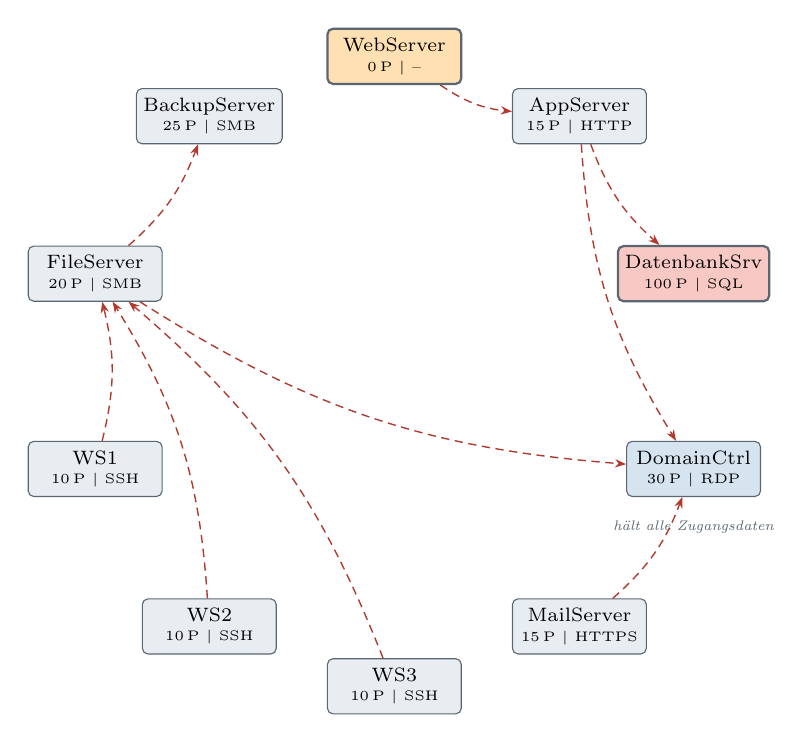
\begin{tikzpicture}[topofig, scale=1.0]
  \node[entrynode] (WebServer) at (0.0,4.0) {WebServer\\[-1pt]{\tiny 0\,P \textbar\ --}};
  \node[netnode] (Workstation1) at (-3.8,-1.24) {WS1\\[-1pt]{\tiny 10\,P \textbar\ SSH}};
  \node[netnode] (Workstation2) at (-2.35,-3.24) {WS2\\[-1pt]{\tiny 10\,P \textbar\ SSH}};
  \node[netnode] (Workstation3) at (0.0,-4.0) {WS3\\[-1pt]{\tiny 10\,P \textbar\ SSH}};
  \node[netnode] (MailServer) at (2.35,-3.24) {MailServer\\[-1pt]{\tiny 15\,P \textbar\ HTTPS}};
  \node[netnode] (FileServer) at (-3.8,1.24) {FileServer\\[-1pt]{\tiny 20\,P \textbar\ SMB}};
  \node[netnode] (AppServer) at (2.35,3.24) {AppServer\\[-1pt]{\tiny 15\,P \textbar\ HTTP}};
  \node[netnode] (BackupServer) at (-2.35,3.24) {BackupServer\\[-1pt]{\tiny 25\,P \textbar\ SMB}};
  \node[dcnode] (DomainController) at (3.8,-1.24) {DomainCtrl\\[-1pt]{\tiny 30\,P \textbar\ RDP}};
  \node[cjnode] (DatabaseServer) at (3.8,1.24) {DatenbankSrv\\[-1pt]{\tiny 100\,P \textbar\ SQL}};
  % Vollstaendiger Graph: alle Kanten wuerden die Abbildung unlesbar
  % machen; stattdessen Hinweis in der Legende.
  \draw[cred] (WebServer) to[bend right=14] (AppServer);
  \draw[cred] (AppServer) to[bend right=14] (DatabaseServer);
  \draw[cred] (AppServer) to[bend right=14] (DomainController);
  \draw[cred] (MailServer) to[bend right=14] (DomainController);
  \draw[cred] (FileServer) to[bend right=14] (BackupServer);
  \draw[cred] (FileServer) to[bend right=14] (DomainController);
  \draw[cred] (Workstation1) to[bend right=14] (FileServer);
  \draw[cred] (Workstation2) to[bend right=14] (FileServer);
  \draw[cred] (Workstation3) to[bend right=14] (FileServer);
  \node[dcbadge, anchor=north] at (3.8,-1.8599999999999999) {h\"alt alle Zugangsdaten};
\end{tikzpicture}
\end{adjustbox}

  \caption[Topologie \emph{flat}]{Topologie \emph{flat}. Die Erreichbarkeit ist
  vollständig, jeder Knoten erreicht jeden anderen; die 90 gerichteten Kanten
  sind nicht eingezeichnet. Dargestellt sind daher nur die Zugangsdaten.}
  \label{fig:topo-flat}
\end{figure}

\paragraph{dmz.}
Die Zuordnung folgt den drei Zonen (\Cref{fig:topo-dmz}). In der
entmilitarisierten Zone liegen der Webserver sowie die beiden Dienste, die er
benötigt: der Mailserver für ausgehende Benachrichtigungen und der
Applikationsserver als Backend. Beide melden sich am Domain-Controller an und
überschreiten damit als einzige die Zonengrenze ins Intranet. Der
Applikationsserver hält zusätzlich die Zugangsdaten der Datenbank, wie es einer
fest konfigurierten Datenbankverbindung entspricht. Im Intranet selbst greift
keine weitere Trennung mehr: Der Domain-Controller erreicht alle Endsysteme,
und der Dateiserver sichert auf den Backup-Server. Genau dieses Gefälle ist
gemeint, wenn vom befestigten Perimeter bei weichem Inneren die Rede ist.

\begin{figure}[H]
  \centering
  % AUTOMATISCH ERZEUGT von gen_topologie_figuren.py -- nicht von Hand aendern.
\begin{adjustbox}{max width=\textwidth}
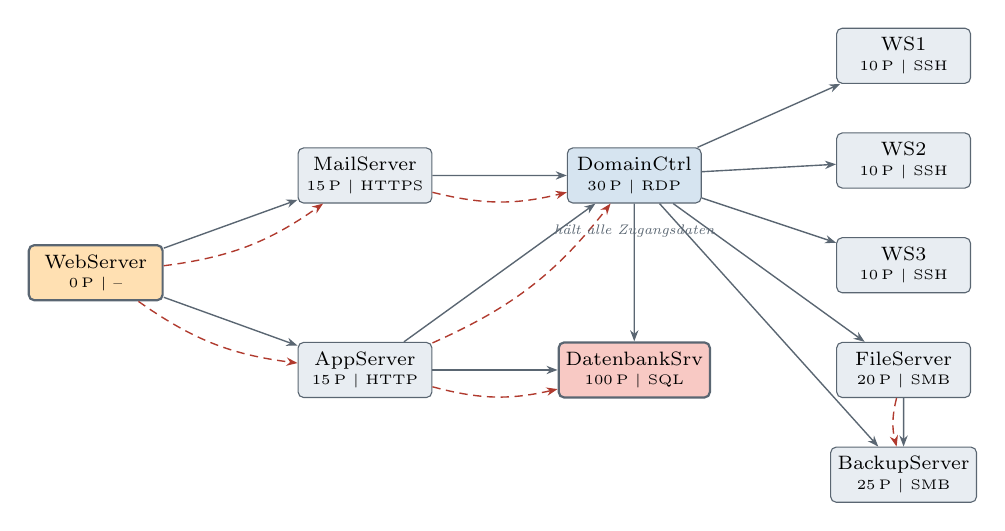
\begin{tikzpicture}[topofig, scale=0.95]
  \node[entrynode] (WebServer) at (0.0,3.1) {WebServer\\[-1pt]{\tiny 0\,P \textbar\ --}};
  \node[netnode] (Workstation1) at (10.8,6.0) {WS1\\[-1pt]{\tiny 10\,P \textbar\ SSH}};
  \node[netnode] (Workstation2) at (10.8,4.6) {WS2\\[-1pt]{\tiny 10\,P \textbar\ SSH}};
  \node[netnode] (Workstation3) at (10.8,3.2) {WS3\\[-1pt]{\tiny 10\,P \textbar\ SSH}};
  \node[netnode] (MailServer) at (3.6,4.4) {MailServer\\[-1pt]{\tiny 15\,P \textbar\ HTTPS}};
  \node[netnode] (FileServer) at (10.8,1.8) {FileServer\\[-1pt]{\tiny 20\,P \textbar\ SMB}};
  \node[netnode] (AppServer) at (3.6,1.8) {AppServer\\[-1pt]{\tiny 15\,P \textbar\ HTTP}};
  \node[netnode] (BackupServer) at (10.8,0.4) {BackupServer\\[-1pt]{\tiny 25\,P \textbar\ SMB}};
  \node[dcnode] (DomainController) at (7.2,4.4) {DomainCtrl\\[-1pt]{\tiny 30\,P \textbar\ RDP}};
  \node[cjnode] (DatabaseServer) at (7.2,1.8) {DatenbankSrv\\[-1pt]{\tiny 100\,P \textbar\ SQL}};
  \draw[reach] (WebServer) -- (MailServer);
  \draw[reach] (WebServer) -- (AppServer);
  \draw[reach] (MailServer) -- (DomainController);
  \draw[reach] (AppServer) -- (DatabaseServer);
  \draw[reach] (AppServer) -- (DomainController);
  \draw[reach] (DomainController) -- (Workstation1);
  \draw[reach] (DomainController) -- (Workstation2);
  \draw[reach] (DomainController) -- (Workstation3);
  \draw[reach] (DomainController) -- (FileServer);
  \draw[reach] (DomainController) -- (BackupServer);
  \draw[reach] (DomainController) -- (DatabaseServer);
  \draw[reach] (FileServer) -- (BackupServer);
  \draw[cred] (WebServer) to[bend right=14] (MailServer);
  \draw[cred] (WebServer) to[bend right=14] (AppServer);
  \draw[cred] (MailServer) to[bend right=14] (DomainController);
  \draw[cred] (AppServer) to[bend right=14] (DatabaseServer);
  \draw[cred] (AppServer) to[bend right=14] (DomainController);
  \draw[cred] (FileServer) to[bend right=14] (BackupServer);
  \node[dcbadge, anchor=north] at (7.2,3.7800000000000002) {h\"alt alle Zugangsdaten};
\end{tikzpicture}
\end{adjustbox}

  \caption[Topologie \emph{dmz}]{Topologie \emph{dmz}. Der Einstiegsknoten
  erreicht nur die beiden Dienste der entmilitarisierten Zone; erst über diese
  führt der Weg ins Intranet.}
  \label{fig:topo-dmz}
\end{figure}

\paragraph{hub\_and\_spoke.}
Die Rolle des Hubs übernimmt der Applikationsserver. Nach dem
Domain-Controller unterhält er die meisten fachlich begründeten Verbindungen
über Bereichsgrenzen hinweg: Er liest aus der Datenbank, meldet sich am
Verzeichnisdienst an und greift auf die Dateiablage zu. Zu den übrigen Spokes
besteht keine solche fachliche Beziehung; die Arbeitsplätze etwa nutzen die
Anwendung über den Webserver und nicht unmittelbar. Das Muster verlangt eine
solche Beziehung aber auch nicht: Die Kanten zwischen Hub und Spokes folgen aus
der Transitrolle selbst, die sämtlichen Verkehr über diesen einen Punkt führt,
und fallen bei jeder Wahl des Hubs gleichermaßen an.

Dass nicht der Domain-Controller zum Hub wurde, obwohl er noch mehr Bereiche
verbindet, ist eine bewusste Entscheidung. Dass der Hub überhaupt ein
übernehmbares System sein muss, ist bereits das oben beschriebene
Zugeständnis an das feste Inventar. Der Domain-Controller hält darüber hinaus
die Zugangsdaten sämtlicher Knoten, und beides zusammen machte seine Übernahme
zum Verlust des gesamten Netzes: Der Angreifer erhielte mit einem einzigen
Knoten Reichweite und Zugriff auf alles, und für sechs der neun übrigen Knoten
verkürzte sich der Angriffsweg um einen Schritt, weil ihre Zugangsdaten dann
bereits am Engpass lägen. Die Trennung von Reichweite und Zugriff, die dieses
Muster gerade auszeichnet, wäre aufgehoben.

Allein der Hub besitzt ausgehende Firewall-Regeln, alle übrigen Knoten haben
keine (\Cref{fig:topo-hub}).

Für den Angreifer bedeutet das eine harte Einschränkung. Von einem übernommenen
Endsystem aus kommt er nicht weiter, denn ein Spoke erreicht keinen anderen
Spoke. Jeder Schritt setzt den Hub voraus. Zugleich verschafft ihm der Hub aber
nur Reichweite, nicht Zugriff: Die Zugangsdaten der Arbeitsplätze sowie des
Mail-, Datei- und Backup-Servers liegen ausschließlich beim Domain-Controller.
Der Angreifer muss also erst diesen übernehmen, um die Reichweite des Hubs
überhaupt nutzen zu können.

\begin{figure}[H]
  \centering
  % AUTOMATISCH ERZEUGT von gen_topologie_figuren.py -- nicht von Hand aendern.
\begin{adjustbox}{max width=\textwidth}
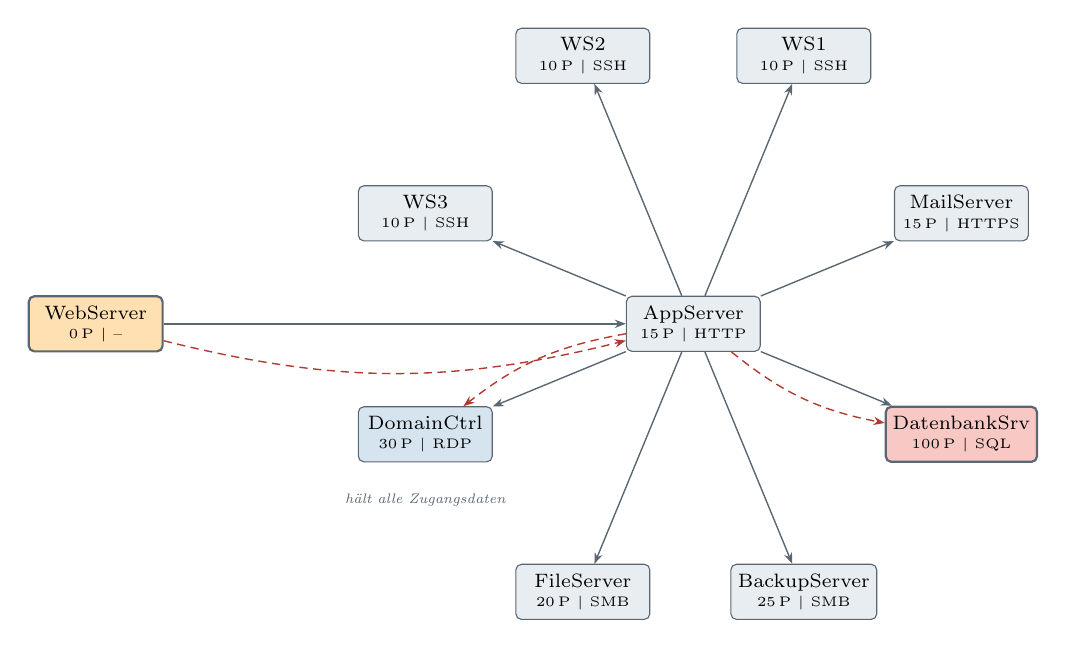
\begin{tikzpicture}[topofig, scale=1.15]
  \node[entrynode] (WebServer) at (-6.6,0.0) {WebServer\\[-1pt]{\tiny 0\,P \textbar\ --}};
  \node[netnode] (Workstation1) at (1.22,2.96) {WS1\\[-1pt]{\tiny 10\,P \textbar\ SSH}};
  \node[netnode] (Workstation2) at (-1.22,2.96) {WS2\\[-1pt]{\tiny 10\,P \textbar\ SSH}};
  \node[netnode] (Workstation3) at (-2.96,1.22) {WS3\\[-1pt]{\tiny 10\,P \textbar\ SSH}};
  \node[netnode] (MailServer) at (2.96,1.22) {MailServer\\[-1pt]{\tiny 15\,P \textbar\ HTTPS}};
  \node[netnode] (FileServer) at (-1.22,-2.96) {FileServer\\[-1pt]{\tiny 20\,P \textbar\ SMB}};
  \node[netnode] (AppServer) at (0.0,0.0) {AppServer\\[-1pt]{\tiny 15\,P \textbar\ HTTP}};
  \node[netnode] (BackupServer) at (1.22,-2.96) {BackupServer\\[-1pt]{\tiny 25\,P \textbar\ SMB}};
  \node[dcnode] (DomainController) at (-2.96,-1.22) {DomainCtrl\\[-1pt]{\tiny 30\,P \textbar\ RDP}};
  \node[cjnode] (DatabaseServer) at (2.96,-1.22) {DatenbankSrv\\[-1pt]{\tiny 100\,P \textbar\ SQL}};
  \draw[reach] (WebServer) -- (AppServer);
  \draw[reach] (AppServer) -- (MailServer);
  \draw[reach] (AppServer) -- (DomainController);
  \draw[reach] (AppServer) -- (Workstation1);
  \draw[reach] (AppServer) -- (Workstation2);
  \draw[reach] (AppServer) -- (Workstation3);
  \draw[reach] (AppServer) -- (FileServer);
  \draw[reach] (AppServer) -- (BackupServer);
  \draw[reach] (AppServer) -- (DatabaseServer);
  \draw[cred] (WebServer) to[bend right=14] (AppServer);
  \draw[cred] (AppServer) to[bend right=14] (DatabaseServer);
  \draw[cred] (AppServer) to[bend right=14] (DomainController);
  \node[dcbadge, anchor=north] at (-2.96,-1.8399999999999999) {h\"alt alle Zugangsdaten};
\end{tikzpicture}
\end{adjustbox}

  \caption[Topologie \emph{hub\_and\_spoke}]{Topologie \emph{hub\_and\_spoke}.
  Der Applikationsserver ist als Hub der einzige Übergang zwischen dem
  Einstiegsknoten und allen übrigen Systemen.}
  \label{fig:topo-hub}
\end{figure}

\paragraph{micro\_segmented.}
Für den Einstiegsknoten bleibt genau eine Verbindung übrig: die zum
Applikationsserver, dessen Backend er als Webserver benötigt. Der
Applikationsserver seinerseits darf die Datenbank und den Domain-Controller
erreichen, weil er Anwendungsdaten liest und Anmeldungen prüfen muss. Zu den
Arbeitsplätzen, zum Mail-, Datei- und Backup-Server besteht dagegen keine
fachliche Notwendigkeit, folglich existiert auch keine entsprechende Freigabe.
Diese sechs Knoten sind damit nicht vom Netz getrennt, sie nehmen ihre Arbeit
weiterhin auf und greifen ihrerseits auf Dienste zu; nach dem oben Gesagten ist
solcher Verkehr hier nur nicht verzeichnet, weil er dem Angreifer keinen Weg
eröffnet. Vom Einstiegsknoten aus führt zu ihnen jedoch kein Pfad, sodass für
den Angreifer höchstens 145 der insgesamt 235 Punkte erreichbar bleiben
(\Cref{fig:topo-micro}).

Ein zweiter Unterschied betrifft die Zugangsdaten und wiegt für den Angriffsweg
schwerer. In den übrigen Topologien hinterlegt der Applikationsserver die
Zugangsdaten der Datenbank dauerhaft bei sich, wie es bei einer fest
konfigurierten Datenbankverbindung üblich ist. Hier speichert er sie nicht; sie
liegen ausschließlich beim Domain-Controller. Der Angreifer erreicht die
Datenbank zwar schon vom Applikationsserver aus, kann sie aber erst übernehmen,
nachdem er den Domain-Controller kompromittiert hat. Aus zwei Sprüngen werden
drei.

\begin{figure}[H]
  \centering
  % AUTOMATISCH ERZEUGT von gen_topologie_figuren.py -- nicht von Hand aendern.
\begin{adjustbox}{max width=\textwidth}
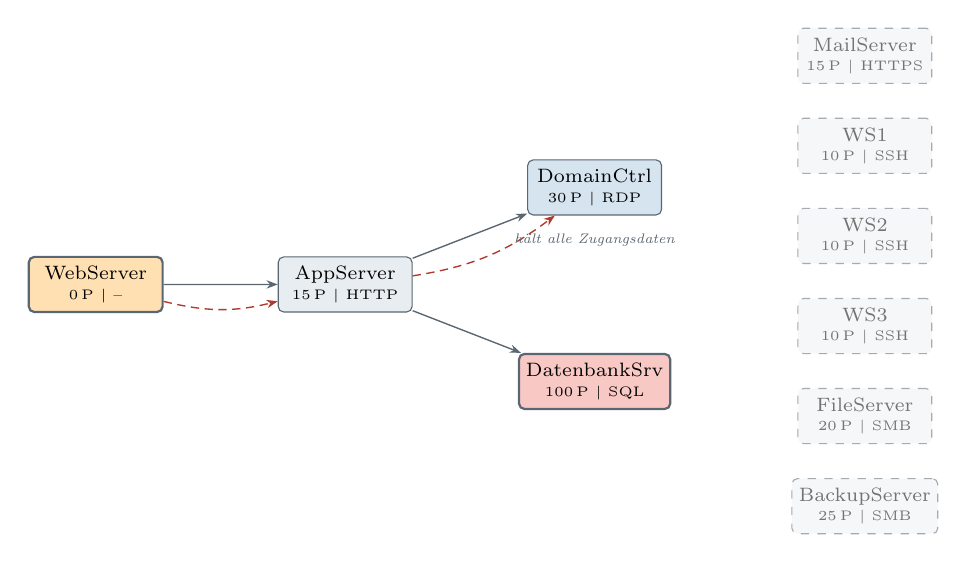
\begin{tikzpicture}[topofig, scale=0.88]
  \node[entrynode] (WebServer) at (0.0,3.2) {WebServer\\[-1pt]{\tiny 0\,P \textbar\ --}};
  \node[netnode,isolated] (Workstation1) at (11.1,5.2) {WS1\\[-1pt]{\tiny 10\,P \textbar\ SSH}};
  \node[netnode,isolated] (Workstation2) at (11.1,3.9) {WS2\\[-1pt]{\tiny 10\,P \textbar\ SSH}};
  \node[netnode,isolated] (Workstation3) at (11.1,2.6) {WS3\\[-1pt]{\tiny 10\,P \textbar\ SSH}};
  \node[netnode,isolated] (MailServer) at (11.1,6.5) {MailServer\\[-1pt]{\tiny 15\,P \textbar\ HTTPS}};
  \node[netnode,isolated] (FileServer) at (11.1,1.3) {FileServer\\[-1pt]{\tiny 20\,P \textbar\ SMB}};
  \node[netnode] (AppServer) at (3.6,3.2) {AppServer\\[-1pt]{\tiny 15\,P \textbar\ HTTP}};
  \node[netnode,isolated] (BackupServer) at (11.1,0.0) {BackupServer\\[-1pt]{\tiny 25\,P \textbar\ SMB}};
  \node[dcnode] (DomainController) at (7.2,4.6) {DomainCtrl\\[-1pt]{\tiny 30\,P \textbar\ RDP}};
  \node[cjnode] (DatabaseServer) at (7.2,1.8) {DatenbankSrv\\[-1pt]{\tiny 100\,P \textbar\ SQL}};
  \draw[reach] (WebServer) -- (AppServer);
  \draw[reach] (AppServer) -- (DatabaseServer);
  \draw[reach] (AppServer) -- (DomainController);
  \draw[cred] (WebServer) to[bend right=14] (AppServer);
  \draw[cred] (AppServer) to[bend right=14] (DomainController);
  \node[dcbadge, anchor=north] at (7.2,3.9799999999999995) {h\"alt alle Zugangsdaten};
\end{tikzpicture}
\end{adjustbox}

  \caption[Topologie \emph{micro\_segmented}]{Topologie
  \emph{micro\_segmented}. Blass dargestellte Knoten sind vom Einstiegsknoten
  aus über keinen Pfad erreichbar. Anders als in den übrigen Topologien
  speichert der Applikationsserver die Zugangsdaten der Datenbank
  nicht zwischen; sie liegen ausschließlich beim Domain-Controller.}
  \label{fig:topo-micro}
\end{figure}

\paragraph{chain.}
Die Kette ist als strikte Linie ohne jede Verzweigung ausgelegt
(\Cref{fig:topo-chain}) und damit die einfachste denkbare Anordnung: Wer sie
lösen will, muss nur den Nachbarn entdecken, dessen Zugangsdaten auslesen und
ihn übernehmen, und das neun Mal hintereinander. Ein darauf trainierter
Angreifer beherrscht folglich genau dieses Grundmuster und nichts darüber
hinaus, insbesondere keine Entscheidung zwischen mehreren Wegen.

Damit dient die Kette als Kontrollbedingung für die Frage, ob dieses
Grundmuster allein bereits genügt. Behauptet sich ein solcher Angreifer auch in
den vier verzweigten Topologien, spricht das dafür, dass diese sich für den
Verteidiger weniger unterscheiden, als ihre Struktur nahelegt. Scheitert er
dort, lässt sich umgekehrt annehmen, dass die Verzweigungen eine andere
Fähigkeit verlangen. Ein Beweis ist beides nicht, da nur eine einzelne
Angreiferherkunft betrachtet wird; als Anhaltspunkt taugt der Vergleich
gleichwohl. Voraussetzung dafür ist, dass auch der Kette dasselbe Inventar
zugrunde liegt: dieselben zehn Knoten, dieselben Werte, dieselben
Zugangsports. Verändert ist allein die Anordnung.

\begin{figure}[H]
  \centering
  % AUTOMATISCH ERZEUGT von gen_topologie_figuren.py -- nicht von Hand aendern.
\begin{adjustbox}{max width=\textwidth}
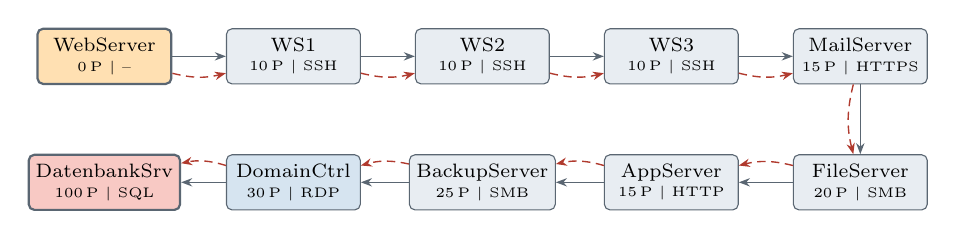
\begin{tikzpicture}[topofig, scale=1.0]
  \node[entrynode] (WebServer) at (0.0,1.6) {WebServer\\[-1pt]{\tiny 0\,P \textbar\ --}};
  \node[netnode] (Workstation1) at (2.4,1.6) {WS1\\[-1pt]{\tiny 10\,P \textbar\ SSH}};
  \node[netnode] (Workstation2) at (4.8,1.6) {WS2\\[-1pt]{\tiny 10\,P \textbar\ SSH}};
  \node[netnode] (Workstation3) at (7.2,1.6) {WS3\\[-1pt]{\tiny 10\,P \textbar\ SSH}};
  \node[netnode] (MailServer) at (9.6,1.6) {MailServer\\[-1pt]{\tiny 15\,P \textbar\ HTTPS}};
  \node[netnode] (FileServer) at (9.6,0.0) {FileServer\\[-1pt]{\tiny 20\,P \textbar\ SMB}};
  \node[netnode] (AppServer) at (7.2,0.0) {AppServer\\[-1pt]{\tiny 15\,P \textbar\ HTTP}};
  \node[netnode] (BackupServer) at (4.8,0.0) {BackupServer\\[-1pt]{\tiny 25\,P \textbar\ SMB}};
  \node[dcnode] (DomainController) at (2.4,0.0) {DomainCtrl\\[-1pt]{\tiny 30\,P \textbar\ RDP}};
  \node[cjnode] (DatabaseServer) at (0.0,0.0) {DatenbankSrv\\[-1pt]{\tiny 100\,P \textbar\ SQL}};
  \draw[reach] (WebServer) -- (Workstation1);
  \draw[reach] (Workstation1) -- (Workstation2);
  \draw[reach] (Workstation2) -- (Workstation3);
  \draw[reach] (Workstation3) -- (MailServer);
  \draw[reach] (MailServer) -- (FileServer);
  \draw[reach] (FileServer) -- (AppServer);
  \draw[reach] (AppServer) -- (BackupServer);
  \draw[reach] (BackupServer) -- (DomainController);
  \draw[reach] (DomainController) -- (DatabaseServer);
  \draw[cred] (WebServer) to[bend right=14] (Workstation1);
  \draw[cred] (Workstation1) to[bend right=14] (Workstation2);
  \draw[cred] (Workstation2) to[bend right=14] (Workstation3);
  \draw[cred] (Workstation3) to[bend right=14] (MailServer);
  \draw[cred] (MailServer) to[bend right=14] (FileServer);
  \draw[cred] (FileServer) to[bend right=14] (AppServer);
  \draw[cred] (AppServer) to[bend right=14] (BackupServer);
  \draw[cred] (BackupServer) to[bend right=14] (DomainController);
  \draw[cred] (DomainController) to[bend right=14] (DatabaseServer);
\end{tikzpicture}
\end{adjustbox}

  \caption[Topologie \emph{chain}]{Topologie \emph{chain}, verwendet für das
  Angreifertraining. Jeder Knoten gibt Erreichbarkeit und Zugangsdaten
  ausschließlich für seinen Nachfolger preis; von dieser Topologie führen neun
  Sprünge bis zum Crown Jewel.}
  \label{fig:topo-chain}
\end{figure}

\section{Trainingsphasen}
\label{sec:phasen}

Der Versuch gliedert sich in zwei Phasen. In der ersten wird ausschließlich der
Angreifer trainiert, in der zweiten ausschließlich der Verteidiger.

\subsection{Phase 1: Angreifer-Vortraining}

Ein Verteidiger lässt sich nur sinnvoll bewerten, wenn ihm ein kompetenter
Gegner gegenübersteht. Deshalb werden zunächst Angreifer ohne jede Verteidigung
trainiert, jeweils \num{500000} Zeitschritte lang.

Naheliegend wäre, den Angreifer schon hier gegen einen Verteidiger antreten zu
lassen, etwa einen zufällig handelnden, um ihn auf spätere Gegenwehr
vorzubereiten. Darauf wird bewusst verzichtet, und zwar aus demselben Grund, aus
dem in Phase~2 der Angreifer eingefroren wird: Was den Angreifer formt, soll
allein die Topologie sein. Ein mittrainierter Verteidiger, ob zufällig oder
lernend, wirkt als zweite Einflussgröße auf die Herkunft jedes Angreifers ein,
und die beobachteten Unterschiede zwischen den Angreifern ließen sich nicht mehr
eindeutig der Struktur zuschreiben. Ein zufälliger Verteidiger wäre zudem selbst
willkürlich gesetzt: Seine Aktionen bevorzugten keine Topologie planvoll,
verzerrten das Angreifertraining aber dennoch in einer nicht kontrollierten
Weise. Der Preis dieser Reinheit ist, dass die Angreifer keine Erfahrung mit
Gegenwehr sammeln; \Cref{sec:limitationen} greift das auf.

Fünf \emph{Spezialisten} entstehen dabei, einer je Topologie. Jeder lernt zwar
nur in einer einzigen Umgebung, tritt in Phase~2 jedoch in allen vier
Verteidigungstopologien als Gegner an. Ein Angreifer trifft dort also in aller
Regel auf eine Struktur, die er im Training nicht gesehen hat. Genau diese
Kreuzung erlaubt es, den Einfluss der verteidigten Topologie von dem der
Angreiferherkunft zu trennen. Ergänzend
wird ein \emph{Generalist} trainiert, im Folgenden Super-Angreifer genannt: Ein
einzelnes Modell durchläuft nacheinander alle fünf Topologien -- in der
Reihenfolge \emph{chain}, \emph{flat}, \emph{hub\_and\_spoke}, \emph{dmz},
\emph{micro\_segmented} --, wobei die Gewichte von Stufe zu Stufe
weitergereicht werden. Damit lässt sich prüfen, ob
ein über mehrere Strukturen trainierter Angreifer den Spezialisten überlegen
ist.

\subsection{Phase 2: Verteidiger-Matrix}

In der zweiten Phase wird für jede Kombination aus Verteidigungstopologie und
Angreifer ein eigener Verteidiger trainiert. Bei vier Topologien und sechs
Angreifern ergeben sich 24~Matchups. Der Angreifer ist dabei \emph{eingefroren}:
Sein Modell wird geladen, handelt weiter, erhält aber keine Gewichtsanpassungen
mehr.

Das Einfrieren hält den Gegner über den gesamten Lauf konstant und macht die
beobachtete Lernkurve dem Verteidiger zurechenbar. Lernten beide Agenten
gleichzeitig, verschöbe sich das Ziel fortlaufend, und ein Unterschied zwischen
zwei Topologien ließe sich nicht mehr von einem Unterschied im Gegnerverhalten
trennen. Diese Entscheidung lässt sich auch am MARLon-Aufbau selbst
festmachen: Dort führt gleichzeitiges Training beider Agenten dazu, dass der
Angreifer keinen brauchbaren Angriffsweg mehr findet, weil wiederholte
Rücksetzungen durch einen anfangs instabilen Verteidiger ihn immer wieder auf
den Ausgangszustand zurückwerfen, bevor er über den Anfang der Episode
hinauskommt~\autocite{marlon}. Erkauft wird die Zurechenbarkeit damit, dass der
Verteidiger sich auf genau ein unveränderliches Gegnerverhalten einspielen kann.
Eben deshalb wird nicht ein einzelner Angreifer eingesetzt, sondern gegen jede
Topologie alle sechs: Jeder Verteidiger sieht zwar nur einen Gegner, über die
Matrix hinweg werden aber sechs verschiedene Angriffsmuster geprüft, davon fünf,
die nicht auf der verteidigten Topologie entstanden sind. Vollständig aufheben
lässt sich die Einschränkung dadurch nicht; \Cref{sec:limitationen} greift sie auf.

Jedes Matchup wird fünfmal wiederholt, und verglichen wird nicht der einzelne
Lauf, sondern der über die fünf Wiederholungen gemittelte Verlauf. Insgesamt
ergeben sich damit \num{120}~Trainingsläufe zu je \num{500000} Zeitschritten.

\section{Aktionsraum und Invalid-Action-Masking}
\label{sec:masking}

Was ein Agent lernen kann, ist durch die Menge der ihm zur Verfügung
stehenden Aktionen begrenzt. Dieser Abschnitt beschreibt diese Menge für
beide Seiten samt der Maskierung, die im jeweiligen Zustand ungültige
Aktionen ausschließt, und prüft abschließend, welche mehrstufigen
Strategien darin überhaupt angelegt sind.

\subsection{Der Aktionsraum des Angreifers}
\label{sec:aktionsraum-atk}

In jedem Zeitschritt wählt der Angreifer genau eine Aktion aus. Eine Aktion ist
dabei keine grobe Absicht wie \glqq greife den Dateiserver an\grqq{}, sondern eine
vollständig ausformulierte Anweisung: Sie legt fest, was getan wird, von
welchem Knoten aus und gegen welches Ziel. \ac{CBS} kennt dafür drei Arten.

Eine \emph{lokale Aktion} durchsucht einen bereits übernommenen Knoten von
innen, etwa nach dort gespeicherten Zugangsdaten. Eine \emph{entfernte Aktion}
richtet sich von einem übernommenen Knoten aus gegen ein anderes System und
späht dieses aus. Eine \emph{Verbindung} meldet sich mit erbeuteten
Zugangsdaten an einem Zielknoten an und übernimmt ihn. Nur die dritte Art
erweitert den Besitz; die ersten beiden beschaffen die Voraussetzungen dafür.

Jede Kombination aus Aktionsart und Parametern bildet einen eigenen Eintrag.
Die Größe des Aktionsraums ergibt sich damit als Produkt der jeweiligen
Auswahlmöglichkeiten (\Cref{tab:aktionsraum}).

\begin{table}[H]
  \centering
  \caption[Aufbau des Aktionsraums]{Aufbau des Aktionsraums des Angreifers bei
  zehn Knoten.}
  \label{tab:aktionsraum}
  \begin{tabular}{llr}
    \toprule
    Art & Parameter & Anzahl \\
    \midrule
    Lokale Aktion   & 10 Knoten $\times$ 2 Schwachstellen & 20 \\
    Entfernte Aktion & 10 Quellen $\times$ 10 Ziele $\times$ 1 Schwachstelle & 100 \\
    Verbindung      & 10 Quellen $\times$ 10 Ziele $\times$ 6 Ports $\times$ 9 Zugangsdaten & 5400 \\
    \midrule
    Gesamt          &  & 5520 \\
    \bottomrule
  \end{tabular}
\end{table}

Die 5400 Verbindungen wirken auf den ersten Blick redundant, denn ein Knoten
besitzt in der Modellierung genau einen Zugangsport und genau einen Satz
Zugangsdaten; mit der Wahl des Ziels stünden beide inhaltlich also bereits
fest. \ac{CBS} nimmt diese Einschränkung jedoch nicht vor:
Angeboten werden für jede Quelle-Ziel-Kombination sämtliche 54 Kombinationen
aus Port und zwischengespeicherter Zugangsdatenkarte, mit dem ausdrücklichen
Hinweis im Quellcode der Umgebung, dass Erfolg damit nicht garantiert sei. Der
Angreifer muss also selbst lernen, welche einzelne davon zum jeweiligen Knoten
passt; sie sind dem Aktionsraum nicht vorweg entzogen.

Technisch sind diese 5520 Einträge als flaches \texttt{Discrete} umgesetzt,
also als eine einzige durchnummerierte Liste, in der jede vollständige Aktion
einen eigenen Index besitzt. MARLon verwendet an dieser Stelle ein
\texttt{MultiDiscrete}, bei dem der Agent je Zug eine Reihe von Zahlen ausgibt:
eine für die Aktionsart, weitere für Quellknoten, Zielknoten, Port und
Zugangsdaten.

Nötig wurde die Umstellung durch das im Folgenden beschriebene Masking. Dieses
kennzeichnet jeden Eintrag der Liste einzeln als gültig oder ungültig. Bei einem
\texttt{MultiDiscrete} müsste jede Stelle für sich gekennzeichnet werden, und
damit lassen sich verknüpfte Bedingungen nicht ausdrücken: Ob ein Zielknoten in
Frage kommt, hängt davon ab, welcher Quellknoten gewählt wurde, denn nur von
einem übernommenen Knoten aus lässt sich überhaupt handeln. Eine Kennzeichnung
je Stelle kennt diese Abhängigkeit nicht und müsste einen Zielknoten entweder
immer oder nie zulassen. Erst wenn sämtliche Kombinationen als einzelne
Einträge nebeneinanderstehen, lässt sich die Bedingung abbilden, weil dann genau
die gültigen \emph{Gesamt}aktionen bezeichnet werden können. Der Preis ist eine
sehr lange Liste, doch da davon je Schritt nur wenige Einträge gültig sind,
wählt der Angreifer tatsächlich aus einer kleinen Menge.

Das Verfahren selbst ist das \emph{Invalid-Action-Masking} nach Huang und
Ontañón~\autocite{huang2022masking}. Vor jeder Entscheidung wird
ein boolescher Vektor übergeben, der die im aktuellen Zustand gültigen Aktionen
markiert; die Policy wählt ausschließlich aus diesen. Ohne Maskierung entfällt
ein Großteil der Schritte auf wirkungslose Aktionen, etwa den Angriff von einem
nicht kontrollierten Knoten aus.

Technisch gibt der Actor je Aktion zunächst einen unnormierten Zahlenwert aus,
ein sogenanntes \emph{Logit}; erst ein nachgelagerter Rechenschritt überführt
diese Werte in die Wahrscheinlichkeiten der
Policy~\cite[Abschn.~\glqq Background\grqq{}]{huang2022masking}. Die Maskierung
setzt an dieser Stelle an: Die Logits ungültiger Aktionen werden vor der
Normierung durch eine sehr große negative Zahl ersetzt, in der hier
eingesetzten Implementierung $-10^{8}$, sodass ihre Wahrscheinlichkeit
praktisch null wird. Die Wahrscheinlichkeitsmasse verteilt sich dadurch
ausschließlich auf die gültigen Aktionen, statt über alle 5520 zu streuen. Die
Markov-Eigenschaft bleibt davon unberührt, denn maskiert wird nicht der Zustand,
sondern die in ihm zulässige Aktionsmenge. Zustandsabhängige Aktionsmengen sind
Bestandteil der üblichen \ac{MDP}-Definition. Huang und Ontañón zeigen zudem,
dass der resultierende Gradient weiterhin ein gültiger Policy-Gradient
ist~\autocite{huang2022masking}.

Entscheidend ist der Zeitpunkt der Maskenberechnung. Sie erfolgt unmittelbar
vor der Aktionswahl aus dem aktuellen Zustand. Eine zwischengespeicherte Maske
wäre um den vorangegangenen Verteidigerzug veraltet, da dieser Knoten neu
aufsetzen oder Verbindungen sperren kann. Huang und Ontañón behandeln den Fall
eines einzelnen Agenten, bei dem diese Frage nicht auftritt; sobald ein zweiter
Agent zwischen zwei Zügen handelt, genügt es nicht mehr, die Maske einmal je
eigenem Schritt zu bestimmen.

\subsubsection{Reichweite der Maskierung: Zugangsdaten allein genügen nicht}
\label{sec:mask-reichweite}

Die von \ac{CBS} bereitgestellte Aktionsmaske prüft für eine Verbindung
ausschließlich, ob der Angreifer die betreffende Zugangsdatenkarte besitzt,
nicht aber, ob zwischen Quelle und Ziel überhaupt ein Netzpfad besteht.
Weil die Modellierung Erreichbarkeit und Zugangsdatenbesitz trennt
(\Cref{sec:topomodell}), würde sie damit Verbindungen entlang gar nicht
vorhandener Kanten erlauben, sobald der Angreifer die passenden
Zugangsdaten irgendwo erbeutet hat, und die Topologie als Einflussgröße
unterlaufen.

Die native Maske wurde deshalb um eine eigene Einschränkung ergänzt. Der Angreifer führt seither mit, welche Kante er von welchem Knoten aus
tatsächlich aufgedeckt hat; aufgedeckt wird eine Kante ausschließlich durch
die auf den Quellknoten gerichtete lokale Aktion zur
Nachbarschaftserkundung, nicht durch das Erbeuten von Zugangsdaten. Die von
\ac{CBS} gelieferte Maske wird für Verbindungen und entfernte Aktionen mit
dieser Liste geschnitten und bildet damit auch die Netzstruktur ab.

Anders als das Masking selbst, das bereits im Referenzlauf eingesetzt wurde,
stammt diese Erweiterung aus der späteren Überarbeitung. Sie greift unmittelbar
in das Verhalten des Angreifers ein, weshalb sämtliche Angreifer für die
berichteten Läufe neu vortrainiert wurden.

\subsection{Der Aktionsraum des Verteidigers}
\label{sec:aktionsraum-def}

Der Verteidiger verfügt über drei Aktionsarten: Er kann einen Knoten \emph{neu
aufsetzen} und damit den Angreifer von diesem System vertreiben, er kann
dessen eingehenden \emph{Verkehr sperren}, und er kann eine bestehende Sperre
wieder \emph{aufheben}. Jede der drei Arten benennt ausschließlich den
betroffenen Knoten; Sperren und Aufheben wirken dabei auf sämtliche
eingehenden Dienste dieses Knotens zugleich, ohne dass Port oder Richtung
gesondert gewählt würden.

Technisch ist das als \texttt{MultiDiscrete} über vier Dimensionen umgesetzt,
$[3, 10, 10, 10]$. Der erste Wert wählt die Aktionsart, die übrigen drei
benennen den Knoten für Neuaufsetzen, Sperren beziehungsweise Aufheben; nur
die zur gewählten Art passende Dimension wird ausgewertet
(\Cref{tab:aktionsraum-def}).

\begin{table}[H]
  \centering
  \caption[Aktionsraum des Verteidigers]{Aktionsraum des Verteidigers bei zehn
  Knoten.}
  \label{tab:aktionsraum-def}
  \begin{tabular}{llrr}
    \toprule
    Aktionsart & Parameter & Kombinationen & davon wirksam \\
    \midrule
    Knoten neu aufsetzen & 10 Knoten & 10 & 9 \\
    Verkehr sperren      & 10 Knoten & 10 & 9 \\
    Verkehr aufheben     & 10 Knoten & 10 & 9 \\
    \midrule
    Gesamt                &  & 30 & 27 \\
    \bottomrule
  \end{tabular}
\end{table}

Der Einstiegsknoten schränkt beide Spalten der Tabelle zusätzlich ein. Er ist
nicht neu aufsetzbar, wodurch für das Neuaufsetzen nur neun der zehn Knoten
tatsächlich gültige Ziele sind. Eine Sperre auf ihm ist zwar technisch gültig,
bringt aber nie einen Nutzen: Er trägt den Wert null und bleibt über die
gesamte Episode kompromittiert, weil er nicht zurückgewonnen werden kann.
Wirksam wählbar bleiben damit 27 der 30 strukturell möglichen Aktionen.

Gegenüber dem Original ist dieser Aktionsraum damit in zweifacher Hinsicht
enger. MARLon sieht fünf Aktionsarten vor, neben dem Neuaufsetzen, dem Sperren
und dem Aufheben auch das Stoppen und das Starten eines Dienstes, und verlangt
zu jeder von ihnen zusätzlich Port und Richtung als selbst zu wählende
Parameter (\Cref{sec:marlon-original}). Hier sind es drei Aktionsarten mit dem
Knoten als einzigem Parameter. Beide Änderungen gehen auf Beobachtungen am
Referenzlauf zurück.

Als erste Änderung sind Dienst stoppen und Dienst starten entfallen. Für den Angreifer ist
ein gestoppter Dienst von einer gesperrten Verbindung ohnehin nicht zu
unterscheiden, beide lassen den Verbindungsversuch scheitern. Da eine Sperre
nach dem Umbau denselben Knoten in seiner Gesamtheit betrifft und seit der in
\Cref{sec:sla} beschriebenen Korrektur ebenfalls Verfügbarkeit kostet, blieb
kein Zweck, den nicht auch sie erfüllt.

Ausschlaggebend war damit nicht, dass eine der beiden Aktionen die schlechtere
gewesen wäre, sondern dass zwei Aktionen für dieselbe Wirkung den Aktionsraum
ohne Gewinn an Ausdruckskraft vergrößert hätten. Dass die Wahl auf die Sperre
fiel, hat einen inhaltlichen Grund: Sie setzt am Zugang zu einem System an und
lässt dessen Betrieb unberührt, während ein Dienststopp in das System selbst
eingreift. Von zwei gleich wirkenden Mitteln ist damit das mildere gewählt.

Offenzulegen ist dabei, dass diese Gleichwertigkeit nur für die Sperre in ihrer
heutigen Form gilt und nie gemessen wurde. Im Referenzlauf standen dem
Verteidiger zwar beide Aktionen gleichzeitig zur Verfügung, aber nicht als
gleichwertige Alternativen: Die Sperre wirkte dort je Port statt je Knoten,
erreichte wegen der in \Cref{sec:marlon-fehler} beschriebenen Portliste die
wertvollsten Systeme überhaupt nicht und brachte, da sie weder Verfügbarkeit
kostete noch belohnt wurde, keinerlei Signal hervor. Der Dienststopp dagegen
war auf sauberen Knoten mit zehn Punkten belastet. Dass der Verteidiger ihn
dort ablegte, ist deshalb kein Vergleichsergebnis. Ein Lauf, in dem beide
Aktionen unter den heutigen Bedingungen nebeneinander zur Wahl stünden, wurde
nicht durchgeführt; die Gleichwertigkeit folgt aus der Betrachtung der
Wirkungsketten, nicht aus einer Messung.

Als zweite Änderung wählt der Verteidiger für Sperren und Freigaben nicht mehr selbst,
welcher Port betroffen ist. Er benennt nur den Knoten; welche Dienste dort
laufen, ist als Grundwissen des Betreibers vorausgesetzt und kein
Erkundungsergebnis, wie es für den Angreifer eines wäre. Dieselbe Asymmetrie
gilt bereits an anderer Stelle des Modells: Der Verteidiger spricht jeden
Knoten direkt über seinen Index an und darf ihn neu aufsetzen, sieht sein
eigenes Netz für die Zwecke dieser Aktionen also vollständig. Die Wahl des
Ports blieb die einzige Stelle, an der er über sein eigenes Netz raten musste;
diese Uneinheitlichkeit ist mit der Änderung beseitigt.

\subsection{Mehrstufige Strategien im Aktionsraum}
\label{sec:mehrstufig}

Die Wirkung einer Verteidigeraktion hängt davon ab, wo sie ansetzt. Eine
Sperre wirkt nur auf den \emph{Ziel}knoten einer Verbindung. Auf einem Knoten,
den der Angreifer bereits besitzt, ändert eine Sperre deshalb nichts, denn als
Ausgangspunkt einer weiteren Verbindung braucht er den eigenen eingehenden
Zugang nicht. Auf einem noch nicht übernommenen Knoten verhindert sie die
Übernahme über diesen Weg sehr wohl.

Daraus folgt eine Strategie, die den Angreifer vollständig einschließen würde:
Man drängt ihn durch wiederholtes Neuaufsetzen auf den Einstiegsknoten zurück
und sperrt anschließend alle von dort aus erreichbaren Knoten. Der Angreifer
besäße dann zwar weiterhin ein System, käme aber nirgendwo mehr hin. Der
Aktionsraum sieht diese Möglichkeit demnach vor.

Ob ein lernendes Verfahren sie auch findet, ist eine andere Frage. Die
Einschließung besteht aus vielen einzelnen Sperren, und ihr Nutzen tritt erst
ein, wenn die letzte von ihnen gesetzt ist: Solange auch nur ein Weg offen
bleibt, nimmt der Angreifer ihn. Bis dahin bringt jede einzelne Sperre für sich
genommen nichts. Der Verteidiger müsste eine lange Folge bestimmter Aktionen
zufällig treffen, bevor sich überhaupt ein Reward zeigt, an dem \ac{PPO} sie
erkennen könnte. Das ist der in \Cref{sec:credit} beschriebene Fall der
verzögerten Belohnung in ausgeprägter Form.

Erreichbar wird eine solche Strategie erst, wenn bereits die einzelne Sperre
einen eigenen Reward trägt, wenn die Zwischenschritte also für sich verstärkt
werden und der Agent sie nicht erst am Ende der Kette bewertet bekommt. Genau
darauf zielt der in \Cref{sec:abwehrbonus} beschriebene Abwehrbonus. Ob er
dafür ausreicht, wird in \Cref{ch:ergebnisse} untersucht.

\section{Reward-Struktur und Randbedingungen}
\label{sec:rewards}

Der Reward entsteht auf zwei Ebenen: \ac{CBS} bewertet jede Angreiferaktion,
und der Wrapper setzt darauf die Kopplung beider Agenten sowie die in diesem
Abschnitt beschriebenen Ergänzungen.

\begin{longtable}{EWK}
    \caption[Reward des Angreifers]{Reward des Angreifers je Aktion. Aufgeführt
    sind nur die Bestandteile, die in den hier verwendeten Topologien überhaupt
    auftreten können. Der untere Block stammt nicht aus \ac{CBS}, sondern wird
    vom Wrapper ergänzt.}
    \label{tab:reward-atk} \\
    \toprule
    Ereignis & Reward & Anmerkung \\
    \midrule
    \endfirsthead
    \toprule
    Ereignis & Reward & Anmerkung \\
    \midrule
    \endhead
    \midrule
    \multicolumn{3}{@{}r@{}}{\footnotesize Fortsetzung auf der nächsten Seite} \\
    \endfoot
    \bottomrule
    \endlastfoot
    Knoten übernommen             & $+$Knotenwert & 10 bis 100, auch nach Rückeroberung \\
    Knoten neu entdeckt           & $+5$  & je Knoten \\
    Zugangsdaten neu entdeckt     & $+3$  & je Credential \\
    Eigenschaft neu entdeckt      & $+2$  & je Eigenschaft eines Knotens, hier Betriebssystem und Rolle, die ein Scan aus der Ferne sichtbar macht \\
    Aktion erstmals erfolgreich   & $+7$  & je Knoten und Schwachstelle \\
    Fehlversuch, Wiederholung, Aktionskosten & $0$ & in \ac{CBS} zwischen $-1$ und $-50$, durch die unten beschriebene Kappung ohne Wirkung \\
    Alle Knoten übernommen        & $+5000$ & ersetzt den Schrittwert \\
    \midrule
    Knoten gehalten               & $+0{,}005\cdot$Knotenwert & je Knoten und Schritt \\
    Knoten durch Reimage verloren & $-$Knotenwert & \\
\end{longtable}

Damit ist der Reward des Angreifers vollständig beschrieben. Der des
Verteidigers folgt in \Cref{tab:reward-def}. Er entsteht überwiegend durch
Spiegelung der eben aufgeführten Werte und trägt darüber hinaus einige eigene
Posten.

\begin{longtable}{EWK}
    \caption[Reward des Verteidigers]{Reward des Verteidigers je Schritt.}
    \label{tab:reward-def} \\
    \toprule
    Ereignis & Reward & Anmerkung \\
    \midrule
    \endfirsthead
    \toprule
    Ereignis & Reward & Anmerkung \\
    \midrule
    \endhead
    \midrule
    \multicolumn{3}{@{}r@{}}{\footnotesize Fortsetzung auf der nächsten Seite} \\
    \endfoot
    \bottomrule
    \endlastfoot
    Grundkopplung             & $-$Angreifer-Reward & jeder Schritt \\
    Abwehrbonus & $\pm 0{,}00025\cdot$Knotenwert & je Knoten, der gesperrt und zugleich nicht kompromittiert ist; Vorzeichen je nach Bedrohungslage, \Cref{sec:abwehrbonus} \\
    Ungültige Aktion          & $0$ & Zug wird übersprungen \\
    \midrule
    \ac{SLA} unterschritten   & $-50$ & je Schritt, ergänzt den Schrittwert \\
    Angreifer vollständig entfernt & $+5000$ & strukturell unerreichbar \\
\end{longtable}

Mehrere Eigenschaften dieser Struktur sind für die Auswertung wesentlich und
nicht offensichtlich.

Erstens erklärt sich die Nullzeile in \Cref{tab:reward-atk} aus einer Kappung:
\ac{CBS} kennt für Fehlversuche, Wiederholungen und Aktionskosten durchaus
Abzüge, begrenzt den Schrittwert des Angreifers aber nach unten auf null, bevor
er zurückgegeben wird. Ein Fehlversuch kostet ihn also nichts, er bringt
lediglich nichts ein. Diese Kappung ist für sich genommen
sinnvoll: Sie verhindert, dass der Verteidiger über die Grundkopplung Reward
für Vorgänge gutgeschrieben bekäme, zu denen er nichts beigetragen hat, was
das Lernsignal verfälschen würde. Sie schließt aber zugleich, in Verbindung mit
der reinen Grundkopplung, den Kanal, über den Prävention im Reward sichtbar
würde, wie \Cref{sec:marlon-original} gezeigt hat. Die Begrenzung greift
zudem nur auf dem Wert, den \ac{CBS} selbst berechnet; der untere
Tabellenblock wird erst danach aufgeschlagen. Negative Angreifer-Rewards
entstehen deshalb ausschließlich durch verlorene Knoten: Setzt der
Verteidiger einen übernommenen Knoten neu auf, verliert der Angreifer dessen
Wert.

Zweitens folgt aus dem Abzug für verlorene Knoten eine Bedingung, die \ac{CBS}
von sich aus nicht erfüllt. Der Abzug ist eine eigene Ergänzung
(\Cref{tab:reward-atk}, unterer Block): Im Auslieferungszustand kostet ein
Reimage den Angreifer nichts, er behält den einmal gutgeschriebenen Knotenwert
einfach. Damit ist dort auch nichts unausgeglichen. Sobald ein Verlust aber
etwas kostet, muss die Rückeroberung desselben Knotens ihn wieder einbringen,
sonst ist der Kreislauf aus Verlust und Rückeroberung kein Nullsummengeschäft
mehr.

Genau hier lag die Ursache des in \Cref{sec:referenzlauf} geschilderten
Verhaltens, das dem Referenzlauf vorausging. \ac{CBS} schreibt einen Knotenwert
nur beim \emph{ersten} Besitz gut und vermerkt die Übernahme dauerhaft; ein
Reimage löscht diesen Vermerk nicht. Zusammen mit dem neu eingeführten Abzug
erhielt der Angreifer für eine Rückeroberung also nichts, während ihn jeder
Verlust den vollen Knotenwert kostete. Über die Grundkopplung wurde daraus eine
Einnahmequelle für den Verteidiger: Er konnte denselben Knoten wieder und
wieder neu aufsetzen und dabei jedes Mal dessen Wert vereinnahmen, ohne dass
sich an der Lage im Netz etwas änderte. In Vorversuchen trat dieses Verhalten
deutlich hervor. Bei zehn vorhandenen Knoten wurden bis zu 268 Rückgewinnungen
je Episode gezählt, und der Verteidiger-Reward korrelierte mit der Zahl der
Reimages bis zu $r = +0{,}98$. Der Vermerk wird beim Verlust eines Knotens
deshalb zurückgesetzt. Jede Rückeroberung zählt damit erneut als erste und
gleicht den vorangegangenen Abzug exakt aus. Der Verteidiger behält seinen
Gewinn nur dann, wenn der Angreifer den Knoten nicht zurückholt.

Drittens maß der Reward vor der hier vorgenommenen Ergänzung nur, \emph{ob}
ein Knoten kompromittiert wurde, nicht \emph{wie lange}. Ein Angreifer, der ein
System zwei Schritte lang hielt, stand damit genauso da wie einer, der es über
die gesamte Episode behielt. Der Schaden eines kompromittierten Systems hängt
jedoch von beidem ab: von seinem Wert und von der Verweildauer des Angreifers.
Deshalb erhält der Angreifer je Schritt einen Anteil des Werts aller aktuell
gehaltenen Knoten. Ein fester Betrag je Knoten würde
Arbeitsplatz\-rechner und Produktionsdatenbank gleichsetzen; der wertanteilige Bonus tut das
nicht, und der Einstiegsknoten mit dem Wert null fällt automatisch heraus.

Über die Grundkopplung wirkt dieser Haltebonus unmittelbar auf den
Verteidiger, der damit nicht nur für die Rückeroberung belohnt wird, sondern
auch dafür, sie früh zu erreichen. Genau diese Kopplung bestimmt auch die
Größenordnung des in \Cref{sec:abwehrbonus} eingeführten Abwehrbonus. Der
Verteidiger steht bei einem kompromittierten Knoten stets vor der Wahl,
diesen neu aufzusetzen oder ihn liegen zu lassen und stattdessen einen
bedrohten sauberen Knoten abzuschirmen. \emph{Sauber} heißt dabei, dass der
Angreifer den Knoten nicht besitzt; \emph{bedroht} heißt, dass mindestens ein
Knoten, der ihn laut Topologie erreichen darf, bereits kompromittiert ist, der
Angreifer ihn also unmittelbar angehen kann.

Zwischen diesen beiden Wegen muss das Neuaufsetzen stets die lohnendere
Maßnahme sein,
denn der Verteidiger soll den Angreifer zurückdrängen und nicht neben ihm her
wirtschaften. Andernfalls entstünde ein stilles Einvernehmen: Der Verteidiger
ließe den Angreifer sitzen und unterhielte daneben Sperren, für die er
fortlaufend bezahlt wird, während der Angreifer ungestört seinen Haltebonus
bezieht. Je Schritt kostet ihn das Liegenlassen eines kompromittierten Knotens
$Q$ über die Kopplung $0{,}005 \cdot \text{Wert}(Q)$, und das Abschirmen eines
bedrohten Knotens $Z$ bringt ihm $0{,}00025 \cdot \text{Wert}(Z)$. Damit das
Neuaufsetzen auch im ungünstigsten Fall überwiegt, beim billigsten
kompromittierten Knoten (Wert~10) gegenüber dem wertvollsten bedrohten Ziel
(Wert~100), muss die Haltebonusrate mehr als das Zehnfache der Abwehrbonusrate
betragen. Mit $0{,}005$ gegen $0{,}00025$ liegt das Verhältnis bei 20 und damit
mit Sicherheitsabstand darüber.

\subsection{Abwehrbonus: ein Zustandsreward für Prävention}
\label{sec:abwehrbonus}

Der zentrale Unterschied zum in \Cref{sec:marlon-original} beschriebenen
Original ist ein zustandsbasierter Bonus für erfolgreiche Prävention. Den
Anlass liefert der Referenzlauf: Dort blieb ein verhinderter Zugriff für beide
Seiten folgenlos, weil er dem Angreifer nichts nahm und dem Verteidiger über
die Kopplung deshalb nichts einbrachte (\Cref{sec:referenzlauf}). Ohne ein
Signal, das Prävention sichtbar macht, lässt sich nicht untersuchen, ob eine
Topologie sie begünstigt. Ein
ereignisbasierter Bonus, der jeden abgewehrten Verbindungsversuch einzeln
belohnt, wäre durch Wiederholung ausbeutbar: Der eingefrorene Angreifer läuft in
jeder Episode erneut gegen dieselbe Sperre, und der Verteidiger erhielte bei
jedem Versuch erneut eine Belohnung. Belohnt wird deshalb stattdessen der \emph{Zustand}
je Zeitschritt.

Betrachtet wird jeder gesperrte, saubere Knoten $Z$ mit positivem Wert. Sein
Beitrag bemisst sich am Anteil der Bedrohung an allen Knoten, die $Z$ laut
Topologie erreichen dürfen:
%
\begin{equation}
  f = \frac{\text{kompromittierte Vorgänger von } Z}
           {\text{alle Vorgänger von } Z},
  \qquad
  \text{Beitrag}(Z) = 0{,}00025 \cdot \text{Wert}(Z) \cdot (2f - 1).
  \label{eq:abwehrbonus}
\end{equation}
%
Ist jeder Vorgänger von $Z$ kompromittiert ($f=1$), erhält der Verteidiger den
vollen positiven Beitrag; ist keiner kompromittiert ($f=0$), den vollen
negativen. Dazwischen wird linear interpoliert. Die zweite Hälfte der Formel
ist der eigentliche Kern: Sie verhindert, dass der Verteidiger einfach alles
sperrt und dafür bezahlt wird, denn eine Sperre ohne bestehende Bedrohung
kostet ihn ebenso viel, wie eine Sperre gegen eine vollständige Bedrohung ihm
einbringt.

Eine frühere, hier verworfene Fassung entschied binär, ob \emph{irgendein}
kompromittierter Knoten den Zugangsport von $Z$ überhaupt hätte nutzen dürfen,
unabhängig davon, wie viele saubere Knoten dieselbe Sperre zusätzlich vom
Zugriff ausschloss. In einer Topologie mit hohem Eingangsgrad, etwa
\emph{flat} mit neun eingehenden Kanten je Knoten, zahlte diese Fassung
praktisch jede beliebige Sperre positiv aus, selbst wenn sie überwiegend
legitime Zugänge und nur nebenbei eine tatsächliche Bedrohung traf. Die
Der Anteil $f$ aus \Cref{eq:abwehrbonus} vermeidet das, weil er die Zahl der
Vorgänger im Nenner führt: Je mehr Wege auf einen Knoten führen, desto größer
muss der kompromittierte Teil von ihnen sein, damit sich eine Sperre auszahlt.
Grundlage der Vorgängerbeziehung ist dabei die in \Cref{sec:topomodell}
definierte Adjazenz.

Der Abwehrbonus bleibt gegenüber der \ac{SLA}-Strafe und der Grundkopplung
bewusst klein und soll das auch sein. Der eigentliche Anreiz zur Prävention
entsteht über die Grundkopplung selbst: Ein verhinderter Zugriff ist ein
Knotenwert samt zugehörigem Haltebonus, den der Angreifer nie erhält, und
dieser Effekt gilt unabhängig davon, wie präzise eine einzelne Sperre im Sinne
von \Cref{eq:abwehrbonus} war.

Die Grundkopplung macht das Spiel bis auf zwei Ausnahmen zu einem
Nullsummenspiel: Was der Angreifer gewinnt, verliert der Verteidiger und
umgekehrt. Daraus folgt unmittelbar, dass ein Reimage dem Verteidiger den Wert
des zurückgewonnenen Knotens einbringt, denn der Angreifer verliert ihn, und
die Kopplung spiegelt das. Die beiden Ausnahmen sind der Abwehrbonus selbst
und die \ac{SLA}-Strafe.

\subsection{Verfügbarkeit und \acs{SLA}-Schwelle}
\label{sec:sla}

Die Verfügbarkeit ist die einzige Größe, die dem Verteidiger Grenzen setzt.
Ohne sie könnte er beliebig viele Knoten gleichzeitig neu aufsetzen und
sperren, ohne dafür je zu zahlen. Ihre Berechnung ist deshalb im Einzelnen
anzugeben. \ac{CBS} führt eine Netzverfügbarkeit zwischen null und
eins. Sie ist das mit den Knotengewichten gebildete Mittel über alle Knoten;
im vorliegenden Aufbau tragen alle zehn Knoten das Gewicht~1. Der Beitrag
eines einzelnen Knotens beträgt
%
\begin{equation}
  a_i =
  \begin{cases}
    \dfrac{1 + \sum_{s \in S_i} w_s \cdot [\,s \text{ erreichbar}\,]}
          {1 + \sum_{s \in S_i} w_s} & \text{Knoten in Betrieb,} \\[2ex]
    0 & \text{Knoten wird neu aufgesetzt,}
  \end{cases}
  \label{eq:verfuegbarkeit}
\end{equation}
%
wobei $S_i$ die Dienste des Knotens bezeichnet, $w_s$ deren Gewicht, das hier
durchgängig~1 beträgt, und ein Dienst als erreichbar gilt, wenn er läuft
\emph{und} sein Port nicht durch eine ausdrückliche Sperr-Regel des
Verteidigers blockiert ist. Diese zweite Bedingung war im in
\Cref{sec:marlon-original} beschriebenen Original nicht vorgesehen; ohne sie
wäre Sperren in Bezug auf die Verfügbarkeit vollständig kostenlos gewesen. Ein
Knoten mit einem einzigen Dienst trägt somit $1{,}0$ bei, solange der Dienst
läuft und sein Port offen ist, und $0{,}5$, wenn der Verteidiger ihn selbst
gesperrt hat. Das ist zugleich der Regelfall: Jeder Knoten des Inventars trägt
genau einen Dienst, allein der Einstiegsknoten trägt zwei. Er kommt als Ziel
einer Sperre jedoch ohnehin nicht in Betracht. Eine Sperre trifft nur
eingehende Verbindungen, und der Angreifer sitzt von Beginn an auf ihm und
nutzt ihn als Ausgangspunkt; einen Abwehrbonus trägt eine Sperre auf ihm
ebenfalls nicht ein, denn der Bonus wird für den gesperrten Knoten selbst
berechnet, und dieser ist hier dauerhaft kompromittiert und trägt zudem den
Wert~0.

Entscheidend ist der zweite Fall in \Cref{eq:verfuegbarkeit}: Ein neu
aufgesetzter Knoten trägt \num{15}~Zeitschritte lang nichts bei. Die Schwelle
liegt bei $0{,}60$; sie wird unterschritten, sobald weniger als 60~Prozent der
gewichteten Verfügbarkeit erhalten sind. Bei zehn gleich gewichteten Knoten
bedeutet das: Vier gleichzeitig neu aufgesetzte Knoten ergeben genau $0{,}60$
und lösen noch nicht aus, fünf ergeben $0{,}50$ und damit einen Bruch. Eine
einzelne Sperre verschiebt diese Grenze um $0{,}05$.

Der Verteidiger gerät also nicht durch vorsichtiges Handeln in einen Bruch,
sondern entweder durch ausgedehntes gleichzeitiges Neuaufsetzen oder durch
Sperren in einem Umfang, der einen erheblichen Teil des Netzes gleichzeitig
betrifft. Anders als beim Original ersetzt ein \ac{SLA}-Bruch dabei nicht mehr
den gesamten Schrittwert, sondern ergänzt ihn um $-50$. Solange Brüche selten
blieben, machte diese Unterscheidung wenig Unterschied; seit gesperrte Ports
auf die Verfügbarkeit einwirken, sind Brüche jedoch der Normalfall geworden,
und eine ersetzende Strafe hätte einzelne Episoden vollständig dominiert und
mit allen übrigen unvergleichbar gemacht.

Abschließend sind zwei Randbedingungen des Aufbaus festzuhalten; beide bestimmen, wie
eine Episode verläuft und endet. Eine Episode umfasst höchstens \num{2000} Zeitschritte, wobei der Angreifer
zuerst agiert. Vorzeitig endet sie ausschließlich dann, wenn der Angreifer
sämtliche zehn Knoten übernommen hat. Insbesondere beendet ein
\ac{SLA}-Bruch die Episode nicht, obwohl \ac{CBS} das vorsähe; er wird lediglich
gezählt und bestraft. Damit beruhen alle Matchups auf derselben Datenbasis.

Der Einstiegsknoten gehört dem Angreifer von Beginn an und kann nicht neu
aufgesetzt werden. Die formale Siegbedingung des Verteidigers, den Angreifer
vollständig zu verdrängen, ist damit strukturell unerreichbar. Das ist
beabsichtigt: Wäre der Einstiegsknoten neu aufsetzbar, könnte der Verteidiger
die Episode im ersten Schritt beenden und dafür den Siegbonus von \num{5000}
einstreichen. Zu lernen bliebe allein diese eine Aktion, und alles Übrige,
Sperren wie Abwägen, wäre gegenstandslos. Gemessen wird folglich Eindämmung,
nicht Auslöschung. Für den Angreifer bleibt der verbleibende Fußabdruck
wertlos, denn der Einstiegsknoten trägt den Wert~0.

\section{Konvergenzkriterium}
\label{sec:konvergenz}

Ziel ist festzustellen, ab welcher Episode ein Verteidiger nichts Neues mehr
dazulernt. Diese Episode ist eine der drei Zielgrößen dieser Arbeit
(\Cref{sec:metriken}): Sie misst, wie schnell ein Verteidiger ein stabiles
Verhalten erreicht, und ist damit die Größe, an der sich ein Einfluss der
Topologie auf die Lerneffizienz zeigen müsste. Das Kriterium dient also der
Messung, nicht der Steuerung des Trainings. Die Schwierigkeit liegt darin, ein
solches Plateau von einer zufällig ruhigen Phase zu unterscheiden.

Zwei Bedingungen müssen dafür gleichzeitig erfüllt sein, jeweils über ein
gleitendes Fenster von $W = 15$ Episoden. Die erste betrifft die
\emph{Streuung}: Die Standardabweichung der letzten $W$ Episoden-Rewards,
geteilt durch die bisherige Reward-Spanne des Laufs, darf 0{,}05 nicht
überschreiten. Die zweite betrifft den \emph{Trend}: Der Abstand zwischen dem
Mittelwert der letzten $W$ Episoden und dem der $W$ davor, ebenfalls auf die
Spanne bezogen, darf denselben Wert nicht überschreiten. Formal gilt mit
$r_{t}$ als Reward der Episode~$t$ und $\Delta$ als Spanne aller bisherigen
Rewards:
%
\begin{equation}
  \frac{\sigma\bigl(r_{t-W+1},\dots,r_{t}\bigr)}{\Delta} \le 0{,}05
  \qquad\text{und}\qquad
  \frac{\bigl|\overline{r}_{t-W+1:t} - \overline{r}_{t-2W+1:t-W}\bigr|}{\Delta}
  \le 0{,}05 .
  \label{eq:konvergenz}
\end{equation}
%
Beide Bedingungen müssen über zehn aufeinanderfolgende Episoden gehalten
werden, damit eine einzelne ruhige Phase nicht bereits als Konvergenz gilt.
Als Konvergenzepisode gilt diejenige, in der diese Strecke vollständig ist.
Da zwei Fenster als Historie benötigt werden, können die Bedingungen frühestens
in Episode~30 erstmals zutreffen, und die Strecke ist frühestens in Episode~39
erfüllt. Vor Episode~39 kann ein Lauf demnach nicht als konvergiert gelten.

Die Normierung auf die Spanne statt auf den Mittelwert ist bewusst gewählt. Der
übliche Variationskoeffizient teilt die Standardabweichung durch den
Mittelwert; da der Verteidiger-Reward jedoch um null pendeln kann, würde dieser
Quotient dort unbeschränkt wachsen. Die Spanne bleibt demgegenüber stets ein
belastbarer Bezugswert und erlaubt zudem den Vergleich zwischen Topologien mit
sehr unterschiedlichem Reward-Niveau. Für dieses Kriterium existiert keine
Literaturquelle; es ist empirisch an eigenen Läufen kalibriert.

Anders als noch im Referenzlauf wird dieses Kriterium nicht mehr
verwendet, um ein Training vorzeitig abzubrechen. Alle 120 Läufe erhalten
dasselbe Budget von \num{500000} Schritten; erst nachträglich wird das
Kriterium auf die vollständige Lernkurve angewendet, um die Episode zu
bestimmen, ab der ein Lauf als konvergiert gilt. Dieser Verzicht auf einen laufzeitgesteuerten
Abbruch hat drei Gründe. Der erste ist die Vorgeschichte: In früheren
Läufen, deren Reward-Struktur noch eine andere war, griff das Kriterium
sehr früh, sodass die Läufe nach wenigen Dutzend Episoden endeten und über
den weiteren Verlauf nichts mehr auszusagen war. Die übrigen beiden Gründe
betreffen die Vergleichbarkeit. Nur bei gleichem
Budget ist gewährleistet, dass alle 24 Matchups tatsächlich vergleichbar sind: Ein
früh abgebrochener Lauf hätte strukturell weniger Gelegenheit zum Lernen
gehabt als ein durchgelaufener. Und die Konvergenzepisode ist selbst die
abhängige Variable dieser Arbeit. Würde das Training beim Erreichen des
Kriteriums beendet, ließe sich nicht mehr prüfen, ob die damit unterstellte
Konvergenz tatsächlich gehalten hätte. Die gemessene Konvergenzepisode wäre
dann nichts anderes als der Zeitpunkt, zu dem der Abbruch ausgelöst wurde, und
keine aus dem weiteren Verlauf bestätigte Eigenschaft des Lernens.

Das Kriterium setzt ein unveränderliches Ziel voraus. Diese Annahme ist in
Phase~2 erfüllt, weil der Angreifer eingefroren ist. Für Aufbauten, in denen
beide Agenten gleichzeitig lernen, wäre es nicht zulässig.

\section{Erhobene Metriken}
\label{sec:metriken}

Erhoben wird je Episode eine Reihe von Größen. Sie haben nicht denselben Rang:
Drei von ihnen sind Zielgrößen, an denen die Fragestellung beantwortet wird;
die übrigen dienen dazu, einen beobachteten Unterschied auf sein Zustandekommen
zurückzuführen.

\subsubsection{Zielgrößen}

Der \emph{Konvergenzzeitpunkt} aus \Cref{sec:konvergenz} misst die
Lerneffizienz, also wie schnell ein Verteidiger ein stabiles Verhalten
erreicht, unabhängig davon, auf welchem Niveau. Eine ergänzende Metrik, die
stattdessen einen Leistungsmeilenstein abbildet, nämlich die Episode, ab der
der geglättete Verteidiger-Reward nicht mehr negativ ist, entfällt bewusst:
Unter der Grundkopplung ist dieser Reward strukturell negativ
(\Cref{sec:rewards}).

Die \emph{Crown-Jewel-Quote} gibt den Anteil der Episoden an, in denen der
Angreifer den Datenbankserver übernimmt. Sie misst die Wirksamkeit der
Verteidigung unmittelbar und ist unabhängig von der Reward-Skala, kennt aber
nur zwei Ausgänge.

Feiner auflösend ist deshalb die \emph{Zahl der gehaltenen Knoten}, erhoben als
größte Zahl gleichzeitig kompromittierter Systeme im Verlauf einer Episode. Sie
unterscheidet einen Angreifer, der im Einstiegsknoten steckenbleibt, von einem,
der bis kurz vor das Crown Jewel vordringt, und bildet damit auch Teilerfolge
der Verteidigung ab, die die Crown-Jewel-Quote allein nicht sichtbar macht.

\subsubsection{Größen zur Deutung}

Der \emph{Episoden-Reward beider Agenten} ergibt, über die Episoden
aufgetragen, das Paar von Lernkurven, aus dem der Konvergenzzeitpunkt
abgeleitet wird. Als Wirksamkeitsmaß taugt er nicht: Er gibt an, wie wenig der
Angreifer gewinnt, nicht wie zuverlässig ein Angriff verhindert wurde.
Aufschlussreich ist vor allem der Abstand zwischen beiden Kurven. Der Reward
des Angreifers entsteht allein aus dem Geschehen im Netz, der des Verteidigers
zusätzlich aus Abwehrbonus und \ac{SLA}-Strafe. Weichen die Kurven
voneinander ab, so misst der Abstand demnach, was den Verteidiger sein eigenes
Vorgehen kostet.

Die \emph{Zahl der Schritte mit \ac{SLA}-Bruch} beziffert diesen Anteil
unmittelbar. Sie ist die Gegenrechnung zu jeder Verteidigungsleistung: Eine
niedrige Crown-Jewel-Quote ist wenig wert, wenn sie mit einem über weite
Strecken abgeriegelten Netz erkauft wurde.

Die \emph{Aktionsstatistik} protokolliert, welche Aktionstypen beide Agenten
gewählt haben, getrennt nach gültigen und ungültigen Aktionen. Aus ihr lassen
sich Verhaltensänderungen ablesen, die der Reward allein nicht sichtbar macht,
etwa eine Verschiebung zwischen Sperren und Neuaufsetzen im Verlauf eines
Laufs. Mitgeschrieben werden außerdem der Abwehrbonus je Episode und die Zahl
der dabei abgeschirmten Knoten. Für die Höhe des Rewards ist der Bonus
bedeutungslos, für die Deutung nicht: Er ist die einzige Größe, die Prävention
unmittelbar ausweist, und damit die Probe darauf, ob die in
\Cref{sec:abwehrbonus} beabsichtigte Wirkung überhaupt eintritt.

Alle genannten Größen werden je Episode mitgeschrieben und beschreiben damit
zunächst den Trainingsverlauf. Im folgenden Abschnitt werden dieselben Größen
ein zweites Mal erhoben, dann an einer fertig trainierten Policy.

\section{Wirksamkeitsevaluation}
\label{sec:evaluation}

Das Training beantwortet, wie schnell ein Verteidiger stabil wird und welches
Vorgehen er sich dabei aneignet. Es beantwortet nicht, wie gut der fertig
trainierte Verteidiger ist. Ein Agent
kann auf einem schlechten Niveau ebenso zuverlässig konvergieren wie auf einem
guten. Für die Frage nach der Wirksamkeit ist deshalb ein zweiter Durchgang
nötig, der von der Lerngeschwindigkeit vollständig getrennt ist.

\subsection{Aufbau}

In der Evaluation sind \emph{beide} Agenten eingefroren. Es findet keine
Gewichtsanpassung mehr statt; die fertigen Policies werden nur noch
ausgeführt. Gemessen wird damit das Ergebnis des Trainings, nicht sein
Zustandekommen.

Jeder der 120 Trainingsläufe wird in drei Stufen wiederholt, die sich
ausschließlich im Verteidiger unterscheiden:

\begin{description}
  \item[Kein Verteidiger] Der Angreifer agiert ungehindert. Diese Stufe liefert
    die Obergrenze dessen, was in der jeweiligen Topologie überhaupt zu
    erreichen ist, und dient als Bezugsgröße.
  \item[Zufallsverteidiger] Ein Agent, der in jedem Schritt gleichverteilt aus
    dem Aktionsraum aus \Cref{tab:aktionsraum-def} zieht. Er handelt also,
    ohne etwas gelernt zu haben.
  \item[Trainierter Verteidiger] Das \ac{PPO}-Modell des jeweiligen Laufs.
\end{description}

Der Angreifer ist in allen drei Stufen derselbe und wird aus demselben
Lauf-Ordner geladen wie das Verteidigermodell. Damit unterscheiden sich die
Stufen tatsächlich nur im Verteidiger.

Der Zufallsverteidiger ist dabei die eigentliche Messlatte, nicht das
ungeschützte Netz. Dass ein Verteidiger besser abschneidet als gar keiner,
sagt wenig; die Frage ist, ob das Gelernte über zufälliges Handeln hinausgeht.

Je Zelle werden \num{25} Episoden mit derselben Episodenlänge von höchstens
\num{2000} Schritten gespielt. Bei vier Topologien, sechs Angreifern, fünf
Seeds und drei Stufen ergeben sich \num{360} Zellen und damit \num{9000}
Episoden.

\subsection{Auswertungsgrößen}

Als Hauptgröße dient der \emph{Restanteil}: der Angreifer-Reward mit
Verteidiger, geteilt durch den Angreifer-Reward ohne Verteidiger, jeweils im
selben Matchup. Ein Wert von 100~Prozent bedeutet, dass der Verteidiger nichts
bewirkt, ein Wert nahe null, dass der Angriff weitgehend unterbunden wird.
Gebildet wird er in drei Stufen: zunächst der Median über die Episoden einer
Zelle, dann der Median über die fünf Seeds, und erst danach das Verhältnis.
Berechnet wird er für den trainierten und für den Zufallsverteidiger
gleichermaßen, beide gegen dieselbe Stufe ohne Verteidiger. Die Differenz
beider Restanteile ist der eigentliche Befund, denn sie beziffert, was das
Training über zufälliges Handeln hinaus einbringt.

Auf ein Mittel über die sechs Angreifer wird bewusst verzichtet. Deren
erreichbare Niveaus liegen weit auseinander, und beide naheliegenden
Aggregationen verzerren in unterschiedliche Richtungen: Ein Verhältnis der
Summen wird vom stärksten Angreifer bestimmt, ein Mittel der Einzelverhältnisse
vom schwächsten. Die Ergebnisse werden deshalb je Matchup ausgewiesen.

Ergänzend dienen dieselben beiden Zielgrößen wie im Training, die Zahl der vom
Angreifer gehaltenen Knoten und die Crown-Jewel-Quote. Der Restanteil sagt, um
welchen Faktor der Ertrag des Angreifers schrumpft, aber nicht, woran das
liegt; ein halbierter Reward kann bedeuten, dass der Angreifer auf halbem Weg
stehen blieb, oder dass er zwar durchkam, aber deutlich länger brauchte. Erst
die beiden Zielgrößen entscheiden zwischen diesen Fällen.

\chapter{Ergebnisse und Interpretation}
\label{ch:ergebnisse}

% Die Ergebnisse werden hier unmittelbar eingeordnet, statt die Deutung in ein
% eigenes Diskussionskapitel auszulagern. Der Leser hat die zugehoerigen
% Tabellen und Abbildungen damit an derselben Stelle vor sich.

Grundlage dieses Kapitels ist der finale Lauf: 120 Trainingsläufe über 24
Matchups und fünf Seeds, gefolgt von 9000 Evaluationsepisoden über 360 Läufe.
In allen folgenden Tabellen steht die Zeile für die \emph{verteidigte}
Topologie und die Spalte für den Angreifer, also für die Topologie, auf der
dieser trainiert wurde.

Zahlen werden in diesem Kapitel nach drei festen Vorschriften gebildet, die
hier einmal benannt seien, statt sie bei jeder Größe zu wiederholen.

\emph{Verlaufswerte} beschreiben die Form der Lernkurven in den Abbildungen:
je Episode das Mittel über die fünf Seeds, darüber ein zentriertes gleitendes
Mittel über fünf Episoden. Über die Seeds wird bewusst gemittelt und nicht
der Median genommen: Ein Einbruch, der nur einzelne Läufe betrifft, soll in
der Kurve sichtbar bleiben, und gerade solche Einbrüche werden in
\Cref{sec:lernkurven} besprochen. Die Glättung dient allein der Lesbarkeit.

\emph{Niveauwerte} beziffern, wo ein Training beginnt und wo es endet: je
Seed der Median seiner ersten beziehungsweise letzten zehn Episoden, darüber
das Mittel der fünf Seeds; sie heißen im Folgenden \emph{Startniveau} und
\emph{Endniveau}. Der Median je Seed wirkt vor allem am Trainingsende: Dort kann eine
einzelne Episode mit \ac{SLA}-Brüchen um Größenordnungen unter dem typischen
Wert liegen und würde ein Mittel allein bestimmen; am Anfang, wo alle zehn
Episoden gleichermaßen extrem ausfallen, gibt er schlicht die Mitte des
Fensters wieder. Das anschließende Mittel hält alle fünf Seeds im Ergebnis, sodass ein abweichender Lauf den
Zellwert sichtbar verschiebt. Alle Anfangs- und Endwerte in Text und
Tabellen sind solche Niveauwerte und keine abgelesenen Kurvenpunkte. Der
Grund liegt am Rand der Kurven: Das zentrierte Glättungsfenster ragt dort
über die vorhandenen Episoden hinaus, bei Episode~1 stehen von fünf
Episoden nur drei, und der abgelesene Wert hinge damit mehr an der
gewählten Fensterbreite als an den Daten. Wo der Text einen Wert aus dem
Inneren einer Kurve zitiert, ist er als Wert der Mittelkurve gekennzeichnet.

\emph{Quoten} wie die Crown-Jewel-Quote beruhen je Episode und Seed auf
einem einzelnen Ja oder Nein. Fünf Seeds erlauben je Episode damit nur sechs
mögliche Quoten in Stufen von zwanzig Prozentpunkten; ein Verlauf ist so
nicht ablesbar. Quoten werden deshalb gemeinsam über ein Fenster
von elf Episoden und alle fünf Seeds gebildet, also aus 55 Beobachtungen je
Punkt. In der Evaluation entfällt das Fenster: Die Policy ist dort fertig trainiert, es gibt keinen Verlauf mehr, und eine Quote fasst schlicht alle
125 Episoden einer Zelle zusammen.

\section{Lernkurven je Topologie}
\label{sec:lernkurven}

Die erste Frage an einen Trainingslauf ist, ob überhaupt etwas gelernt wurde.
Sie lässt sich am Verlauf des Episoden-Rewards ablesen, aber nicht an dem des
Verteidigers allein.

Dessen Kurve steigt nämlich in allen 120 Läufen, und kein einziger
verschlechtert sich. Das ist weniger ein Befund als eine Folge des Aufbaus.
Ein untrainierter Verteidiger sperrt wahllos, unterschreitet damit die
Verfügbarkeitsschwelle und kassiert die Strafe von $-50$ über hunderte
Schritte einer Episode (\Cref{sec:sla}). Die Startwerte fallen dadurch extrem
aus und sagen kaum etwas über den Angreifer; beispielsweise liegt das
Startniveau von \emph{flat} gegen den eigenen Angreifer bei $-8381$ (\Cref{tab:reward-ende}). Dass der Agent diese Strafe binnen weniger Episoden abstellt,
ist die erste und drastischste Korrektur; eine Verbesserung ist von
diesem Startniveau aus fast unvermeidlich.

An der zweiten Kurve entscheidet sich deshalb die eigentliche Frage: Gelingt es dem
Verteidiger, den Reward des Angreifers zu senken, ihn also tatsächlich am
Vordringen zu hindern? Nur diese Größe entsteht allein aus dem Geschehen im
Netz und ist von Abwehrbonus und \ac{SLA}-Strafe unberührt
(\Cref{sec:rewards}).

Auch darauf lautet die Antwort ja, allerdings in sehr unterschiedlichem
Ausmaß. \Cref{tab:reward-atk-verlauf} stellt Anfang und Ende für alle 24
Matchups gegenüber.

\begin{table}[H]
  \centering
  \caption[Angreifer-Reward als Start- und Endniveau]{Angreifer-Reward als
  Start- und Endniveau. Hervorgehoben sind die Zellen, in denen Verteidiger
  und Angreifer auf derselben Topologie entstanden sind.}
  \label{tab:reward-atk-verlauf}
  \footnotesize
  \begin{tabular}{l*{6}{r}}
    \toprule
    Verteidigt & Chain & Flat & H\,\&\,S & DMZ & Micro & Super \\
    \midrule
    Flat        & 296\,$\to$\,160 & \diag{1349\,$\to$\,664} & 325\,$\to$\,164 & 257\,$\to$\,147 & 300\,$\to$\,166 & 581\,$\to$\,188 \\
    Hub \& Spoke& 230\,$\to$\,110 & 271\,$\to$\,62 & \diag{758\,$\to$\,75} & 139\,$\to$\,80 & 253\,$\to$\,108 & 275\,$\to$\,64 \\
    DMZ         & 208\,$\to$\,80 & 161\,$\to$\,66 & 225\,$\to$\,86 & \diag{901\,$\to$\,150} & 137\,$\to$\,64 & 164\,$\to$\,79 \\
    Micro-Seg.  & 177\,$\to$\,77 & 244\,$\to$\,75 & 194\,$\to$\,49 & 68\,$\to$\,52 & \diag{655\,$\to$\,20} & 495\,$\to$\,77 \\
    \bottomrule
  \end{tabular}
\end{table}

Die hervorgehobenen Zellen sind diejenigen, in denen die verteidigte Topologie
und die Trainingstopologie des Angreifers übereinstimmen. Da die Spalten in
derselben Reihenfolge stehen wie die Zeilen, bilden sie in der Tabelle eine
Diagonale; dieser Begriff wird im Folgenden für sie verwendet.

Die seedweise Bildung der Niveauwerte ist dabei keine Förmlichkeit. Da das Budget in
Zeitschritten und nicht in Episoden vergeben ist, umfassen die Läufe
unterschiedlich viele Episoden. Deutlich tritt das in drei Matchups auf: 251
bis 253 in \emph{flat} gegen \emph{flat}, 252 bis 259 in \emph{hub\_and\_spoke} gegen \emph{hub\_and\_spoke}
und 261 bis 311 in \emph{dmz} gegen \emph{dmz}. Würde man erst über die Seeds mitteln und
dann die letzten Episoden nehmen, so beruhte das Ende einer solchen Zelle
auf immer weniger Läufen. Alle drei betroffenen Matchups liegen auf der
Diagonalen; eine ungenauere Bildung hätte also gerade die Zellen verzerrt,
an denen die Befunde dieses Kapitels hängen.

Schon die Startwerte zeigen, dass die Herkunft eines Angreifers zählt. Gegen
einen noch untrainierten Verteidiger erreicht in jeder der vier Zeilen
derjenige Angreifer den höchsten Reward, der auf ebendieser Topologie
trainiert wurde. Der Abstand zum Zweitbesten reicht dabei vom Faktor 1,3 in
\emph{micro\_segmented} bis zum Faktor 4,0 in \emph{dmz}, wo der Spezialist 901 Punkte
erzielt und der nächstbeste Angreifer 225. Zweitbester ist in \emph{flat} und
\emph{micro\_segmented} jeweils der Super-Angreifer, also der einzige, der ebenfalls
auf dieser Topologie trainiert hat, wenn auch nicht ausschließlich.

Außerhalb der Diagonalen behält der Angreifer am Ende zwischen 16 und
76~Prozent seines anfänglichen Rewards, im Mittel 42~Prozent. Auf der
Diagonalen bricht er dagegen auf 3 bis 17~Prozent ein. Der Angreifer, der die
verteidigte Struktur kennt, startet also von einem weit höheren Niveau und
wird dennoch am gründlichsten zurückgedrängt.

Eine Zelle folgt diesem Muster nicht. \emph{flat} gegen \emph{flat} startet mit 1349 ebenfalls
hoch, endet aber bei 664 und behält
damit knapp die Hälfte, also ähnlich viel wie ein gewöhnliches Matchup. Dieser Fall wird das gesamte Kapitel begleiten.

Für jede verteidigte Topologie zeigt eine eigene Abbildung den Verlauf
beider Agenten gegen alle sechs Angreifer. Jedes der sechs Teilbilder
trägt dabei eine eigene Skala, denn die Anfangswerte der einzelnen Matchups liegen um mehr
als eine Größenordnung auseinander.

\begin{figure}[H]
  \centering
  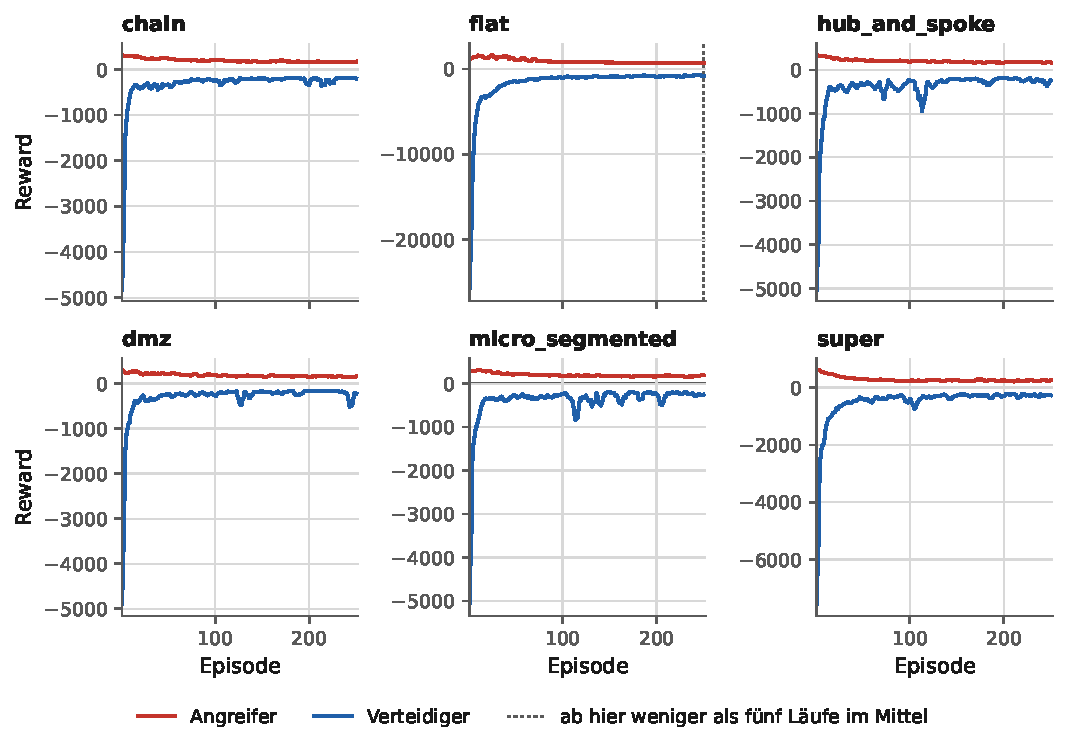
\includegraphics[width=\textwidth]{lernkurven_flat}
  \caption[Lernkurven auf \emph{flat}]{Verteidiger auf \emph{flat} gegen alle
  sechs Angreifer, gemittelt über fünf Seeds und geglättet über das gleitende
  Mittel von fünf Episoden.}
  \label{fig:lk-flat}
\end{figure}

Die Zeile \emph{flat} in \Cref{tab:reward-atk-verlauf} zeigt den Angreifer in fünf
der sechs Spalten auf einem höheren Endniveau als in jeder anderen
verteidigten Topologie; einzig der DMZ-Angreifer endet auf seiner
Heimattopologie mit 150 knapp über den 147. In \Cref{fig:lk-flat} kommt
entsprechend keine der sechs Verteidigerkurven der Nulllinie nennenswert
nahe. Am deutlichsten ist das im Teilbild des eigenen Angreifers, oben in der
Mitte; \Cref{tab:reward-ende} beziffert es: Startniveau $-8381$, Endniveau
$-710$, während dieselbe Topologie gegen alle übrigen Angreifer zwischen
$-168$ und $-197$ endet.

\begin{figure}[H]
  \centering
  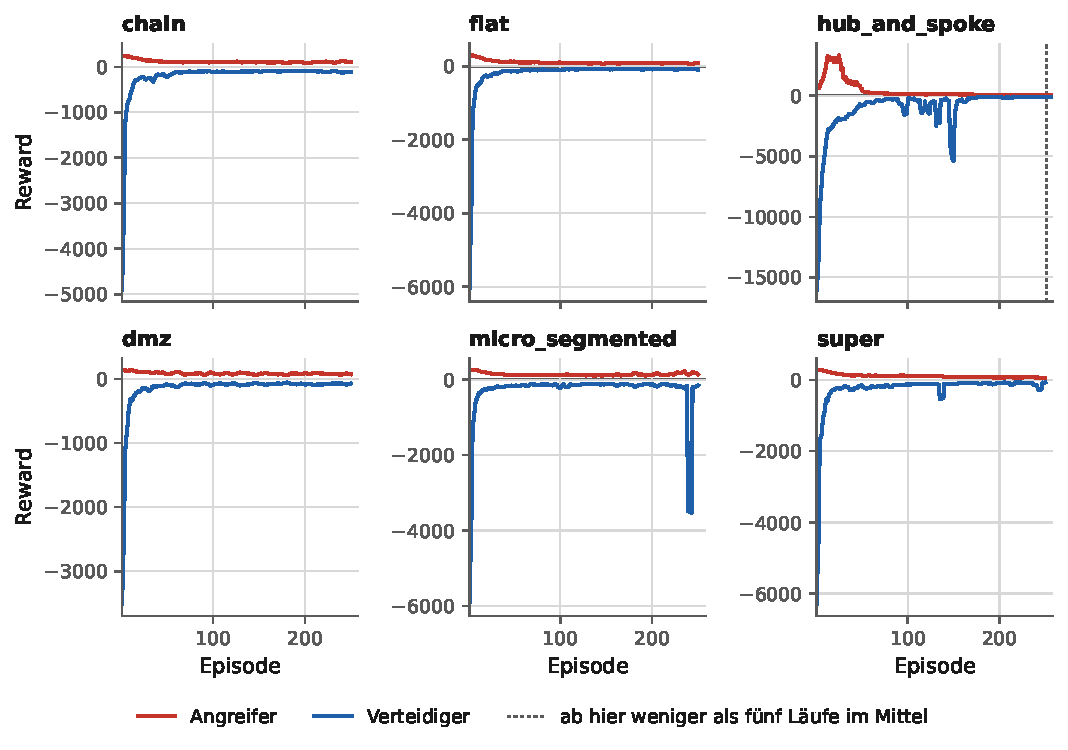
\includegraphics[width=\textwidth]{lernkurven_hub_and_spoke}
  \caption[Lernkurven auf \emph{hub\_and\_spoke}]{Verteidiger auf
  \emph{hub\_and\_spoke} gegen alle sechs Angreifer.}
  \label{fig:lk-hs}
\end{figure}

In \emph{hub\_and\_spoke} (\Cref{fig:lk-hs}) fällt das Teilbild des eigenen
Angreifers durch etwas anderes auf. Dort steigt die Mittelkurve des Angreifers
zunächst bis auf über $+3300$ in Episode~25, also weit über das Niveau aller
übrigen Teilbilder, und fällt dann über das Training fast vollständig wieder ab. Der Verteidiger beginnt im Startniveau bei
$-7910$ und endet bei $-78$ (\Cref{tab:reward-ende}). Der Anfang ist dabei kein
Spiegelbild: Der Verteidiger verliert ein Vielfaches dessen, was der Angreifer
gewinnt, weil zur Kopplung noch die \ac{SLA}-Strafe hinzukommt. Erst am Ende
stehen die beiden Werte einander spiegelbildlich gegenüber, und genau das
zeigt an, dass keine Brüche mehr anfallen. Der auf dieser Topologie trainierte
Angreifer beginnt also mit Abstand am stärksten und verliert im Verlauf
90~Prozent seines Rewards. Am Ende ist er von den übrigen fünf Angreifern
dieser Zeile nicht mehr zu unterscheiden, die zwischen 62 und 110 liegen
(\Cref{tab:reward-atk-verlauf}).

In dieser Abbildung fallen zudem die tiefen Einbrüche auf, etwa gegen
Episode~150 im selben Teilbild und gegen Episode~240 gegen den
Micro-Segmentation-Angreifer. Beide gehen auf einzelne Seeds zurück und haben
einen unterschiedlichen Umfang. Der erste ist eine Phase: In zwei der fünf
Läufe häufen sich zwischen Episode~110 und 165 die \ac{SLA}-Brüche, in einem
über 21 und im anderen über 16 Episoden. Der zweite ist eine einzige Episode,
in der die Verfügbarkeit über \num{1668} der rund 2000 Schritte unter der
Schwelle lag.

\begin{figure}[H]
  \centering
  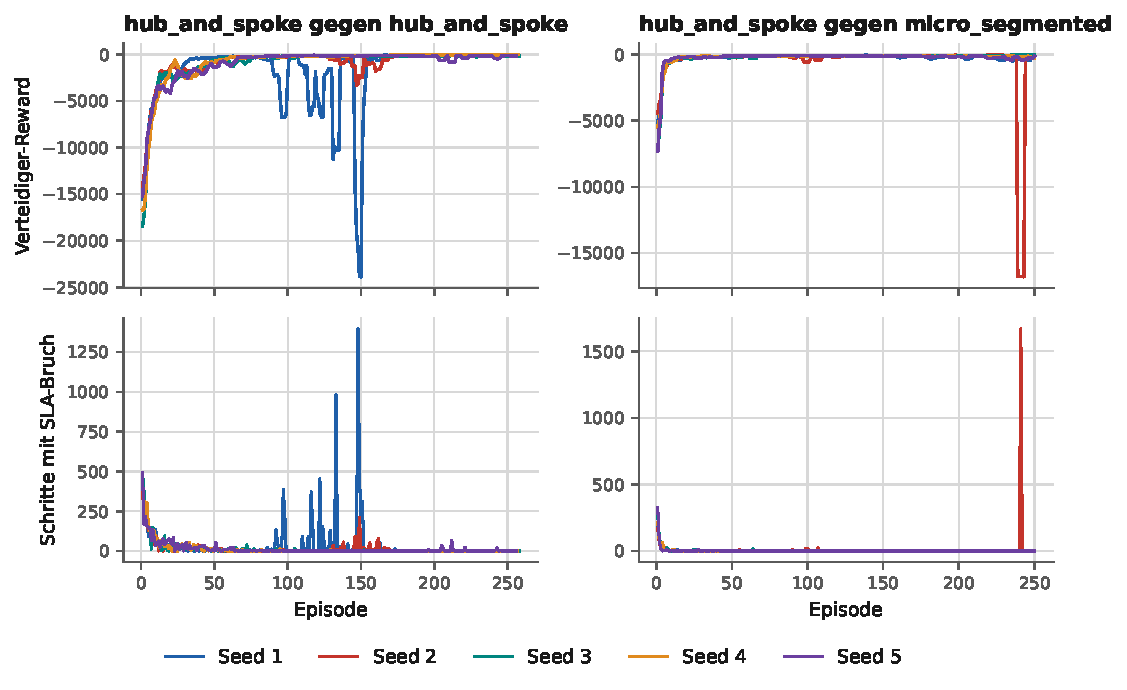
\includegraphics[width=\textwidth]{sla_einbrueche}
  \caption[Reward und \acs{SLA}-Brüche je Seed]{Verteidiger-Reward und Schritte
  mit \ac{SLA}-Bruch für die beiden auffälligen Matchups, je Seed einzeln
  aufgetragen und nicht gemittelt. Der Reward ist über fünf Episoden geglättet,
  die Bruchschritte sind es nicht.}
  \label{fig:sla-einbrueche}
\end{figure}

\Cref{fig:sla-einbrueche} stellt beides nebeneinander. Die Ausschläge der
Reward-Kurve und die Spitzen der Bruchschritte liegen an denselben Episoden,
und sie beschränken sich auf wenige Läufe: links auf zwei, von denen einer
deutlich stärker ausschlägt, rechts auf einen einzigen. Kurze Brüche
treten auch in den übrigen Seeds vereinzelt auf; Episoden mit mehreren hundert
Bruchschritten bleiben jedoch auf diese wenigen Läufe beschränkt. Im gesamten
Training gibt es nur zwölf Episoden mit mehr als 500 Bruchschritten, und acht
davon liegen in den ersten beiden Episoden ihres Laufs.

Eine Erklärung liefert der Vergleich innerhalb des Laufs mit der schwersten
Episode, also des einen betroffenen Seeds gegen den
Micro-Segmentation-Angreifer; als ruhig gelten dabei seine bruchfreien
Episoden ab Episode~51, nach der Anfangsphase.
In der Episode mit \num{1668} Bruchschritten bleibt die Zahl
der Reimages mit 117 gegenüber 112 im Median praktisch unverändert. Die Zahl
der Sperren steigt dagegen von 7 auf 36, und keine einzige von ihnen wird
wieder aufgehoben, gegenüber im Median 61 Freigaben in einer ruhigen Episode. Nicht das
Neuaufsetzen bricht also die Verfügbarkeit, sondern Sperren, die über den
größten Teil der Episode Bestand haben; eine gesetzte Sperre wirkt bis zu
ihrer Aufhebung fort. Eine erreichte
Policy ist demnach nicht dauerhaft stabil, und das Konvergenzkriterium aus
\Cref{sec:konvergenz} erfasst solche späten Rückfälle nicht.

Woher der Umschwung in der Policy rührt, lässt sich aus den erhobenen Daten
nicht eindeutig bestimmen. Zweierlei ist dazu festzuhalten. Erstens ist es kein
allgemeines Verhalten des Verfahrens, sondern eines einzelner Läufe: Von fünf
Seeds sind jeweils einer oder zwei betroffen, die übrigen zeigen keine solchen
Ausschläge in der Zahl der Bruchschritte.
Genau diese Streuung zwischen sonst gleichen Läufen beschreiben Henderson
et~al.\ als eigenständige Schwierigkeit von Policy-Gradient-Verfahren; sie
zeigen, dass allein die Wahl des Zufallsstartwerts zu deutlich verschiedenen
Ergebnisverteilungen führen kann und ein Mittel über wenige Läufe deshalb
keine belastbaren Schlüsse
erlaubt~\cite{henderson2019deepreinforcementlearningmatters}. Für die vorliegende Arbeit begrenzt das lediglich die Deutung: Die
Einbrüche in den Mittelkurven sind keine Aussage über die Topologie,
sondern die sichtbare Spur einzelner Seeds.

Zweitens ist der naheliegende Verdacht, eine einzelne Ausreißerepisode habe
die Policy unmittelbar verschoben, mit dem Verfahren nicht vereinbar. Genau
das verhindert die Begrenzung aus \Cref{eq:ppo-clip}: Sie deckelt, wie weit
sich die Policy je Aktualisierung von der bisherigen entfernen darf,
unabhängig davon, wie groß der Vorteil ausfällt.

Diese Grenze gilt allerdings nur für die Policy selbst. Der Critic darf
seine Prognose nach einer solchen Episode beliebig stark anpassen, und da
sich beide in der eingesetzten Umsetzung die vorderen Schichten des Netzes
teilen, wirkt seine Korrektur mittelbar auch auf den Actor -- an dessen
eigener Begrenzung vorbei. Derselbe Mechanismus trägt die rasche Rückkehr:
Sobald die Episoden wieder normal ausfallen, fallen die Schätzungen des
Critic deutlich negativer aus als das tatsächliche Geschehen. Jede
gewöhnliche Episode erscheint dadurch besser als erwartet, das zuletzt
gezeigte Verhalten wird verstärkt, und die Policy findet auf das alte
Niveau zurück. Was den Ausschlag überhaupt auslöst, erklären diese Überlegungen
nicht.

\begin{figure}[H]
  \centering
  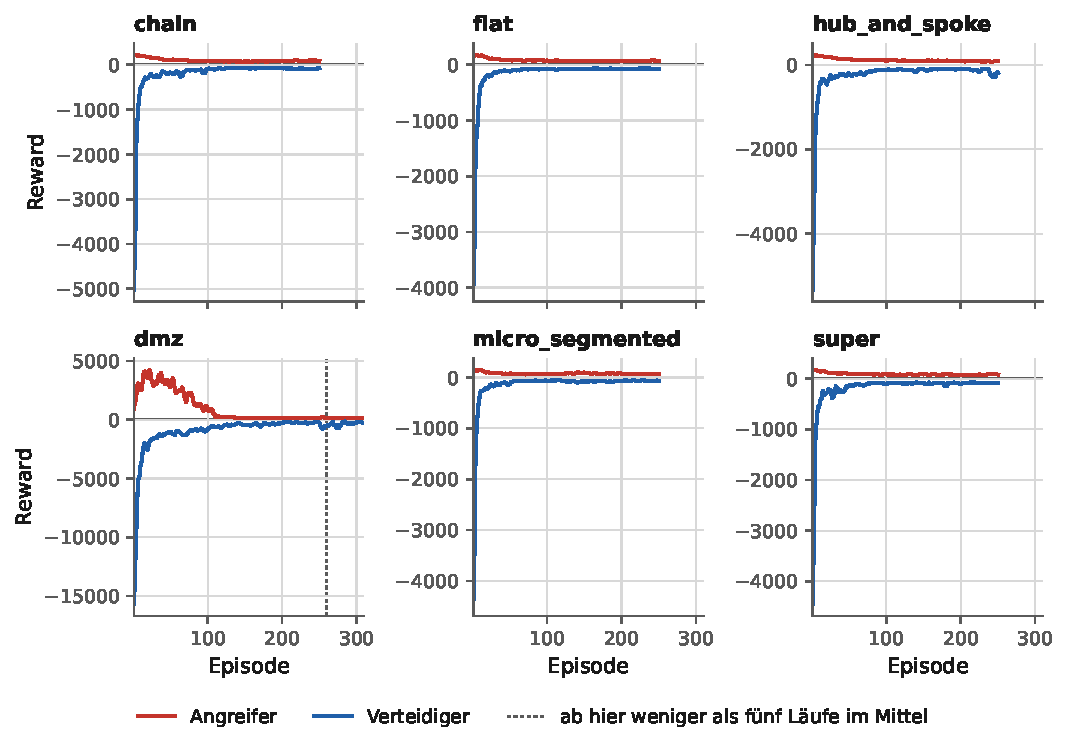
\includegraphics[width=\textwidth]{lernkurven_dmz}
  \caption[Lernkurven auf \emph{dmz}]{Verteidiger auf \emph{dmz} gegen alle
  sechs Angreifer.}
  \label{fig:lk-dmz}
\end{figure}

\emph{dmz} (\Cref{fig:lk-dmz}) zeigt dasselbe Muster, aber deutlich langsamer.
Die Mittelkurve des Angreifers steigt zunächst noch, bis auf 4257 in
Episode~22, und geht erst danach zurück: auf 2277 in Episode~75, 946 in
Episode~100 und 282 in Episode~110; von dort an ändert sich wenig mehr. Die
Mittelkurve des Verteidigers verbessert sich über denselben Zeitraum stetig
und liegt in Episode~50 bereits bei $-1030$. Da der Angreifer
eingefroren ist, lernt er selbst nichts dazu; eine gerichtete Veränderung
seiner Kurve geht deshalb auf den Verteidiger zurück, während kurzfristige
Schwankungen der Streuung zwischen den Läufen zuzuschreiben sind.
Erst nach rund 25 Episoden beginnt dieser, ihn tatsächlich zu
bremsen, und dafür braucht er dann etwa 80 weitere. In demselben
Zeitraum bricht auch die Crown-Jewel-Quote dieses Matchups ein
(\Cref{fig:cj-verlauf-dmz}); beide Größen bewegen sich also gemeinsam.

\begin{figure}[H]
  \centering
  
\includegraphics[width=\textwidth]{cj_verlauf_dmz}
  \caption[Reward und Crown-Jewel-Quote in \emph{dmz}]{Angreifer-Reward und
  Crown-Jewel-Quote im Matchup \emph{dmz} gegen \emph{dmz}.}
  \label{fig:cj-verlauf-dmz}
\end{figure}

Bis Episode~55 fällt das Crown Jewel in jeder einzelnen Episode. Danach
sinkt die Quote parallel zum Reward, auf 85~Prozent in Episode~100 und auf
ihren Tiefstwert von 26~Prozent in Episode~145. Der Rückgang des Rewards
ist also kein bloßer Punktverlust, sondern bedeutet, dass der Verteidiger
den Angreifer in einem wachsenden Teil der Episoden vom wertvollsten
System fernhält.

Danach pendelt die Quote zwischen 26 und 62~Prozent, ohne weiter zu
fallen; die noch höheren Werte am rechten Rand beruhen bereits auf weniger
als fünf Läufen. Das ist jedoch keine gemeinsame Bewegung aller Läufe,
sondern deren Streuung: Über die Episoden~150 bis 250 erreichen die fünf
Seeds Quoten von 26, 31, 37, 59 und 70~Prozent, jeder für sich weitgehend
stabil. Die gemittelte Kurve bildet damit eine Mischung aus fünf
verschiedenen, aber jeweils gefestigten Policies ab, nicht einen
Rückfall. Die Evaluation bestätigt das Niveau später mit 36~Prozent
(\Cref{tab:cj-eval}).

\begin{figure}[H]
  \centering
  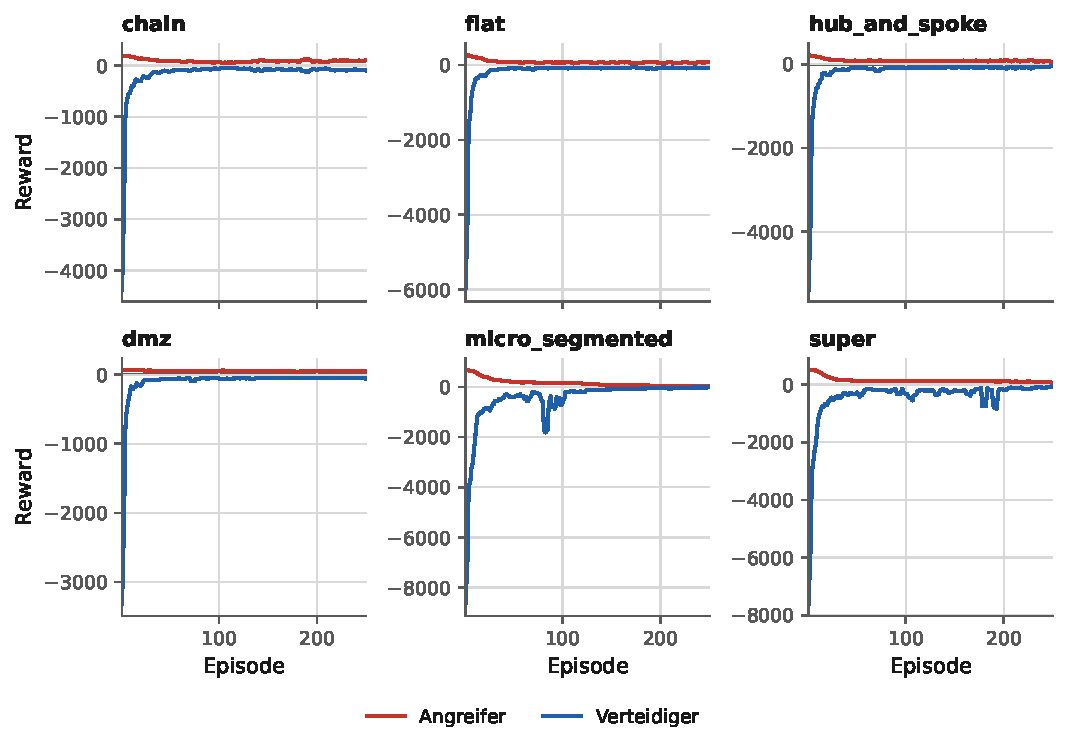
\includegraphics[width=\textwidth]{lernkurven_micro_segmented}
  \caption[Lernkurven auf \emph{micro\_segmented}]{Verteidiger auf
  \emph{micro\_segmented} gegen alle sechs Angreifer.}
  \label{fig:lk-ms}
\end{figure}

In \emph{micro\_segmented} (\Cref{fig:lk-ms}) verlaufen beide Kurven im Teilbild
des eigenen Angreifers über das gesamte Training aufeinander zu und enden bei den Niveaus $+20$
und $-20$. Anders als in \emph{dmz} beginnt der Rückgang
sofort: Die Mittelkurve fällt auf 363 in Episode~25 und 193 in Episode~50,
danach langsamer weiter. Von den vier Matchups auf der Diagonalen ist dies das einzige, in dem der
Angreifer am Ende praktisch nichts mehr erwirtschaftet. Innerhalb der
Abbildung ähnelt dem Teilbild des eigenen Angreifers einzig das des
Super-Angreifers: Dessen Mittelkurve liegt in Episode~25 mit
208 noch weit über den vier übrigen Teilbildern, die dort 58 bis 127 zeigen,
und die Verteidigerkurve beginnt gegen ihn tiefer und holt langsamer auf --
in Episode~25 steht sie bei $-494$, in den vier übrigen Teilbildern zwischen
$-72$ und $-228$. Das fügt sich in das Bild, denn der Super-Angreifer ist
der einzige weitere, der diese Topologie im Training gesehen hat, als letzte Station seines gestuften Trainings;
\Cref{sec:angreiferherkunft} nimmt das wieder auf.
Die Anfangswerte fallen zugleich am mildesten aus: Das tiefste Startniveau
liegt hier bei $-3711$ gegenüber $-8381$ in \emph{flat}
(\Cref{tab:reward-ende}). Das passt zu den nur 145 erreichbaren Punkten dieser Topologie.

Über alle vier Abbildungen hinweg zeigt sich damit dasselbe Muster: Das Teilbild
des eigenen Angreifers ist stets dasjenige mit dem tiefsten Startwert und dem
längsten Weg. Ein Verteidiger tut sich gegen den Gegner am schwersten, der
seine eigene Struktur kennt. \Cref{sec:angreiferherkunft} geht dem nach.

\Cref{tab:reward-ende} stellt Start- und Endniveau des Verteidigers
gegenüber. Am Start trägt die Diagonale in jeder Zeile mit Abstand den
tiefsten Wert; bemerkenswert ist, dass ihre Werte am Ende nicht mehr
herausstechen:
In \emph{micro\_segmented} ist sie sogar der beste Wert der Zeile, in
\emph{hub\_and\_spoke} liegt sie im Mittelfeld. Der anfängliche Rückstand gegen den
passgenauen Angreifer ist bis zum Trainingsende also aufgeholt. Die Ausnahme
ist erneut \emph{flat} gegen \emph{flat} mit $-710$, dem mit Abstand schlechtesten Wert der
Tabelle; alle übrigen 23 Zellen liegen zwischen $-20$ und $-224$. Der
zweitschlechteste Wert, $-224$ gegen den Hub-and-Spoke-Angreifer in \emph{dmz}, wird
dabei von einem einzelnen Seed bei $-839$ getragen; die übrigen vier Läufe
dieser Zelle enden zwischen $-58$ und $-86$.

\begin{table}[H]
  \centering
  \caption[Verteidiger-Reward als Start- und Endniveau]{Start- und Endniveau
  des Verteidiger-Rewards. Werte näher an null sind besser.}
  \label{tab:reward-ende}
  \footnotesize
  \setlength{\tabcolsep}{4pt}
  \begin{adjustbox}{max width=\textwidth}
  \begin{tabular}{l*{6}{r}}
    \toprule
    Verteidigt & Chain & Flat & H\,\&\,S & DMZ & Micro & Super \\
    \midrule
    Flat        & $-1118\to-182$ & \diag{$-8381\to-710$} & $-1694\to-193$ & $-1209\to-168$ & $-1318\to-188$ & $-2349\to-197$ \\
    Hub \& Spoke& $-983\to-109$ & $-951\to-64$ & \diag{$-7910\to-78$} & $-789\to-81$ & $-946\to-117$ & $-1600\to-72$ \\
    DMZ         & $-1159\to-77$ & $-977\to-67$ & $-1193\to-224$ & \diag{$-7265\to-157$} & $-978\to-62$ & $-866\to-76$ \\
    Micro-Seg.  & $-735\to-76$ & $-1156\to-74$ & $-904\to-49$ & $-434\to-53$ & \diag{$-3711\to-20$} & $-2799\to-83$ \\
    \bottomrule
  \end{tabular}
  \end{adjustbox}
\end{table}

Diese Zahlen sind allerdings nur innerhalb einer Zeile vergleichbar, nicht
zwischen den Zeilen. Der Verteidiger-Reward ist über die Grundkopplung an den
des Angreifers gebunden, und der erreichbare Punktevorrat unterscheidet sich
je Topologie: In \emph{micro\_segmented} sind vom Einstiegsknoten aus nur 145
der 235 Punkte überhaupt erreichbar (\Cref{sec:topomodell}). Ein Teil des
besseren Rewards geht dort also allein darauf zurück, dass weniger zu holen
war; welcher Anteil das ist, lässt sich der Zahl nicht entnehmen. Die Aussagen zur
Wirksamkeit stützen sich deshalb in \Cref{sec:wirksamkeitergebnis} auf
Größen, die von der Reward-Skala unabhängig sind.

\section{Crown-Jewel-Quote im Trainingsverlauf}
\label{sec:cj-verlauf}

Die Reward-Kurven laufen in allen 24 Matchups früh auf ein Niveau zu, auf dem
sie anschließend verharren. Daraus ließe sich schließen, dass auch die
Verteidigung ab diesem Punkt nicht mehr besser wird. Die Crown-Jewel-Quote
widerspricht dem. Sie ist zugleich die Größe, an der die Fragestellung
unmittelbar hängt, denn sie sagt, ob der Angreifer das wertvollste System
erreicht.

\begin{figure}[H]
  \centering
  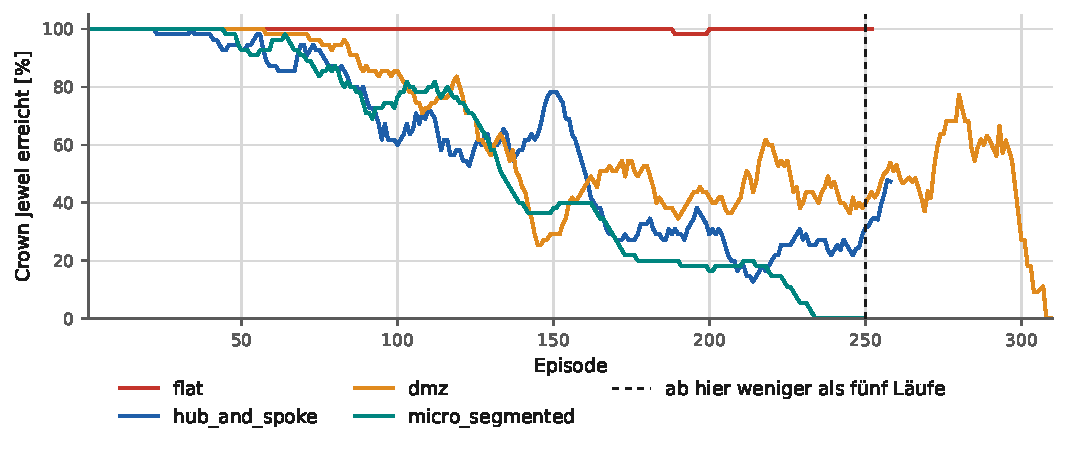
\includegraphics[width=\textwidth]{cj_verlauf_diagonale}
  \caption[Crown-Jewel-Quote im Trainingsverlauf]{Anteil der Episoden mit
  erreichtem Crown Jewel für die vier Matchups auf der Diagonalen. Die Quote
  ist über ein Fenster von elf Episoden und alle fünf Seeds gebildet, also über
  55~Episoden je Punkt.}
  \label{fig:cj-diagonale}
\end{figure}

\Cref{fig:cj-diagonale} trennt die vier Topologien deutlicher als jede andere
Größe dieses Kapitels. Zu Beginn erreicht der Angreifer das Ziel überall in
jeder Episode. Danach gehen die Verläufe auseinander:

\begin{itemize}
  \item In \emph{flat} verhindert der Verteidiger über das gesamte Training
    keinen einzigen Zugriff auf das Crown Jewel, von einer einzigen Episode
    abgesehen.
  \item In \emph{micro\_segmented} fällt sie stetig und liegt kurz nach
    Episode~230 bei null; über die letzten zwanzig Episoden aller fünf
    Seeds erreicht der Angreifer das Ziel in keiner einzigen.
  \item \emph{hub\_and\_spoke} und \emph{dmz} liegen dazwischen und kommen auf
    28 beziehungsweise 42~Prozent in den letzten zwanzig Episoden.
\end{itemize}

Bemerkenswert ist der Zeitpunkt. In \emph{micro\_segmented} sinkt die Quote
zwischen Episode~150 und 230 von 38 auf 5~Prozent, während der Reward in
diesem Abschnitt nur noch von etwa $-100$ auf $-20$ steigt. Am Reward gemessen
geschieht dort fast nichts mehr, an der Crown-Jewel-Quote gemessen das
Entscheidende. 
Der Grund liegt in der Reward-Konstruktion: Ein Zugriff, der
verhindert wird, schlägt sich nur mit dem Wert des Zielknotens von
100~Punkten nieder, weil dem Angreifer nichts genommen, sondern nur nichts
gegeben wird (\Cref{sec:marlon-original}).

In \emph{dmz} erreicht der Angreifer das Crown Jewel auch nach dem
Einpendeln regelmäßig, ohne dass sich das im Reward niederschlägt
(\Cref{fig:cj-verlauf-dmz}, bei den Lernkurven). Der Grund liegt in der
Kopplung aus Verlust und Rückeroberung (\Cref{sec:rewards}). Über die
Episoden~150 bis 250 verliert der Angreifer in den Episoden mit
erreichtem Crown Jewel im Median 2035~Punkte durch neu aufgesetzte Knoten,
gegenüber 1552 in den übrigen. Er nimmt das Ziel also,
verliert es wieder und nimmt es erneut, und jede dieser Runden gleicht sich
aus. Am Ende trennt die Episoden mit erreichtem Crown
Jewel von denen ohne ein Unterschied von 175 zu 126~Punkten -- weniger als
die 100~Punkte, die das gehaltene Crown Jewel allein wert wäre.

Beide Größen messen demnach Verschiedenes: Die Crown-Jewel-Quote sagt, ob der
Angreifer das Ziel überhaupt erreicht, der Reward, ob er es halten kann.
Sie bewegen sich dennoch in dieselbe Richtung. Ordnet man die fünf Seeds nach ihrer Quote, so
steigt der Reward-Median mit ihr, von 123 bei 26~Prozent bis 188 bei
70~Prozent. Erst aus beiden zusammen ergibt sich ein Bild, wie in
\Cref{sec:metriken} angelegt.

\section{Gehaltene Knoten im Trainingsverlauf}
\label{sec:knoten-verlauf}

Ob das Crown Jewel gefallen ist, beantwortet noch nicht, wie weit der Angreifer
insgesamt vorgedrungen ist. Ein Netz, in dem er acht Knoten hält, und eines, in
dem er auf dem Einstiegsknoten festsitzt, stehen in dieser Quote gleich, sofern
das Ziel in beiden Fällen unangetastet blieb. Dafür dient die dritte Zielgröße
aus \Cref{sec:metriken}, die größte Zahl gleichzeitig kompromittierter Knoten
je Episode. Der Einstiegsknoten zählt dabei mit: Ein Wert von 1,0 bedeutet, dass
der Angreifer über ihn nicht hinausgekommen ist.

\begin{figure}[H]
  \centering
  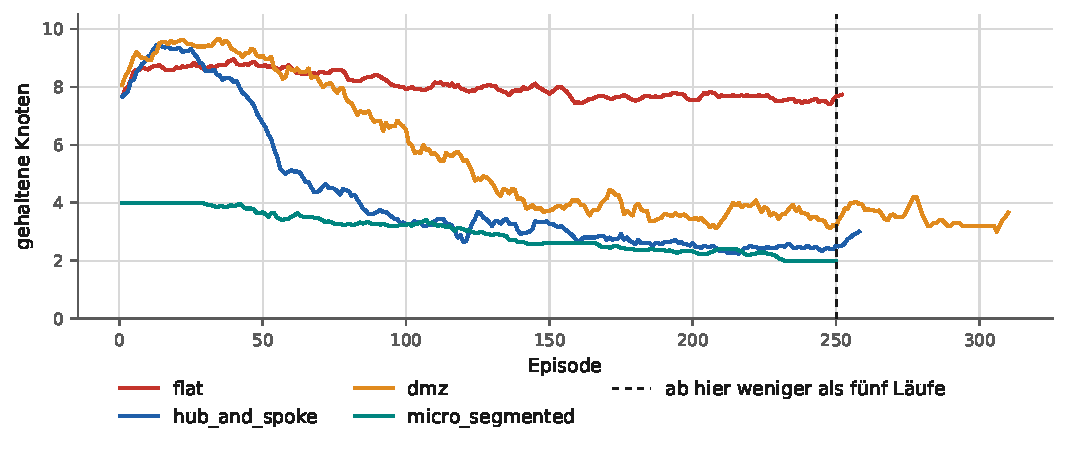
\includegraphics[width=\textwidth]{knoten_verlauf_diagonale}
  \caption[Gehaltene Knoten im Trainingsverlauf]{Größte Zahl gleichzeitig
  gehaltener Knoten je Episode für die vier Matchups auf der Diagonalen,
  gemittelt über fünf Seeds und geglättet über fünf Episoden. Von zehn Knoten
  im Netz.}
  \label{fig:knoten-diagonale}
\end{figure}

In \emph{dmz} und \emph{hub\_and\_spoke} steigt die Mittelkurve zunächst noch
an und erreicht 9,6 beziehungsweise 9,4. Der Angreifer hält dort in den meisten
Episoden das gesamte Netz. Erst danach setzt der Rückgang ein.
\emph{micro\_segmented} beginnt dagegen bei 4,0 und hält damit ebenfalls
alles, was von dort aus überhaupt erreichbar ist (\Cref{sec:topomodell}).

Die Abbildung zeigt nur die Diagonale, alle 24 Matchups zeigt
\Cref{app:knoten}. Zieht man sie alle heran, so
liegen 21 von ihnen am Ende des Trainings zwischen 1,8 und 2,5. Der
Verteidiger drückt den Angreifer also im Regelfall auf ein bis zwei eroberte
Rechner zurück. Drei Zellen weichen davon ab, und zwei davon sind in der
Abbildung zu sehen: \emph{dmz} gegen \emph{dmz} mit 3,4 und \emph{flat}
gegen \emph{flat} mit 7,5, dazu \emph{flat} gegen den Super-Angreifer mit
3,0.

Auffällig ist davon nur \emph{flat} gegen \emph{flat}: Auch dort hält der
Angreifer anfangs fast das gesamte Netz, doch anders als in \emph{dmz} und
\emph{hub\_and\_spoke} setzt der Rückgang nie ein -- die Kurve bleibt über
das gesamte Training nahe ihrem Höchstwert, der Angreifer behält dauerhaft
rund drei Viertel des Netzes.

\section{Konvergenz}
\label{sec:konvergenzergebnis}

Das in \Cref{sec:konvergenz} beschriebene Kriterium wird von allen 120 Läufen
erfüllt, im Median in Episode~42. Der früheste überhaupt mögliche Wert ist
Episode~39, der früheste gemessene Episode~40. Die Mediane je verteidigter Topologie
liegen zwischen 41 und 42,5 und unterscheiden sich damit nicht sonderlich
voneinander.
Sämtliche Läufe gelten also nahezu unmittelbar an der unteren Grenze des
Kriteriums als konvergiert, obwohl sie bis zur Episode~250 laufen.

Dieser Befund ist kein Ergebnis über Topologien, sondern eines über das
Kriterium. Es misst die Restunruhe der letzten Episoden im Verhältnis zur
bisherigen Reward-Spanne des Laufs. Genau diese Spanne wird durch die ersten Episoden sehr groß, die je nach
Lauf im fünfstelligen Bereich liegen, und jede spätere
Verbesserung wirkt daran gemessen klein. Ein Lauf gilt deshalb bereits als
ruhig, während er sich tatsächlich noch verbessert.

\emph{dmz} gegen \emph{dmz} zeigt das exemplarisch: Die Spanne wird von der ersten
Episode bestimmt, die je nach Seed zwischen rund $-15\,000$ und
$-31\,000$ liegt; fünf Prozent davon sind 750 bis 1550 Punkte. Zu dem Zeitpunkt, an dem das Kriterium zutrifft, im Median in
Episode~49, steht die Mittelkurve erst
bei rund $-1000$; bis zum Trainingsende verbessert sich der Reward weiter,
auf Endniveaus zwischen $-133$ und $-196$ je Seed. Diese Verbesserung
verteilt sich über zweihundert Episoden und bleibt damit je
Fenster unter der Schwelle. Das Kriterium trennt das Ende der Unruhe nicht vom Ende
der Verbesserung.

Eine Spur des in \Cref{sec:lernkurven} beschriebenen Musters bleibt dennoch
erkennbar. In drei der vier Zeilen trägt die Diagonale den höchsten Wert, in
\emph{micro\_segmented} teilt sie ihn mit der Zelle gegen den
Super-Angreifer: \emph{dmz} gegen \emph{dmz} konvergiert im Median erst in
Episode~49, \emph{hub\_and\_spoke} gegen sich selbst in 47, \emph{micro\_segmented} in 46 und
\emph{flat} in 44, gegenüber 40
bis 46 in allen übrigen Zellen (\Cref{tab:konvergenz-vergleich}, jeweils
der Wert vor dem Schrägstrich). Die Richtung stimmt
also mit den übrigen Größen überein, die Spreizung ist aber so gering, dass
sich darauf keine Aussage stützen lässt.

Dass die Topologien sich nicht trennen, könnte an der Wahl der Schwelle liegen.
Das Kriterium besteht aus zwei voneinander unabhängigen Bedingungen, die
Verschiedenes messen: Die Streuung erfasst das Rauschen der Kurve, der Trend
erfasst, ob die Verbesserung aufgehört hat. Beide erhalten in
\Cref{sec:konvergenz} denselben Wert von 0,05 der Spanne, was eine Konvention
ist und keine Notwendigkeit.

Nachgerechnet zeigt sich, dass davon nur eine der beiden Bedingungen wirksam
ist. Die Streuung ist in fast allen 120 Läufen von dem Moment an erfüllt, ab
dem das Kriterium überhaupt geprüft wird; scheitert eine Prüfung vor der
Konvergenz, dann in aller Regel am Trend. Was den Zeitpunkt bestimmt, ist also
allein der Trendtest, und dessen Toleranz von 5~Prozent der Gesamtspanne ist weit
gefasst.

Als Gegenprobe wurde die Schwelle des Trends deshalb auf 0,01 gesenkt, die der
Streuung blieb bei 0,05. Am Kriterium selbst ändert das nichts, nur an einer
seiner beiden Zahlen.

\begin{table}[H]
  \centering
  \caption[Konvergenzepisoden je Matchup]{Konvergenzepisode je Matchup als
  Median der fünf einzeln geprüften Seeds; vor dem Schrägstrich beim
  Trendtest mit Schwelle 0,05, dahinter mit 0,01. Hervorgehoben ist die
  Diagonale.}
  \label{tab:konvergenz-vergleich}
  \footnotesize
  \setlength{\tabcolsep}{4pt}
  \begin{tabular}{l*{6}{r}}
    \toprule
    Verteidigt & Chain & Flat & H\,\&\,S & DMZ & Micro & Super \\
    \midrule
    Flat        & 41\,/\,58 & \diag{44\,/\,72} & 43\,/\,55 & 41\,/\,59 & 43\,/\,58 & 42\,/\,76 \\
    Hub \& Spoke& 41\,/\,50 & 41\,/\,55 & \diag{47\,/\,88} & 40\,/\,51 & 41\,/\,50 & 44\,/\,53 \\
    DMZ         & 41\,/\,49 & 42\,/\,53 & 41\,/\,59 & \diag{49\,/\,95} & 41\,/\,59 & 42\,/\,68 \\
    Micro-Seg.  & 40\,/\,57 & 42\,/\,49 & 41\,/\,50 & 40\,/\,52 & \diag{46\,/\,66} & 46\,/\,60 \\
    \bottomrule
  \end{tabular}
\end{table}

Auch mit dem strengeren Trendtest erfüllen alle 120 Läufe das Kriterium; der
Median wandert von Episode~42 auf 58,5. Die Topologien trennen sich weiterhin
nicht: Ihre Mediane liegen zwischen 53 und 62, die Quartile der 30 Läufe je
Topologie reichen von 55 bis 77 in \emph{flat} und von 50 bis 62 in
\emph{micro\_segmented} und überlappen damit fast vollständig.

Sichtbar wird dagegen etwas anderes. Betrachtet man nicht die Zeilen
gegeneinander, sondern die Zellen innerhalb einer Zeile, so tritt die
Diagonale hervor (\Cref{tab:konvergenz-vergleich}, Werte nach dem
Schrägstrich). Ihre Mediane liegen zwischen Episode~66 und 95, die der übrigen
20~Zellen zwischen 49 und 76. In drei der vier Zeilen ist die Diagonale die Zelle mit der spätesten
Konvergenz, in \emph{flat} die zweitspäteste hinter der Zelle gegen den
Super-Angreifer. Beim Kriterium aus \Cref{sec:konvergenz} war dieser
Unterschied kaum erkennbar. Der Befund fügt sich damit in die übrigen Größen
ein, die in \Cref{sec:angreiferherkunft} zusammengeführt werden.

Angegeben ist hier der Median der fünf Seeds einer Zelle, nicht ihr Mittel.
Einzelne Läufe konvergieren sehr viel später als die übrigen vier ihrer Zelle,
etwa \emph{flat} gegen den Hub-and-Spoke-Angreifer mit 48, 49, 55, 63 und 164.
Das Mittel dieser Zelle läge bei 76 und damit über der Diagonalen, obwohl vier
ihrer fünf Läufe zu den schnellsten der Zeile gehören.

Für die Frage nach der Topologie bleibt es beim Ergebnis: Bei fünf Seeds je
Zelle ist ein Einfluss auf die Lerngeschwindigkeit nicht nachweisbar.
Ausgeschlossen ist er damit nicht, die Daten tragen den Nachweis nur nicht.

Als Maß der Lerneffizienz ist der Konvergenzzeitpunkt in dieser Form deshalb
nur eingeschränkt geeignet. Dass die Läufe ihr volles Schrittbudget erhielten
und nicht beim Erfüllen des Kriteriums abgebrochen wurden
(\Cref{sec:konvergenz}), erweist sich hier als nützlich: Beide Varianten ließen
sich nachträglich auf vollständige Kurven anwenden, und der Vergleich in
\Cref{tab:konvergenz-vergleich} wurde dadurch überhaupt erst möglich. Wäre wie
im Referenzlauf abgebrochen worden, stünde am Ende eine einzelne Zahl, deren
Zustandekommen sich nicht mehr prüfen ließe.

Der Vergleich der Topologien stützt sich in dieser Arbeit deshalb auf das
erreichte Niveau (\Cref{sec:lernkurven} bis \Cref{sec:knoten-verlauf}) und auf
die Wirksamkeit der fertig trainierten Policy
(\Cref{sec:wirksamkeitergebnis}). \Cref{sec:limitationen} schlägt ein Maß vor,
das ohne die Normierung auf die Gesamtspanne auskommt.

\section{Aktionsverhalten des Verteidigers}
\label{sec:aktionen}

Über alle 120 Läufe gemittelt sinkt der Anteil der Sperren von 16~Prozent in
den ersten 25 Episoden auf 2~Prozent ab Episode~101. Der Verteidiger gibt das
Sperren also überwiegend auf, jedoch nicht vollständig: In
87,8~Prozent aller Episoden ist zu jedem Zeitpunkt
mindestens ein Knoten aktiv abgeschirmt. Zurück geht die Häufigkeit, mit der
Sperren umgesetzt werden, nicht ihr Bestand.

Zugleich steigt der Anteil ungültiger Aktionen von 38 auf 62~Prozent. Eine
ungültige Aktion kostet nichts und überspringt den Zug
(\Cref{sec:marlon-original}); sie ist damit der billigste Weg, nichts zu tun.
Der Aktionsraum des Verteidigers enthält keine ausdrückliche Aktion dafür.
Dasselbe gilt für Freigaben auf Knoten, die ohnehin nicht gesperrt sind: Sie
sind folgenlos. Freigaben machen über alle Läufe hinweg 36,8~Prozent aller Aktionen aus
und stehen damit nach den ungültigen Aktionen an zweiter Stelle.
Beide Anteile sind deshalb nicht als Verhalten zu lesen,
sondern zum größten Teil als Untätigkeit; einzelne Freigaben mögen berechtigt sein, aus den erhobenen Zählungen
lässt sich das jedoch nicht trennen.
Aussagekräftig bleiben Sperren und Reimages sowie ihr Verhältnis zueinander.

\Cref{fig:aktionen-verlauf} zeigt beide Aktionsarten im Verlauf. Die Bewegung
geht in allen vier Topologien in dieselbe Richtung, aber unterschiedlich weit.

\begin{figure}[H]
  \centering
  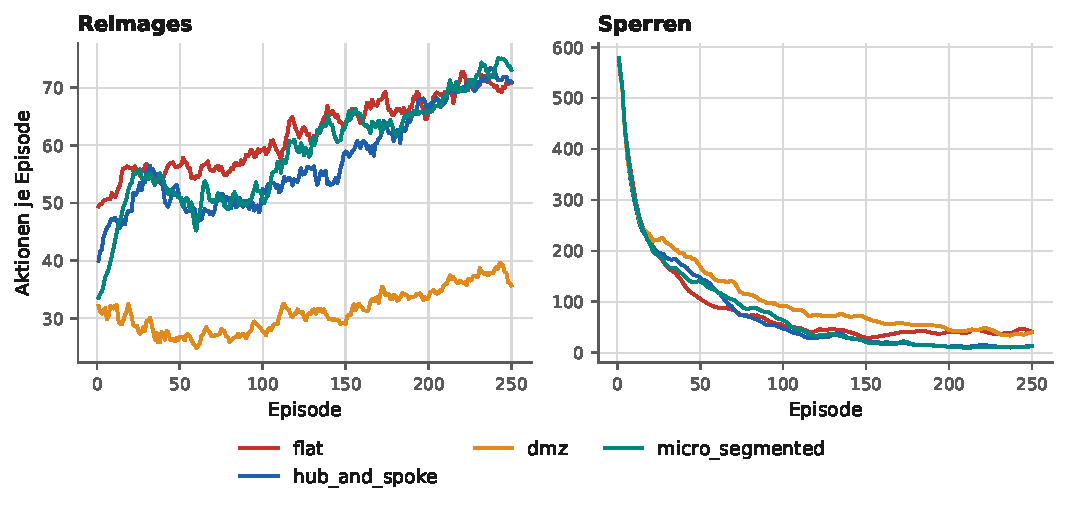
\includegraphics[width=\textwidth]{aktionen_verlauf}
  \caption[Reimages und Sperren im Trainingsverlauf]{Reimages und Sperren je
  Episode, gemittelt über die sechs Angreifer und fünf Seeds einer Topologie und
  geglättet über fünf Episoden. Die Kurven enden beim kürzesten der 30 Läufe,
  weil sich die Zusammensetzung des Mittels danach ändern würde.}
  \label{fig:aktionen-verlauf}
\end{figure}

Die Sperren gehen überall zurück, von mehreren hundert je Episode zu Beginn
auf 11 bis 45 am Ende. Der Rückgang ist aber ungleich: \emph{hub\_and\_spoke} und
\emph{micro\_segmented} landen bei 11 beziehungsweise 12, \emph{dmz} bei 37
und \emph{flat} bei 45. Umgekehrt steigen die
Reimages von 33 bis 51 auf 72 bis 75, mit \emph{dmz} als Ausnahme, dessen Zahl mit
36 bei etwa der Hälfte der übrigen liegt.

Der Verteidiger verlagert also sein Gewicht vom Sperren auf das Neuaufsetzen,
und zwar unabhängig von der Topologie. Bemerkenswert ist, dass ausgerechnet
\emph{flat} am Ende am häufigsten sperrt. Die naheliegende Deutung, der
Verteidiger gebe dort das Sperren auf, trifft also nicht zu.

Wie gut diese Sperren gesetzt sind, zeigt der Abwehrbonus
(\Cref{fig:abwehrbonus-verlauf}). Er ist so gebaut, dass eine Sperre gegen eine
bestehende Bedrohung positiv zählt und eine Sperre ohne Bedrohung negativ
(Gleichung~\ref{eq:abwehrbonus}); sein Vorzeichen zeigt damit an, ob die Sperren eines Laufs überwiegend
gegen eine bestehende Bedrohung standen.

\begin{figure}[H]
  \centering
  
\includegraphics[width=\textwidth]{abwehrbonus_verlauf}
  \caption[Abwehrbonus im Trainingsverlauf]{Abwehrbonus je Episode, gebildet
  wie in \Cref{fig:aktionen-verlauf}. Positive Werte bedeuten, dass die
  gesetzten Sperren überwiegend gegen eine bestehende Bedrohung standen.}
  \label{fig:abwehrbonus-verlauf}
\end{figure}

Alle vier Topologien beginnen deutlich im Negativen, weil ein untrainierter
Verteidiger wahllos sperrt. Der anschließende Anstieg gegen null ist für sich
genommen aber noch kein Zeichen besseren Sperrens, denn der Bonus folgt
zunächst schlicht dem Sperrvolumen aus \Cref{fig:aktionen-verlauf}: Wo kaum
noch gesperrt wird, fällt auch kaum noch Bonus an. \emph{hub\_and\_spoke}
und \emph{micro\_segmented} erreichen die Nähe der Null mit Endniveaus von $-3{,}6$
und $-0{,}3$ auf genau diesem Weg. Sie legen das Sperren fast vollständig ab,
und die wenigen verbliebenen Sperren stehen unverändert überwiegend
nicht gegen eine bestehende Bedrohung.

Anders \emph{dmz}, dessen Endniveau mit $+0{,}6$ als einziges im Positiven
liegt. Dort pendelt sich das Sperrvolumen bei rund 30 bis 40 Sperren je
Episode ein, und diese treffen zunehmend: Ab Episode~150 fällt in gut der
Hälfte der Episoden ein positiver Bonus an, gegen drei der sechs Angreifer
ist die Bilanz im Mittel sogar positiv (\Cref{app:abwehr}). Es ist zugleich die Topologie, in
der sich das Sperren auszahlt: Vergleicht man je Matchup die stärker mit
den schwächer gesperrten Episoden nach Episode~150, so steht der
Verteidiger in den stärker gesperrten im Median 13~Punkte besser da und der Angreifer 11~Punkte schlechter. Die Zonenübergänge dieser
Topologie sind Engpässe; einer Sperre dort kann der Angreifer nicht
ausweichen. Das erklärt zugleich die Ausnahmerolle beim Neuaufsetzen aus
\Cref{fig:aktionen-verlauf}: Wer den Angreifer an den Engpässen abfängt,
hat weniger neu aufzusetzen.

\emph{flat} bleibt im Endniveau bei $-14{,}2$ stehen. Mit dem Ausreißer aus
\Cref{tab:reward-ende} hat das allerdings nichts zu tun: Ausgerechnet gegen
den eigenen Angreifer sperrt der Verteidiger ab Episode~150 im Median gar
nicht mehr, sein Bonus liegt bei null (\Cref{app:abwehr}). Der Ausreißer ist schlicht die
Grundkopplung: Der eigene Angreifer erwirtschaftet am Ende 664 Punkte
(\Cref{tab:reward-atk-verlauf}), und der Verteidiger spiegelt sie. Die Belastung stammt aus den übrigen
fünf Matchups, in denen der Verteidiger das Sperren nicht ablegt, obwohl es
sich dort nach \Cref{eq:abwehrbonus} kaum lohnen kann: Jeder Knoten in
\emph{flat} hat neun Vorgänger, und weil der Angreifer in diesen Matchups
auf zwei bis drei Knoten zurückgedrängt ist, sind fast alle davon
unkompromittiert -- eine stehende Sperre zählt damit beinahe mit dem vollen
negativen Beitrag, und genau das zeigt der anhaltend negative Bonus. Anders als in \emph{dmz} zahlt sich das nicht aus: In den stärker
gesperrten Episoden steht der Verteidiger im Median 16~Punkte schlechter,
während der Angreifer kaum gebremst wird -- die Zahl seiner gehaltenen
Knoten ändert sich nicht, denn im vollvermaschten Netz weicht er einer
Sperre schlicht auf einen anderen Knoten aus. Der Hebel des
Ratenverhältnisses aus \Cref{sec:abwehrbonus} greift hier nicht, denn er
setzt voraus, dass die Sperre einen Knoten schützt, den der Angreifer
andernfalls hielte. Warum die Policy das Verhalten dennoch beibehält, lässt
sich aus den Daten nicht bestimmen; der negative Abwehrbonus von rund 18~Punkten je Episode ist
klein gegen die Streuung des Episoden-Rewards, und entsprechend schwach ist
das Signal, das er dagegen setzt. Beide Vergleiche sind zudem Beobachtungen innerhalb der gelernten
Policies, keine kontrollierten Eingriffe.

\section{Wirksamkeit der trainierten Verteidiger}
\label{sec:wirksamkeitergebnis}

In der Evaluation (\Cref{sec:evaluation}) gibt es keinen Verlauf mehr: Je Zelle wird
erst der Median über die 25 Episoden eines Seeds gebildet, dann der Median
über die fünf Seeds; Quoten fassen alle 125 Episoden einer Zelle zusammen.
Die Stufe ohne Verteidiger liefert den Bezugspunkt für den Restanteil, der
zufällige Verteidiger trennt den Beitrag des Trainings vom zufälligen Handeln.

Der Restanteil liegt für das trainierte
Modell zwischen 0,4 und 12,1~Prozent und damit in \emph{jeder} der 24 Zellen
unter dem des Zufallsverteidigers, der zwischen 5 und 37~Prozent erreicht
(\Cref{tab:restanteil}). Das Training bewirkt also
durchgängig mehr als zufälliges Handeln, und der Abstand ist deutlich: Im
Referenzlauf hatte der zufällige Verteidiger noch nahezu gleichauf mit dem
trainierten Modell gelegen (\Cref{sec:marlon-fehler}); nach dem Umbau
trennt beide in jeder Zelle ein klarer Abstand, am größten in
\emph{micro\_segmented}: Dort liegt der Restanteil des trainierten
Modells im Mittel 16,4~Prozentpunkte unter dem des
Zufallsverteidigers. Einschränkungen
dieser Schlussfolgerung behandelt \Cref{sec:limitationen}.

\begin{table}[H]
  \centering
  \caption[Restanteil in der Evaluation]{Restanteil des Angreifer-Rewards
  gegen den trainierten Verteidiger, in
  Prozent des ungeschützten Netzes; dieses selbst liegt definitionsgemäß bei
  100. In Klammern der Wert des Zufallsverteidigers. Niedriger ist besser.}
  \label{tab:restanteil}
  \small
  \begin{tabular}{l*{6}{r}}
    \toprule
    Verteidigt & Chain & Flat & H\,\&\,S & DMZ & Micro & Super \\
    \midrule
    Flat         & 8,8 (14) & 12,1 (19) & 9,0 (16) & 7,6 (12) & 8,7 (15) & 3,0 (9)  \\
    Hub \& Spoke & 5,5 (11) & 6,4 (15)  & 0,5 (10) & 3,9 (6)  & 9,8 (19) & 0,4 (5)  \\
    DMZ          & 4,1 (9)  & 3,1 (7)   & 3,8 (10) & 2,4 (10) & 4,7 (9)  & 3,6 (7)  \\
    Micro-Seg.   & 4,3 (11) & 4,9 (16)  & 3,0 (22) & 10,2 (12)& 1,2 (37) & 3,6 (27) \\
    \bottomrule
  \end{tabular}
\end{table}

Die Crown-Jewel-Quote bestätigt das Bild und schärft es
(\Cref{tab:cj-eval}). Gegen das trainierte Modell erreicht der Angreifer das Crown Jewel in
nahezu allen Zellen deutlich seltener als gegen den Zufallsverteidiger. In
\emph{micro\_segmented} fällt die Quote bei drei von sechs Angreifern auf
exakt null -- beim eigenen Angreifer, der gegen den Zufallsverteidiger noch
jede Episode gewann; der Chain- und der Flat-Angreifer kommen in je einer
einzigen der 125 Episoden einer Zelle durch.
Das andere Extrem ist erneut \emph{flat} gegen den eigenen Angreifer mit
99,2~Prozent: Hier erreicht der Angreifer das Crown Jewel praktisch in jeder
Episode, obwohl ein trainierter Verteidiger im Netz steht.

\begin{table}[H]
  \centering
  \caption[Crown-Jewel-Quote in der Evaluation]{Anteil der Episoden mit
  erreichtem Datenbankserver gegen den trainierten Verteidiger, in Prozent.
  Die kleine Zeile darunter nennt Zufallsverteidiger und ungeschütztes
  Netz.}
  \label{tab:cj-eval}
  \footnotesize
  \setlength{\tabcolsep}{4pt}
  \begin{adjustbox}{max width=\textwidth}
  \begin{tabular}{l*{6}{r}}
    \toprule
    Verteidigt & Chain & Flat & H\,\&\,S & DMZ & Micro & Super \\
    \midrule
    Flat         & 51,2 & 99,2 & 53,6 & 25,6 & 49,6 & 84,0 \\
    \multicolumn{1}{r}{\scriptsize Zufall\,/\,ohne} & \scriptsize 92\,/\,92 & \scriptsize 100\,/\,100 & \scriptsize 94\,/\,100 & \scriptsize 55\,/\,66 & \scriptsize 90\,/\,95 & \scriptsize 100\,/\,100 \\[2pt]
    Hub \& Spoke & 8,8 & 4,0 & 27,2 & 2,4 & 20,0 & 2,4 \\
    \multicolumn{1}{r}{\scriptsize Zufall\,/\,ohne} & \scriptsize 46\,/\,68 & \scriptsize 50\,/\,77 & \scriptsize 100\,/\,100 & \scriptsize 14\,/\,94 & \scriptsize 54\,/\,69 & \scriptsize 57\,/\,90 \\[2pt]
    DMZ          & 8,0 & 0,8 & 1,6 & 36,0 & 0,8 & 1,6 \\
    \multicolumn{1}{r}{\scriptsize Zufall\,/\,ohne} & \scriptsize 46\,/\,78 & \scriptsize 43\,/\,98 & \scriptsize 58\,/\,95 & \scriptsize 99\,/\,100 & \scriptsize 31\,/\,98 & \scriptsize 25\,/\,99 \\[2pt]
    Micro-Seg.   & 0,8 & 0,8 & 0,0 & 0,0 & 0,0 & 15,2 \\
    \multicolumn{1}{r}{\scriptsize Zufall\,/\,ohne} & \scriptsize 39\,/\,100 & \scriptsize 52\,/\,100 & \scriptsize 6\,/\,56 & \scriptsize 0\,/\,44 & \scriptsize 100\,/\,100 & \scriptsize 100\,/\,100 \\[2pt]
    \bottomrule
  \end{tabular}
  \end{adjustbox}
\end{table}

Die Zahl der gehaltenen Knoten weist in dieselbe Richtung
(\Cref{tab:knoten-eval}). Gegen das trainierte Modell hält der Angreifer im
Median 2 von zehn Knoten, den Einstiegsknoten mitgezählt, also faktisch
einen einzigen eroberten. Ohne Verteidiger sind es je nach Zelle 3 bis 10,
gegen den Zufallsagenten 2 bis 8. Ausnahmen beim trainierten Modell sind wiederum \emph{flat} gegen \emph{flat} mit 7
Knoten sowie \emph{flat} gegen den Super-Angreifer und \emph{dmz} gegen \emph{dmz} mit je 3.

\begin{table}[H]
  \centering
  \caption[Gehaltene Knoten in der Evaluation]{Größte Zahl gleichzeitig
  gehaltener Knoten gegen den trainierten Verteidiger, als Median einer
  Zelle; die kleine Zeile darunter nennt Zufallsverteidiger und
  ungeschütztes Netz. Von zehn Knoten, der Einstiegsknoten zählt mit.}
  \label{tab:knoten-eval}
  \footnotesize
  \setlength{\tabcolsep}{4pt}
  \begin{adjustbox}{max width=\textwidth}
  \begin{tabular}{l*{6}{r}}
    \toprule
    Verteidigt & Chain & Flat & H\,\&\,S & DMZ & Micro & Super \\
    \midrule
    Flat         & 2 & 7 & 2 & 2 & 2 & 3 \\
    \multicolumn{1}{r}{\scriptsize Zufall\,/\,ohne} & \scriptsize 3\,/\,7 & \scriptsize 7\,/\,10 & \scriptsize 3\,/\,7 & \scriptsize 3\,/\,9 & \scriptsize 3\,/\,8 & \scriptsize 4\,/\,10 \\[2pt]
    Hub \& Spoke & 2 & 2 & 2 & 2 & 2 & 2 \\
    \multicolumn{1}{r}{\scriptsize Zufall\,/\,ohne} & \scriptsize 3\,/\,8 & \scriptsize 3\,/\,8 & \scriptsize 8\,/\,10 & \scriptsize 3\,/\,9 & \scriptsize 3\,/\,3 & \scriptsize 3\,/\,10 \\[2pt]
    DMZ          & 2 & 2 & 2 & 3 & 2 & 2 \\
    \multicolumn{1}{r}{\scriptsize Zufall\,/\,ohne} & \scriptsize 3\,/\,8 & \scriptsize 3\,/\,8 & \scriptsize 3\,/\,8 & \scriptsize 8\,/\,10 & \scriptsize 3\,/\,5 & \scriptsize 3\,/\,9 \\[2pt]
    Micro-Seg.   & 2 & 2 & 2 & 2 & 2 & 2 \\
    \multicolumn{1}{r}{\scriptsize Zufall\,/\,ohne} & \scriptsize 3\,/\,4 & \scriptsize 3\,/\,4 & \scriptsize 3\,/\,4 & \scriptsize 2\,/\,3 & \scriptsize 4\,/\,4 & \scriptsize 4\,/\,4 \\[2pt]
    \bottomrule
  \end{tabular}
  \end{adjustbox}
\end{table}

Beide Größen zusammen zeigen, dass die drei segmentierten Topologien einander
im Ergebnis ähnlicher sind, als der Reward vermuten ließ, und dass \emph{flat}
klar abfällt. Bemerkenswert ist dabei, dass Restanteil und Crown-Jewel-Quote
nicht dieselbe Rangfolge liefern. \emph{hub\_and\_spoke} gegen den eigenen Angreifer hat
mit 0,5~Prozent einen der niedrigsten Restanteile der Tabelle, zugleich
aber eine Crown-Jewel-Quote von 27,2~Prozent. Der Restanteil ist ein Verhältnis zum
ungeschützten Netz; wo dort sehr viel zu holen war, sieht eine Verteidigung relativ
gut aus, obwohl das Crown Jewel in mehr als jeder vierten Episode fällt. Für
eine Aussage über das tatsächliche Risiko ist deshalb die absolute Größe
maßgeblich.

Schließlich die Gegenrechnung. \Cref{tab:kosten} stellt den Aufwand beider
Verteidiger gegenüber. Der Zufallsagent setzt im Median rund 650 Sperren
je Episode, also bei etwa jedem dritten der 2000 Schritte, und verletzt
dadurch in 99,7 bis 100~Prozent der Episoden das \ac{SLA}; sein Reward liegt
entsprechend um das Vierzig- bis Hundertsechzigfache unter dem des
trainierten Modells. Dieses sperrt fast nie und bricht das \ac{SLA} nur
selten. Der Unterschied liegt damit nicht in der Menge der Eingriffe, sondern
in ihrer Auswahl.

\begin{table}[H]
  \centering
  \caption[Aufwand der Verteidigung]{Aufwand des trainierten Verteidigers je
  Evaluationsepisode, in Klammern der Zufallsverteidiger. Mediane über alle
  Seeds und Angreifer.}
  \label{tab:kosten}
  \small
  \begin{tabular}{lrrrr}
    \toprule
    Verteidigt & Sperren & Reimages & \ac{SLA}-Bruch & Reward \\
    \midrule
    Flat         & 10 (650) & 29,0 (21,0)  & 14,9\,\% (100\,\%)  & $-191$ ($-8016$) \\
    Hub \& Spoke & 1 (650)  & 103,0 (34,0) & 0,8\,\% (100\,\%)   & $-91$ ($-8356$)  \\
    DMZ          & 19 (654) & 27,0 (16,0)  & 4,5\,\% (99,7\,\%)  & $-78$ ($-6934$)  \\
    Micro-Seg.   & 0 (648)  & 103,5 (34,0) & 0,1\,\% (100\,\%)   & $-53$ ($-8497$)  \\
    \bottomrule
  \end{tabular}
\end{table}

Auffällig ist die Zeile \emph{micro\_segmented}: null Sperren im Median, dafür 103,5
Reimages und damit dreimal so viele wie beim Zufallsagenten. Der wirksamste
Verteidiger dieser Untersuchung sperrt also gar nicht, sondern setzt konsequent
neu auf. Dasselbe Muster zeigt \emph{hub\_and\_spoke}. \Cref{sec:rewarddiskussion} geht
der Frage nach, ob das eine Eigenschaft der Topologien ist oder eine des
Reward-Entwurfs.

\section{Einfluss der Angreiferherkunft}
\label{sec:angreiferherkunft}

Die Topologie, auf der ein Angreifer trainiert wurde, beeinflusst das Ergebnis
sichtbar. In drei der vier verteidigten Topologien erreicht derjenige Angreifer
die höchste Crown-Jewel-Quote, der auf ebendieser Topologie entstanden ist:
\emph{flat} mit 99,2~Prozent, \emph{hub\_and\_spoke} mit 27,2 und \emph{dmz} mit 36,0. Wie deutlich
der Abstand zur zweithöchsten Quote derselben Zeile ausfällt, ist
allerdings sehr verschieden (\Cref{tab:cj-eval}): In \emph{dmz} folgt der Chain-Angreifer erst bei 8,0~Prozent, in
\emph{hub\_and\_spoke} der Micro-Segmentation-Angreifer bei 20,0, und in \emph{flat} liegt der
Super-Angreifer bei 84,0.

Der Vorteil ist also kein allgemeiner Fähigkeitsvorsprung, sondern
Passgenauigkeit: Der Angreifer kennt die Wege dieser Struktur, weil er auf ihr
gelernt hat. Umgekehrt bricht seine Leistung ein, sobald er auf eine fremde und
stärker segmentierte Struktur trifft.

Die Ausnahme ist \emph{micro\_segmented} selbst. Dort scheitert der eigene
Angreifer vollständig (0,0~Prozent), während der Super-Angreifer als einziger
mit 15,2~Prozent durchkommt. Die Vielfalt seiner
Trainingsstationen vor der letzten auf \emph{micro\_segmented} verschafft
ihm hier offenbar einen Vorteil gegenüber dem Spezialisten: Wo eine
Struktur nur wenige und enge Wege lässt, scheint breites Wissen mehr zu
helfen als spezialisiertes.

In einzelnen Konstellationen kann breites Wissen für einen Verteidiger
also gefährlicher sein als der Spezialist. Für drei der vier Topologien
gilt jedoch das Gegenteil: Dort liefert der eigens für die verteidigte
Topologie trainierte Angreifer die besseren Ergebnisse, und der Generalist
bleibt teils weit zurück -- gegen die Verteidiger von \emph{hub\_and\_spoke} und \emph{dmz}
etwa mit 2,4 und 1,6~Prozent gegenüber 27,2 und 36,0~Prozent der
Spezialisten (\Cref{tab:cj-eval}). Auch die Ausnahme trägt zudem einen
Vorbehalt: Das gestufte Training des Super-Angreifers endete auf
\emph{micro\_segmented} (\Cref{sec:phasen}); seine Stärke gerade dort kann
deshalb ebenso Aktualität wie Breite sein -- die Policy wurde zuletzt auf
dieser Topologie angepasst, und früher Gelerntes wird dabei teilweise
überschrieben. Die vorliegenden Daten lassen beide Deutungen zu; keine von ihnen
lässt sich ausschließen.

Für die Fragestellung folgt daraus zweierlei. Erstens ist die
Angreiferherkunft eine Einflussgröße eigener Art und darf nicht über alle
Angreifer hinweg gemittelt werden, wie in \Cref{sec:evaluation} begründet.
Zweitens beschreibt die Diagonale den ungünstigsten Fall, den ein Verteidiger
zu erwarten hat, nämlich einen Gegner, der genau diese Topologie kennt.

\section{Einordnung des Reward-Designs}
\label{sec:rewarddiskussion}

Der auffälligste Befund dieses Kapitels ist, dass die wirksamsten Verteidiger
kaum sperren. Diese Beobachtung lässt zwei Deutungen zu; anhand der erhobenen
Daten lässt sich zwischen ihnen nicht abschließend entscheiden.

Die erste Deutung ist inhaltlich: In einem Netz, in dem ohnehin nur wenige
Wege bestehen, ist das Neuaufsetzen das schärfere Mittel, weil es den
Angreifer entfernt, statt ihn nur aufzuhalten. Dafür spricht, dass gerade die
Verteidiger der beiden Topologien mit den wenigsten Kanten am häufigsten neu
aufsetzen.

Die zweite Deutung liegt im Reward-Entwurf. Der Abwehrbonus ist mit
$0{,}00025 \cdot \text{Wert}(Z)$ je Schritt bewusst klein gehalten
(\Cref{sec:abwehrbonus}), damit das Neuaufsetzen stets lohnender bleibt; das
Verhältnis der Raten beträgt 20. Ein Reimage bringt dagegen sofort den vollen
Knotenwert. Prävention ist damit zwar sichtbar, aber deutlich schwächer
vergütet als Wiederherstellung, und der Agent folgt dieser Gewichtung.

Beide Deutungen sind mit den Daten vereinbar. Zu trennen wären sie nur durch
Läufe mit systematisch veränderter Abwehrbonusrate, die in dieser Arbeit nicht
durchgeführt wurden. Festzuhalten bleibt, dass die in
\Cref{sec:mehrstufig} beschriebene Einschließungsstrategie in keinem Lauf
auftrat: Der Abwehrbonus genügte nicht, um eine mehrstufige Sperrkette
aufzubauen.

Ob sich damit auch die Diagnose des Referenzlaufs bestätigt, nach der
Prävention im Reward unsichtbar blieb (\Cref{sec:marlon-fehler}), lässt
sich dagegen nicht sagen: Die beiden Läufe sind dafür zu verschieden
(\Cref{sec:limitationen}). Eine Kontrolle des Entwurfs liefert dafür die Obergrenze aus der
Grundkopplung: Der Abwehrbonus ist so klein bemessen, dass er sich nicht zu
positivem Reward farmen lassen soll (\Cref{sec:abwehrbonus}) -- und
tatsächlich bleibt der Verteidiger-Reward in jeder einzelnen Episode von
Training und Evaluation negativ, der beste gemessene Einzelwert liegt bei
$-12{,}8$.

\section{Limitationen}
\label{sec:limitationen}

Das Konvergenzkriterium unterscheidet die Topologien nicht. Es ist eigens für
diese Arbeit entworfen und nicht durch Literatur gedeckt
(\Cref{sec:konvergenz}); seine Schwäche liegt in der Normierung auf die
Gesamtspanne des Laufs, die von den extremen Startwerten der Anfangsphase
bestimmt wird. Ein strengerer Trendtest verschiebt den Zeitpunkt, ändert an
dieser Bezugsgröße aber nichts (\Cref{sec:konvergenzergebnis}).

Ein Maß ohne diese Schwäche ließe sich so bilden: Man bestimmt je Lauf den
Median seiner ersten und seiner letzten zehn Episoden und bestimmt, ab
welcher
Episode er 90~Prozent der Strecke dazwischen erreicht hat und zehn Episoden
lang hält. Bezugspunkt ist damit die Verbesserung des Laufs selbst, nicht seine
Gesamtspanne. Gesucht wird erst ab Episode~11, weil kein Lauf als konvergiert
gelten kann, bevor sein eigener Bezugspunkt feststeht; der frühestmögliche Wert
liegt damit bei Episode~20.

Angewendet auf die vorliegenden Daten erreichen alle 120 Läufe diese Marke, im
Median in Episode~43. Die Mediane je Topologie lauten 50 für \emph{flat}, 45
für \emph{dmz}, 42 für \emph{hub\_and\_spoke} und 39 für
\emph{micro\_segmented} und ordnen die Topologien damit genauso wie Reward,
Crown-Jewel-Quote und gehaltene Knoten. Nachweisbar ist auch diese Ordnung
nicht, die Quartile reichen von 38 bis 68 in \emph{flat} und von 31 bis 55 in
\emph{micro\_segmented}. Der Befund aus \Cref{sec:konvergenzergebnis} hängt also
weder an der Schwelle noch an der Konstruktion des Maßes, sondern ebenso an der
Zahl der Läufe. Weitere naheliegende Schritte wären ein Ausschluss der
Anfangsphase und vor allem mehr Seeds je Zelle; eine Prüfung dieser
Varianten liegt jedoch außerhalb des Umfangs dieser Arbeit.

Jede Zelle beruht auf fünf Seeds. Henderson et~al.\ zeigen, dass allein der
Zufallsstartwert bei Policy-Gradient-Verfahren zu deutlich verschiedenen
Ergebnisverteilungen führen kann, und raten deshalb zu mehr Läufen und zur
Angabe von Konfidenzbereichen~\cite{henderson2019deepreinforcementlearningmatters}.
Fünf Seeds sind das untere Ende des dort empfohlenen Wertebereichs. Abgemildert wird das an
zwei Stellen: Es werden alle Läufe berichtet und keine ausgewählt, und die
Evaluation stützt sich auf Mediane, die ein einzelner Ausreißer nicht
verschiebt. Für die Lernkurven gilt das nicht, dort schlägt ein einzelner Seed
in das Mittel durch, wie \Cref{sec:lernkurven} zeigt. Die berichteten
Unterschiede zwischen den Topologien sind allerdings so groß, dass sie sich
nicht durch Streuung zwischen Seeds erklären lassen; kleinere Unterschiede, etwa
zwischen \emph{dmz} und \emph{micro\_segmented}, wären erst mit einer
größeren Zahl von Läufen aussagekräftig.

Der Angreifer ist während des Verteidigertrainings eingefroren
(\Cref{sec:phasen}). Der Verteidiger kann sich deshalb auf ein festes
Verhalten einspielen, und die gemessene Wirksamkeit gilt zunächst nur gegen
diesen einen Gegner. Die Auswertung je Matchup mildert diesen Umstand, da sechs
verschiedene Angreifer geprüft werden, hebt ihn aber nicht
vollständig auf. Das
relativiert insbesondere den Befund, dass der passgenaue Angreifer am
Trainingsende neutralisiert ist: Er gelingt einem Verteidiger, der sich
ungestört auf genau dieses eine Verhalten einspielen konnte. Gegen einen
mitlernenden Angreifer stünde diese Möglichkeit nicht offen, und der
Einfluss der Angreiferherkunft könnte entsprechend größer ausfallen.

Auch die Reihenfolge, in der der Super-Angreifer die fünf Topologien
durchlief, wurde nicht variiert. Sie endete auf \emph{micro\_segmented}, und
\Cref{sec:angreiferherkunft} zeigt, dass sich seine Stärke dort nicht von
einem bloßen Aktualitätsvorteil der letzten Station trennen lässt.

Der Hub in \emph{hub\_and\_spoke} ist ein übernehmbarer Knoten
(\Cref{sec:topomodell}). In einem realen Netz wäre die Vermittlungsstelle
häufig ein Gerät ohne Nutzerdienste. Die Ergebnisse dieser Topologie sind
deshalb nicht ohne Weiteres auf eine Sterntopologie mit gehärtetem Zentrum zu
übertragen.

Zwei Entwurfsentscheidungen am Aktionsraum wurden nicht validiert. Der
Dienststopp wurde entfernt, weil die knotenweite Sperre dieselbe Wirkung
erzielt; ein Lauf mit beiden Aktionen nebeneinander wurde nicht gespielt
(\Cref{sec:aktionsraum-def}). Ebenso wurde die Sperre
von portweise auf knotenweise umgestellt, ohne beide Varianten zu
vergleichen; an dieser Entscheidung hängt auch die Deutung der Sperrwirkung
in \Cref{sec:aktionen}, denn eine portweise Sperre träfe in \emph{flat}
nicht alle neun Zugänge zugleich. Ungeprüft blieb schließlich, ob der Verteidiger in \emph{flat}
ohne sein dauerhaftes, überwiegend negativ verbuchtes Sperren besser
abschnitte (\Cref{sec:aktionen}); auch dies würde eigene Läufe erfordern.

Eine Lücke betrifft schließlich die Erhebung selbst. Die Aktionsstatistik
zählt Freigaben allein nach Aktionstyp und hält nicht fest, ob der betroffene
Knoten zum Zeitpunkt der Freigabe überhaupt gesperrt war. Berechtigte
Freigaben lassen sich deshalb nachträglich nicht von folgenlosen trennen, was
die Deutung ihres Anteils in \Cref{sec:aktionen} begrenzt. Der Sperrzustand
liegt zur Laufzeit vor; ihn mitzuschreiben wäre der naheliegende Weg, diese
Lücke zu schließen.

Aus dem Vergleich mit dem Referenzlauf lassen sich nur eingeschränkt
Ursachen ableiten.
Zwischen beiden Läufen wurden mehrere Änderungen gleichzeitig vorgenommen,
nämlich der Abwehrbonus, der Aktionsraum, die Maskierung, drei
Fehlerkorrekturen -- und der Wegfall des Abbruchkriteriums, das die
Referenzläufe schon nach wenigen Dutzend Episoden beendete
(\Cref{sec:referenzlauf}). Welcher Anteil der Verbesserung auf welche
Änderung entfällt, lässt sich daraus nicht bestimmen; insbesondere kann die
Nähe von trainiertem und zufälligem Verteidiger im Referenzlauf auch an
dessen kurzem Training gelegen haben, nicht allein an der im Reward
unsichtbaren Prävention.

Schließlich bleibt der Aufbau eine Simulation. \ac{CBS} bildet Angriffe als
Folge diskreter Schritte auf einem gerichteten Graphen ab, ohne Zeitverhalten,
ohne Erkennungsunsicherheit und mit einem Verteidiger, der den Zustand seines
Netzes vollständig kennt. Die Ergebnisse sind Aussagen über dieses Modell. Ob
sich die beobachtete Rangfolge der Topologien auf reale Netze überträgt, ist
damit nicht gezeigt.

\chapter{Fazit und Ausblick}
\label{ch:fazit}

Dieses Kapitel fasst die Ergebnisse entlang der drei Teilfragen zusammen
und leitet daraus eine Empfehlung für die Praxis ab. Der anschließende
Ausblick benennt die Ansatzpunkte, an denen weitere Arbeiten anknüpfen
können.

\section{Fazit}
\label{sec:fazit}

Gegenstand dieser Arbeit war die Frage, wie sich die Netzwerktopologie
auf RL-trainierte Verteidigungsagenten auswirkt (\Cref{sec:ziel}). 
Grundlage waren 120 Trainingsläufe über 24 Matchups aus
vier verteidigten Topologien und sechs Angreifern sowie eine Evaluation mit
9000 Episoden gegen drei Vergleichsstufen (\Cref{ch:ergebnisse}). Für die drei Teilfragen ergibt sich ein unterschiedliches Bild.

Ein Einfluss der Topologie auf die \emph{Lerngeschwindigkeit} ließ
sich nicht nachweisen. Alle 120 Läufe erfüllen das Konvergenzkriterium, im Median
in Episode~42, und die Mediane der vier Topologien liegen mit 41 bis 42,5 so
dicht beieinander, dass sich darauf keine Aussage stützen lässt
(\Cref{sec:konvergenzergebnis}). Das gilt auch für das nachträglich
entworfene Alternativmaß; bei fünf Seeds je Zelle bleibt ein etwaiger
Unterschied unterhalb der Nachweisgrenze (\Cref{sec:limitationen}). Sichtbar
wurde stattdessen eine Eigenschaft der Matchups: Gegen den
Angreifer, der auf der verteidigten Topologie trainiert wurde, dauert
es fast durchweg am längsten, bis ein Lauf konvergiert.

Deutlich trennt die Topologie dagegen das \emph{erreichte Ergebnis}. Das
Training wirkt zunächst überall: Der Restanteil des trainierten Modells
liegt in jeder der 24 Zellen unter dem des Zufallsverteidigers
(\Cref{sec:wirksamkeitergebnis}). Wie viel dem Angreifer dennoch gelingt,
bestimmt maßgeblich die Struktur: Mit zunehmender Segmentierung sinkt die
Crown-Jewel-Quote, vom nahezu ungebremsten Zugriff im vollvermaschten
\emph{flat} über die beiden teilsegmentierten Topologien, die sich
untereinander kaum trennen, bis zu \emph{micro\_segmented}, wo der Zugriff
fast vollständig unterbunden ist. Die Auswertung des Aktionsverhaltens
liefert dazu den Mechanismus (\Cref{sec:aktionen}): Wo die Struktur
Engpässe bietet, werden Sperren wirksam; im vollvermaschten Netz weicht
der Angreifer jeder Sperre aus, und auch dem trainierten Verteidiger
bleibt kein greifendes Mittel. Die wirksamsten Verteidiger dieser
Untersuchung sperren kaum, sondern setzen kompromittierte
Knoten konsequent neu auf (\Cref{sec:rewarddiskussion}). Dieser Befund beruht
allerdings auf einer Vereinfachung der Simulation: Der Verteidiger kennt
dort den Zustand jedes Knotens exakt und kann gezielt neu aufsetzen. In einem realen Netz
ist gerade das ungewiss; dort wäre vermutlich die Sperre die naheliegende erste Maßnahme und
das Wiederherstellen aus einem Backup die zweite.

Neben der verteidigten Topologie prägt auch die \emph{Herkunft des
Angreifers} das Ergebnis (\Cref{sec:angreiferherkunft}). Der auf der verteidigten Topologie
trainierte Angreifer beginnt um den Faktor 1,3 bis 4 stärker als jeder
andere und beschreibt damit den ungünstigsten Fall, den ein Verteidiger zu
erwarten hat. Der über alle Topologien gestuft
trainierte Generalist ist den Spezialisten fast überall unterlegen; nur in
\emph{micro\_segmented} kommt er als einziger noch durch, wobei offen
bleibt, ob dafür die Breite seines Trainings oder dessen letzte Station
verantwortlich ist.

Neben diesen inhaltlichen Antworten steht ein methodisches Ergebnis. Der
Reward allein erwies sich als unzureichendes Maß für
Verteidigungsleistung: In \emph{micro\_segmented} fällt die
Crown-Jewel-Quote zwischen Episode~150 und 230 von 38 auf 5~Prozent,
während sich der Reward kaum noch bewegt (\Cref{sec:cj-verlauf}) -- erst
die Zielgrößen Crown-Jewel-Quote und gehaltene Knoten machen sichtbar, was
die Verteidigung tatsächlich leistet. Auch das eigens entworfene
Konvergenzkriterium trennte die Topologien nicht, weil seine Normierung
von den extremen Startwerten dominiert wird; beides ist für nachfolgende
Arbeiten mit \ac{CBS} unmittelbar verwertbar.

Für die Praxis lässt sich daraus -- im Rahmen des Modells und mit den
Einschränkungen aus \Cref{sec:limitationen} -- eine Richtung ableiten:
möglichst konsequente Segmentierung. Sie wirkt in dieser Untersuchung
doppelt. Zum einen begrenzt die Struktur selbst, was ein Angreifer
überhaupt erreichen kann, noch bevor ein Verteidiger handelt: In
\emph{micro\_segmented} bleiben ihm nur 145 der 235 Punkte, und den
DMZ-Angreifer hielt dort bereits der Zufallsverteidiger in jeder Episode
vom Crown Jewel fern (\Cref{tab:cj-eval}). Zum anderen ist Segmentierung die Voraussetzung
dafür, dass aktive Verteidigung überhaupt greift: Erst Engpässe machen
Sperren treffsicher, während im flachen Netz selbst der trainierte Agent
das wertvollste System praktisch nie schützen konnte. Einem Unternehmen,
das automatisierte Abwehr einsetzen will, wäre demnach zu raten, die
Topologie nicht als gegebene Randbedingung zu behandeln, sondern als
ersten Teil der Verteidigung -- die Struktur dämmt den Angreifer ein,
bevor der erste Agent eine Aktion wählt.

\section{Ausblick}
\label{sec:ausblick}

Die größte Einzeleinschränkung dieser Arbeit ist der eingefrorene
Angreifer: Die gemessene Wirksamkeit gilt gegen ein festes Verhalten, auf
das sich der Verteidiger ungestört einspielen konnte
(\Cref{sec:limitationen}). Zwei Erweiterungen lägen nahe: zunächst
Angreifer, die gegen einen zufällig handelnden Verteidiger trainiert
wurden und Gegenwehr damit überhaupt kennen, und darauf aufbauend ein
Versuch, in dem beide Agenten von null an gleichzeitig lernen. Erst dort
zeigt sich, ob die Neutralisierung des passgenauen Angreifers Bestand hat
oder ob der Einfluss der Angreiferherkunft gegen einen ausweichenden
Gegner wächst.

Am gestuften Training des Generalisten blieb unentschieden, ob seine
Stärke auf \emph{micro\_segmented} Breite oder Aktualität ist. Läufe mit
permutierter Stationenfolge würden beides trennen; ergänzend ließe sich
eine Effektivitätsmatrix eingefrorener Angreifer gegen eingefrorene
Verteidiger aller Stationen aufnehmen. Ebenso stehen die in
\Cref{sec:limitationen} benannten Entwurfsprüfungen aus: eine systematisch
variierte Abwehrbonusrate, der Vergleich port- gegen knotenweiser Sperren,
ein Lauf ohne Sperren in \emph{flat} sowie eine ausdrückliche
Nichtstun-Aktion beziehungsweise ein Action-Masking. Ob die ungültigen
Aktionen, zuletzt 62~Prozent aller Verteidigeraktionen, tatsächlich
gewollte Untätigkeit sind oder der Agent schlicht nicht gelernt hat,
welche Aktionen gültig sind, ließe sich erst damit unterscheiden.

Die statistische Basis ließe sich mit mehr Seeds je Zelle und
Konfidenzbereichen verbreitern, wie von Henderson et~al.\
empfohlen~\cite{henderson2019deepreinforcementlearningmatters}; kleinere
Unterschiede zwischen den segmentierten Topologien wären erst damit
aussagekräftig. Für die Lerngeschwindigkeit fehlt zudem weiterhin ein
Maß, das späte Verbesserungen von früher Ruhe trennt; die in
\Cref{sec:limitationen} vorgeschlagene 90-Prozent-Marke wäre ein
Ausgangspunkt.

Schließlich bleibt die Übertragung. \ac{CBS} abstrahiert von
Zeitverhalten, Erkennungsunsicherheit und unvollständiger Sicht des
Verteidigers; die hier gefundene Rangfolge der Topologien ist eine Aussage
über dieses Modell. Größere und heterogenere Netze, eine Sterntopologie
mit gehärtetem, nicht übernehmbarem Zentrum sowie Umgebungen mit
Teilbeobachtbarkeit würden zeigen, ob der doppelte Nutzen der
Segmentierung auch dort trägt, wo reale Netze weniger ideal geschnitten
sind.


% ── Literaturverzeichnis ─────────────────────────────────────────────
\cleardoublepage
\printbibliography[heading=bibintoc, title={Literaturverzeichnis}]

% ── Anhang ───────────────────────────────────────────────────────────
\appendix
\chapter{Anhang}
\label{ch:anhang}

Der Anhang dokumentiert die Einstellungen der Trainingsläufe und zeigt
jene Verläufe vollständig, die \Cref{ch:ergebnisse} nur ausschnittweise
wiedergibt. Die Abbildungen decken alle 24 Matchups ab, getrennt nach
verteidigter Topologie: Crown-Jewel-Quote, gehaltene Knoten, Schritte mit
\ac{SLA}-Bruch, Abwehrbonus und Konvergenzmarken.

\section{Hyperparameter}
\label{sec:hyperparameter}

Die Agenten werden mit den Voreinstellungen von \ac{SB3} trainiert; im
Programmcode wird kein Hyperparameter gesetzt. \Cref{tab:hyperparameter} führt
die Werte auf, die daraus folgen.

Diese Zurückhaltung ist beabsichtigt. Würden die Parameter angepasst, so
geschähe das notwendigerweise an einer bestimmten Topologie, und die dort
gefundenen Werte bevorzugten diese gegenüber den übrigen. Da der Vergleich der
Topologien der Gegenstand der Arbeit ist, wäre damit genau die unabhängige
Variable verunreinigt. Einheitliche Voreinstellungen halten diesen Einfluss
konstant.

\begin{table}[H]
  \centering
  \caption[Hyperparameter des Trainings]{Hyperparameter des Trainings. Alle
  Werte entsprechen den Voreinstellungen von \ac{SB3} in der eingesetzten
  Fassung; abweichend gesetzt wird allein die Zahl der Zeitschritte.}
  \label{tab:hyperparameter}
  \begin{tabularx}{\textwidth}{llX}
    \toprule
    Parameter & Wert & Bedeutung \\
    \midrule
    \texttt{learning\_rate}       & \num{0.0003} & Schrittweite $\alpha$ in \Cref{eq:gradientenschritt} \\
    \texttt{n\_steps}             & \num{2048}   & Länge eines Rollouts, also gesammelte Schritte je Lernphase \\
    \texttt{batch\_size}          & \num{64}     & Größe eines Minibatches \\
    \texttt{n\_epochs}            & \num{10}     & Durchgänge über denselben Rollout \\
    \texttt{gamma}                & \num{0.99}   & Diskontfaktor $\gamma$ aus \Cref{eq:return} \\
    \texttt{gae\_lambda}          & \num{0.95}   & Gewichtung zwischen Critic-Schätzung und beobachteten Rewards bei der Vorteilsschätzung \\
    \texttt{clip\_range}          & \num{0.2}    & Breite des Bandes $\varepsilon$ in \Cref{eq:ppo-clip} \\
    \texttt{normalize\_advantage} & wahr         & Vorteile werden je Minibatch auf Mittelwert null und Streuung eins gebracht \\
    \texttt{ent\_coef}            & \num{0.0}    & Gewicht des Entropie-Anteils, der zusätzliche Exploration begünstigen würde \\
    \texttt{vf\_coef}             & \num{0.5}    & Gewicht des Critic-Verlusts gegenüber dem des Actors \\
    \texttt{max\_grad\_norm}      & \num{0.5}    & Obergrenze für die Länge des Gradienten je Schritt \\
    \midrule
    Zeitschritte je Lauf          & \num{500000} & eigens gesetzt, siehe \Cref{sec:phasen} \\
    \bottomrule
  \end{tabularx}
\end{table}

\section{Crown-Jewel-Quote je Topologie}
\label{app:cj}

Die folgenden vier Abbildungen zeigen den Anteil der Episoden mit erreichtem
Crown Jewel für alle 24 Matchups. \Cref{sec:cj-verlauf} stellt daraus nur die
vier Matchups auf der Diagonalen dar. Gebildet ist die Quote wie dort über ein
Fenster von elf Episoden und alle fünf Seeds; die Skala ist in allen Feldern
dieselbe. Fett überschrieben ist jeweils das Feld des Angreifers, der auf der
verteidigten Topologie trainiert wurde.

\begin{figure}[H]
  \centering
  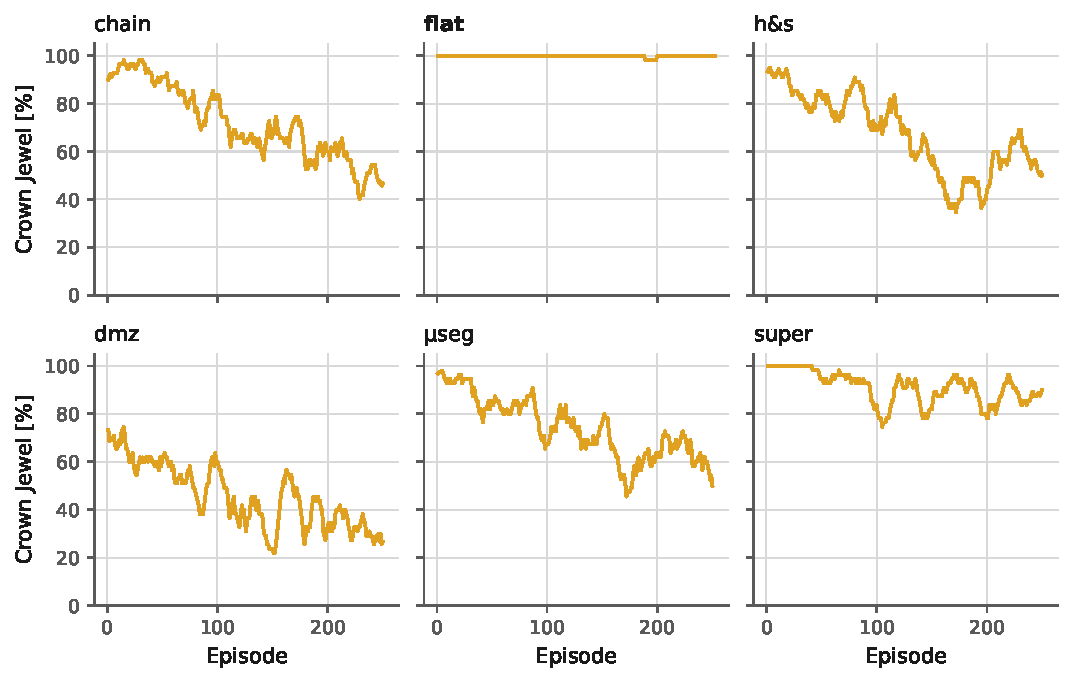
\includegraphics[width=\textwidth]{cj_flat}
  \caption[Crown-Jewel-Quote auf \emph{flat}]{Crown-Jewel-Quote der Verteidiger
  auf \emph{flat} gegen alle sechs Angreifer.}
  \label{fig:cj-flat}
\end{figure}

\begin{figure}[H]
  \centering
  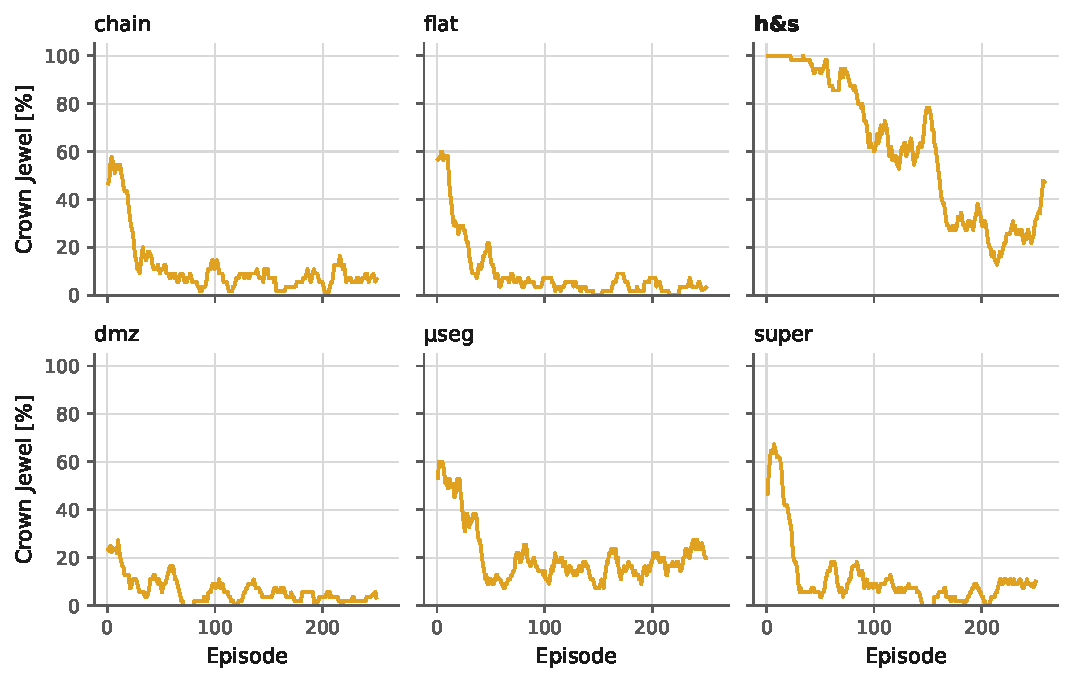
\includegraphics[width=\textwidth]{cj_hub_and_spoke}
  \caption[Crown-Jewel-Quote auf \emph{hub\_and\_spoke}]{Crown-Jewel-Quote der
  Verteidiger auf \emph{hub\_and\_spoke} gegen alle sechs Angreifer.}
  \label{fig:cj-hs}
\end{figure}

\begin{figure}[H]
  \centering
  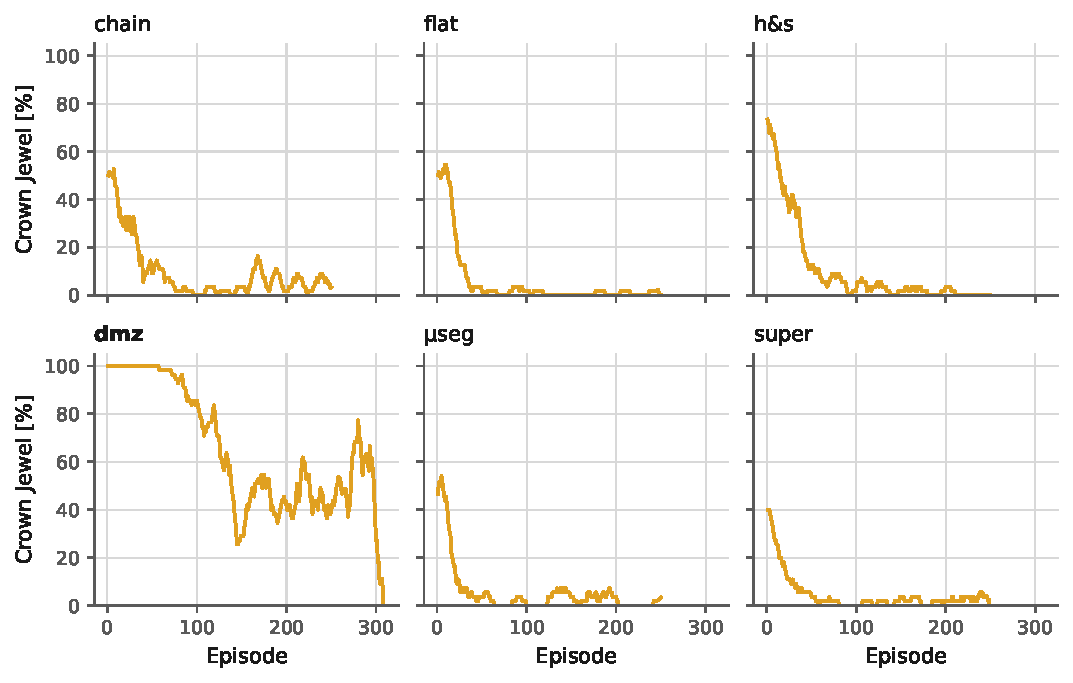
\includegraphics[width=\textwidth]{cj_dmz}
  \caption[Crown-Jewel-Quote auf \emph{dmz}]{Crown-Jewel-Quote der Verteidiger
  auf \emph{dmz} gegen alle sechs Angreifer.}
  \label{fig:cj-dmz}
\end{figure}

\begin{figure}[H]
  \centering
  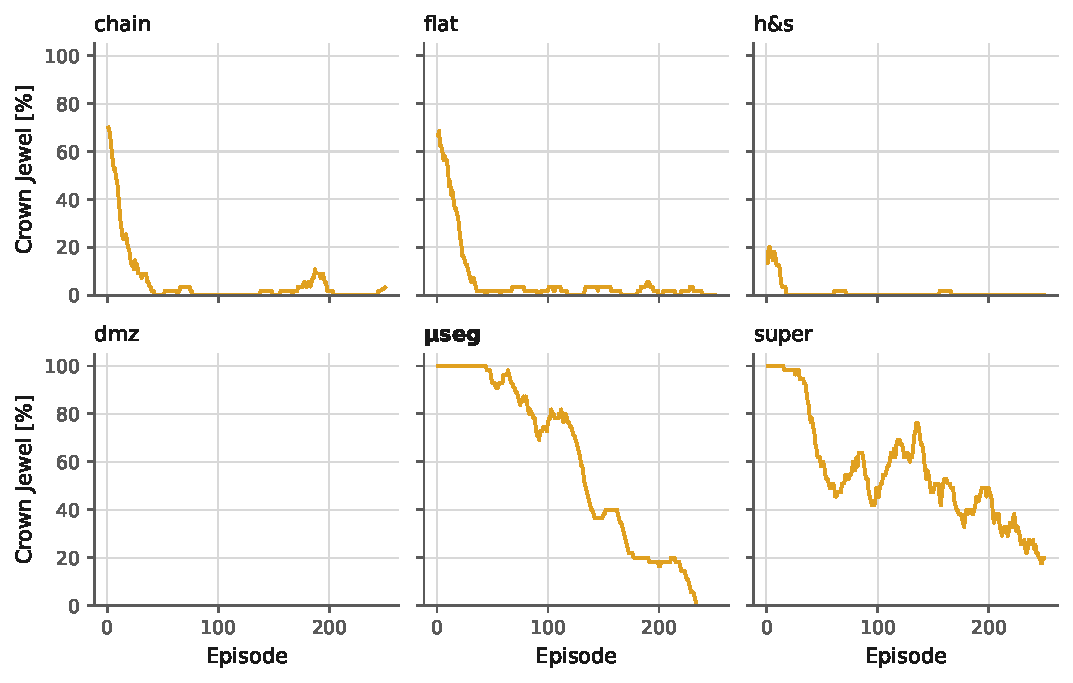
\includegraphics[width=\textwidth]{cj_micro_segmented}
  \caption[Crown-Jewel-Quote auf \emph{micro\_segmented}]{Crown-Jewel-Quote der
  Verteidiger auf \emph{micro\_segmented} gegen alle sechs Angreifer.}
  \label{fig:cj-ms}
\end{figure}

\section{Gehaltene Knoten je Topologie}
\label{app:knoten}

Die folgenden vier Abbildungen zeigen die größte Zahl gleichzeitig gehaltener
Knoten je Episode für alle 24 Matchups, gemittelt über die fünf Seeds und
geglättet über fünf Episoden. \Cref{sec:knoten-verlauf} stellt daraus nur
die vier Matchups auf der Diagonalen dar. Die Skala reicht in allen Feldern
von null bis zehn Knoten. Fett überschrieben ist jeweils das Feld des
Angreifers, der auf der verteidigten Topologie trainiert wurde.

\begin{figure}[H]
  \centering
  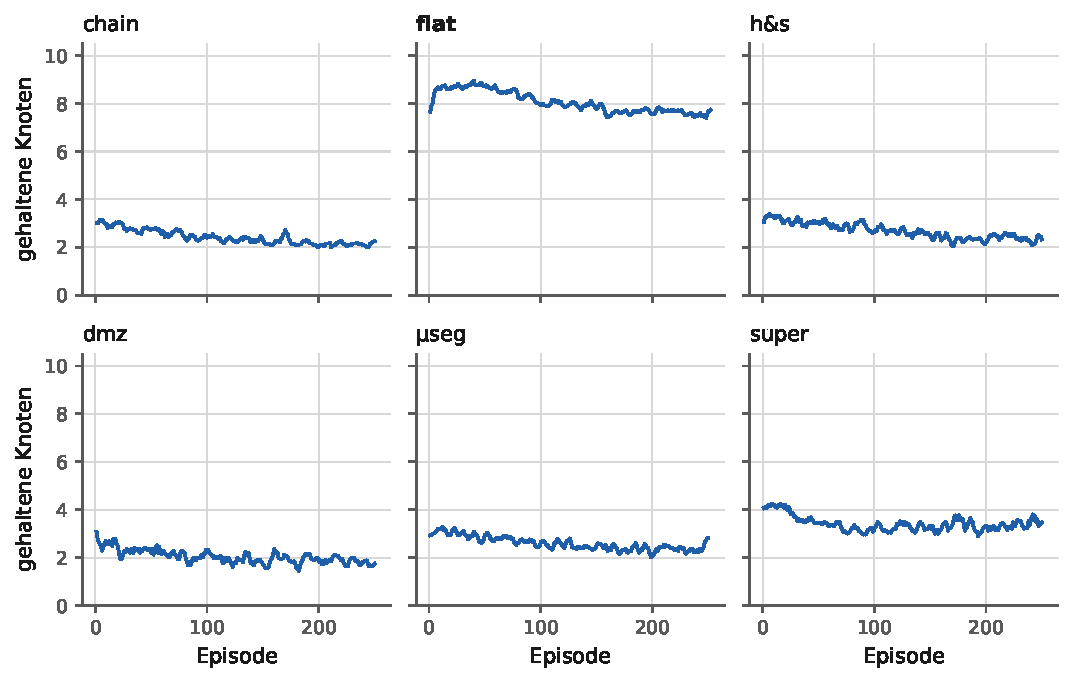
\includegraphics[width=\textwidth]{knoten_flat}
  \caption[Gehaltene Knoten auf \emph{flat}]{Gehaltene Knoten der Verteidiger
  auf \emph{flat} gegen alle sechs Angreifer.}
  \label{fig:knoten-flat}
\end{figure}

\begin{figure}[H]
  \centering
  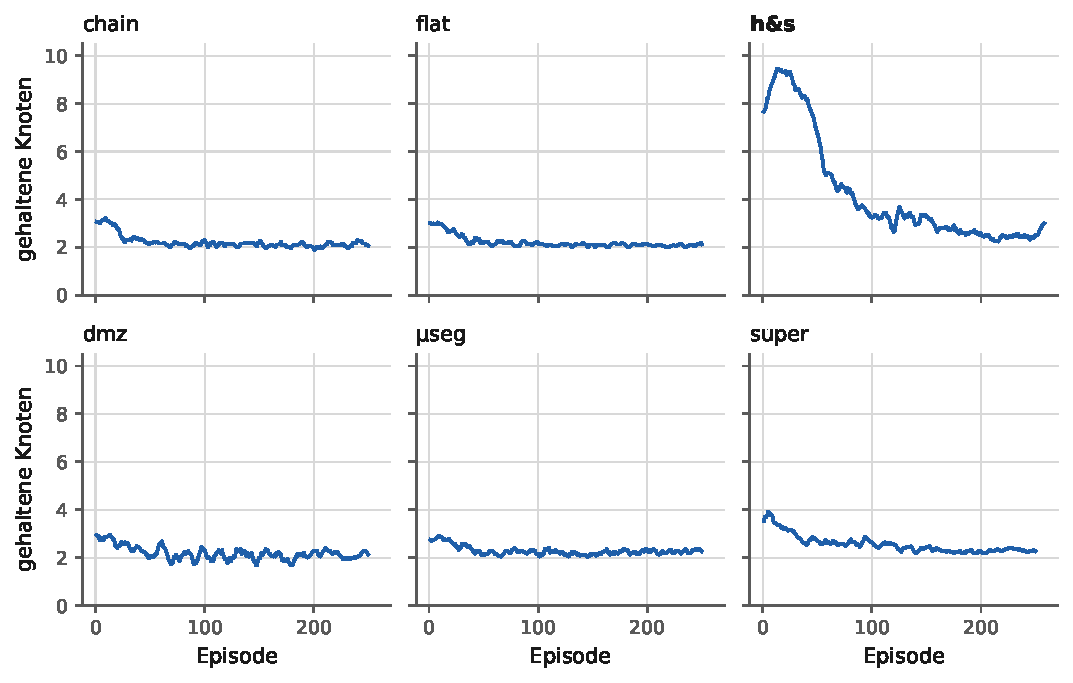
\includegraphics[width=\textwidth]{knoten_hub_and_spoke}
  \caption[Gehaltene Knoten auf \emph{hub\_and\_spoke}]{Gehaltene Knoten der Verteidiger
  auf \emph{hub\_and\_spoke} gegen alle sechs Angreifer.}
  \label{fig:knoten-hs}
\end{figure}

\begin{figure}[H]
  \centering
  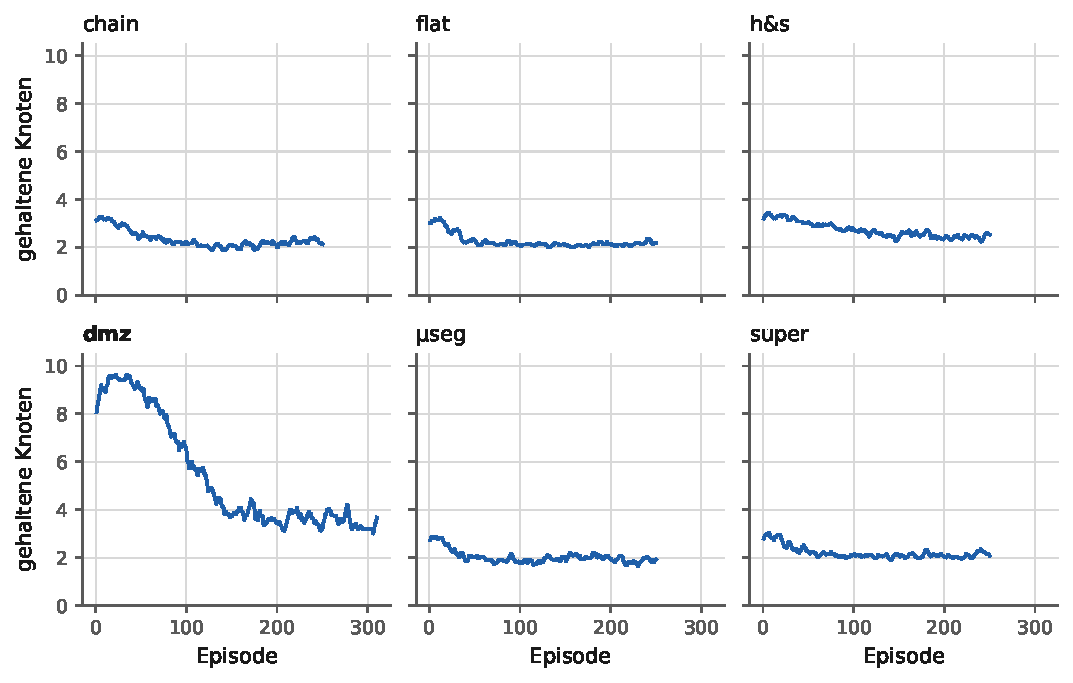
\includegraphics[width=\textwidth]{knoten_dmz}
  \caption[Gehaltene Knoten auf \emph{dmz}]{Gehaltene Knoten der Verteidiger
  auf \emph{dmz} gegen alle sechs Angreifer.}
  \label{fig:knoten-dmz}
\end{figure}

\begin{figure}[H]
  \centering
  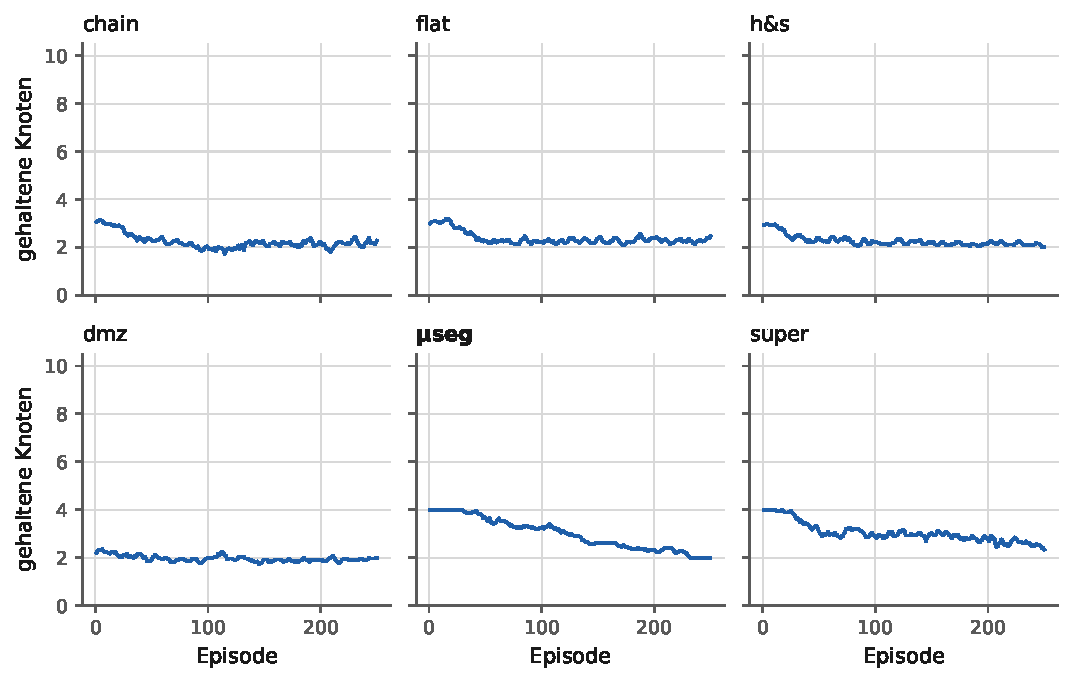
\includegraphics[width=\textwidth]{knoten_micro_segmented}
  \caption[Gehaltene Knoten auf \emph{micro\_segmented}]{Gehaltene Knoten der Verteidiger
  auf \emph{micro\_segmented} gegen alle sechs Angreifer.}
  \label{fig:knoten-ms}
\end{figure}

\section{\acs{SLA}-Brüche je Topologie}
\label{app:sla}

Die folgenden vier Abbildungen zeigen, in wie vielen Schritten je Episode die
Verfügbarkeit unter der Schwelle lag, gemittelt über die fünf Seeds. Jedes Feld
trägt eine eigene Skala, weil die Werte weit auseinanderliegen; $\Sigma$ nennt
die Summe aller Bruchschritte des Matchups über alle fünf Seeds.
\Cref{fig:sla-einbrueche} zeigt zwei dieser Fälle nach Seeds getrennt.

\begin{figure}[H]
  \centering
  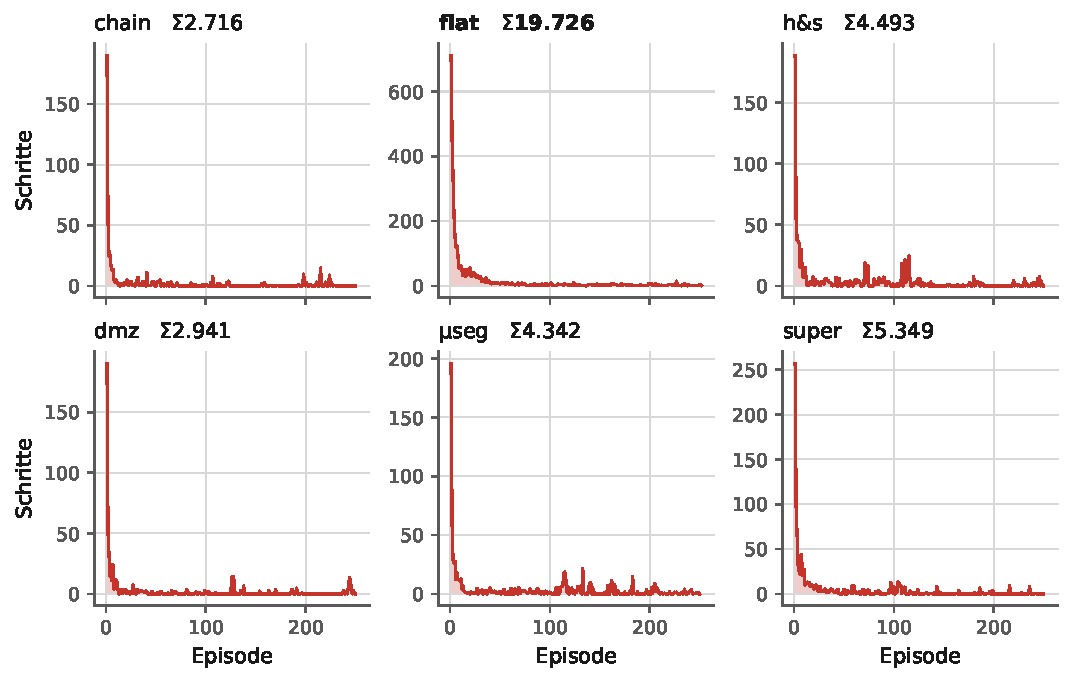
\includegraphics[width=\textwidth]{sla_flat}
  \caption[\acs{SLA}-Brüche auf \emph{flat}]{Schritte mit \ac{SLA}-Bruch der
  Verteidiger auf \emph{flat} gegen alle sechs Angreifer.}
  \label{fig:sla-flat}
\end{figure}

\begin{figure}[H]
  \centering
  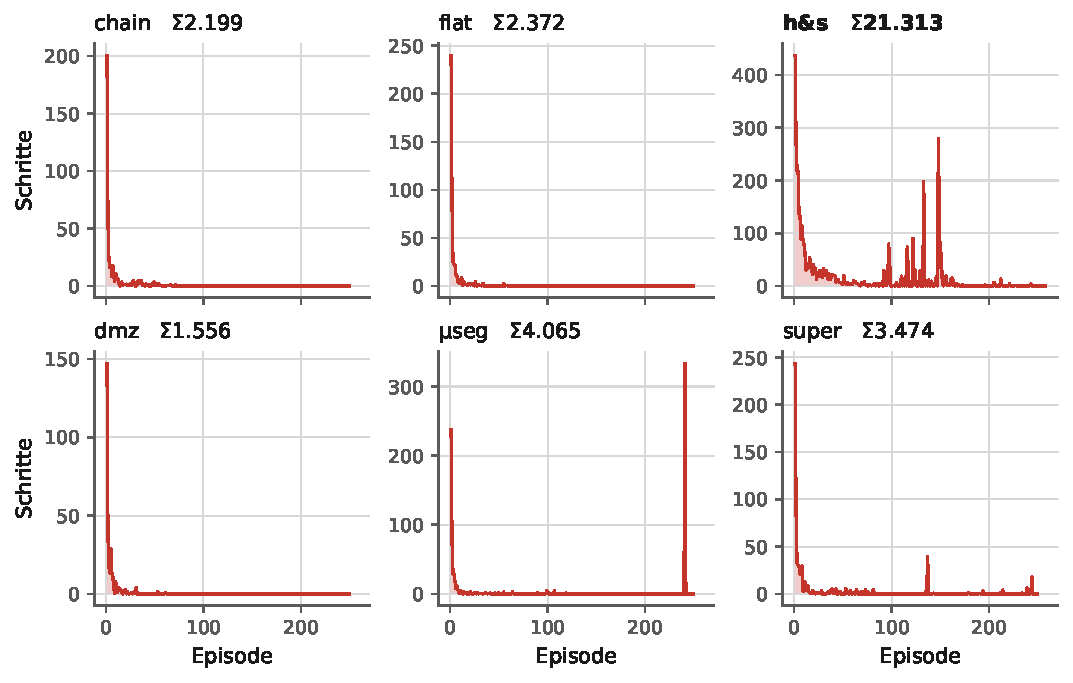
\includegraphics[width=\textwidth]{sla_hub_and_spoke}
  \caption[\acs{SLA}-Brüche auf \emph{hub\_and\_spoke}]{Schritte mit
  \ac{SLA}-Bruch der Verteidiger auf \emph{hub\_and\_spoke} gegen alle sechs
  Angreifer.}
  \label{fig:sla-hs}
\end{figure}

\begin{figure}[H]
  \centering
  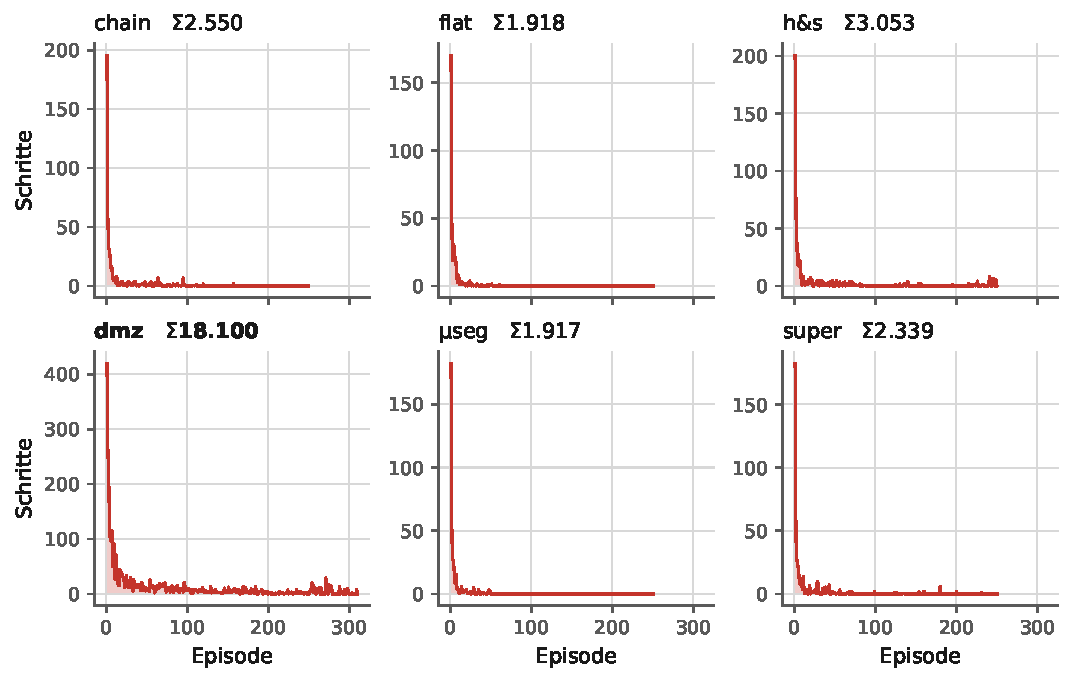
\includegraphics[width=\textwidth]{sla_dmz}
  \caption[\acs{SLA}-Brüche auf \emph{dmz}]{Schritte mit \ac{SLA}-Bruch der
  Verteidiger auf \emph{dmz} gegen alle sechs Angreifer.}
  \label{fig:sla-dmz}
\end{figure}

\begin{figure}[H]
  \centering
  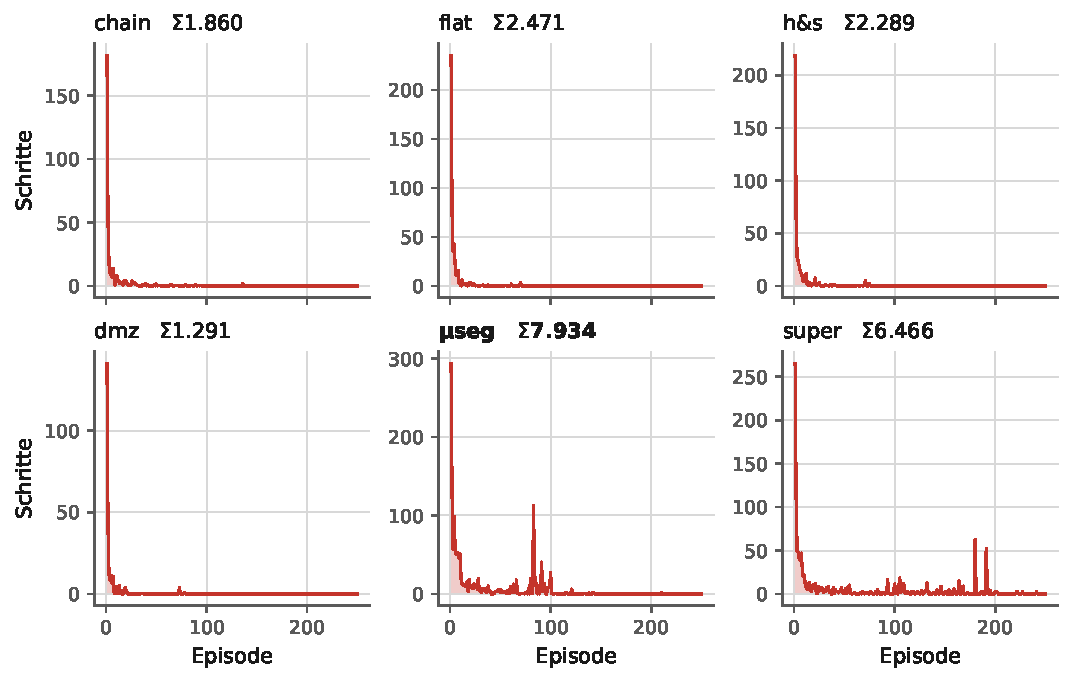
\includegraphics[width=\textwidth]{sla_micro_segmented}
  \caption[\acs{SLA}-Brüche auf \emph{micro\_segmented}]{Schritte mit
  \ac{SLA}-Bruch der Verteidiger auf \emph{micro\_segmented} gegen alle sechs
  Angreifer.}
  \label{fig:sla-ms}
\end{figure}


\section{Abwehrbonus je Topologie}
\label{app:abwehr}

Die folgenden vier Abbildungen zeigen den Abwehrbonus je Episode für alle 24
Matchups, gemittelt über die fünf Seeds und geglättet über fünf Episoden;
\Cref{sec:aktionen} zeigt daraus nur das Mittel über die sechs Angreifer je
Topologie. Die Skala ist in allen Feldern dieselbe, die Nulllinie ist
eingezeichnet. Fett überschrieben ist jeweils das Feld des Angreifers, der
auf der verteidigten Topologie trainiert wurde.

\begin{figure}[H]
  \centering
  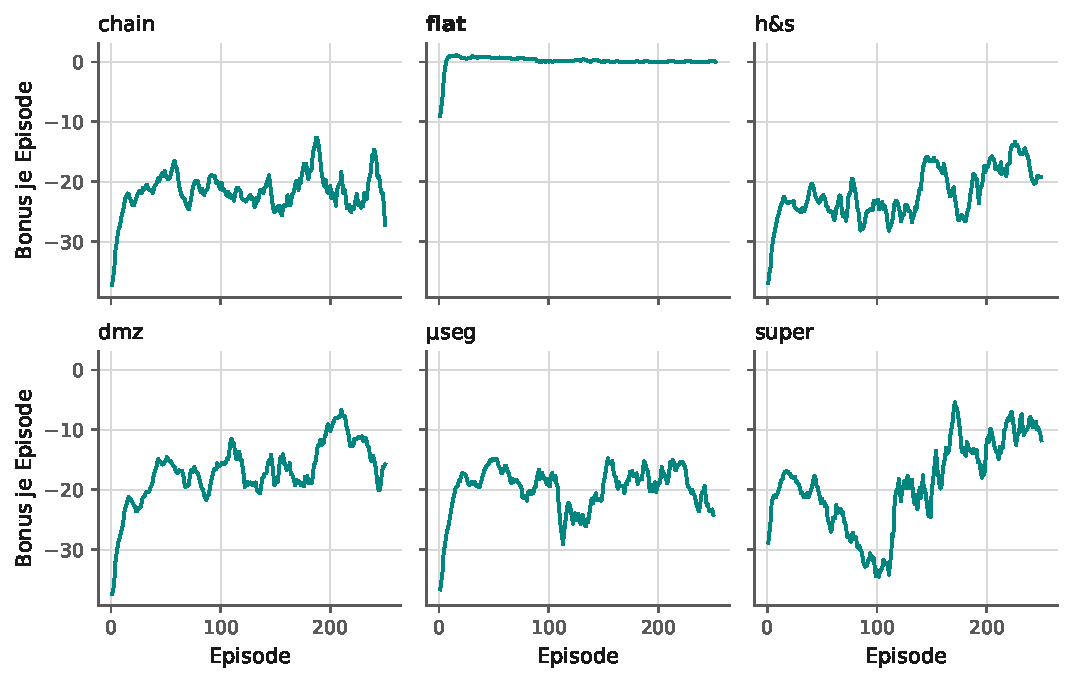
\includegraphics[width=\textwidth]{abwehr_flat}
  \caption[Abwehrbonus auf \emph{flat}]{Abwehrbonus der Verteidiger
  auf \emph{flat} gegen alle sechs Angreifer.}
  \label{fig:abwehr-flat}
\end{figure}

\begin{figure}[H]
  \centering
  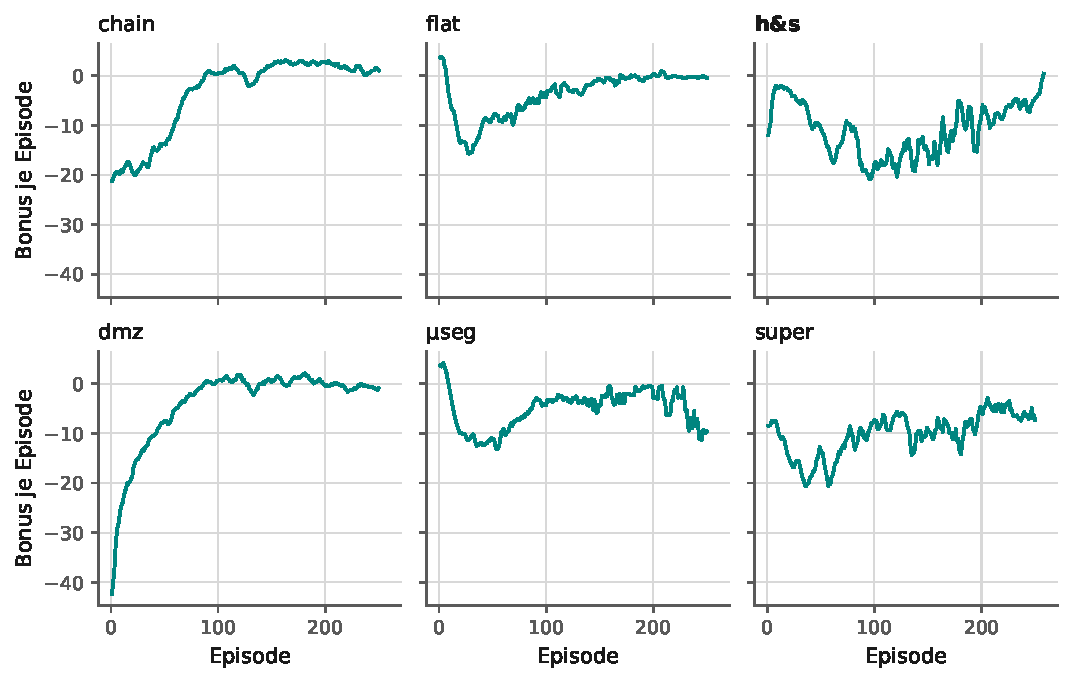
\includegraphics[width=\textwidth]{abwehr_hub_and_spoke}
  \caption[Abwehrbonus auf \emph{hub\_and\_spoke}]{Abwehrbonus der Verteidiger
  auf \emph{hub\_and\_spoke} gegen alle sechs Angreifer.}
  \label{fig:abwehr-hs}
\end{figure}

\begin{figure}[H]
  \centering
  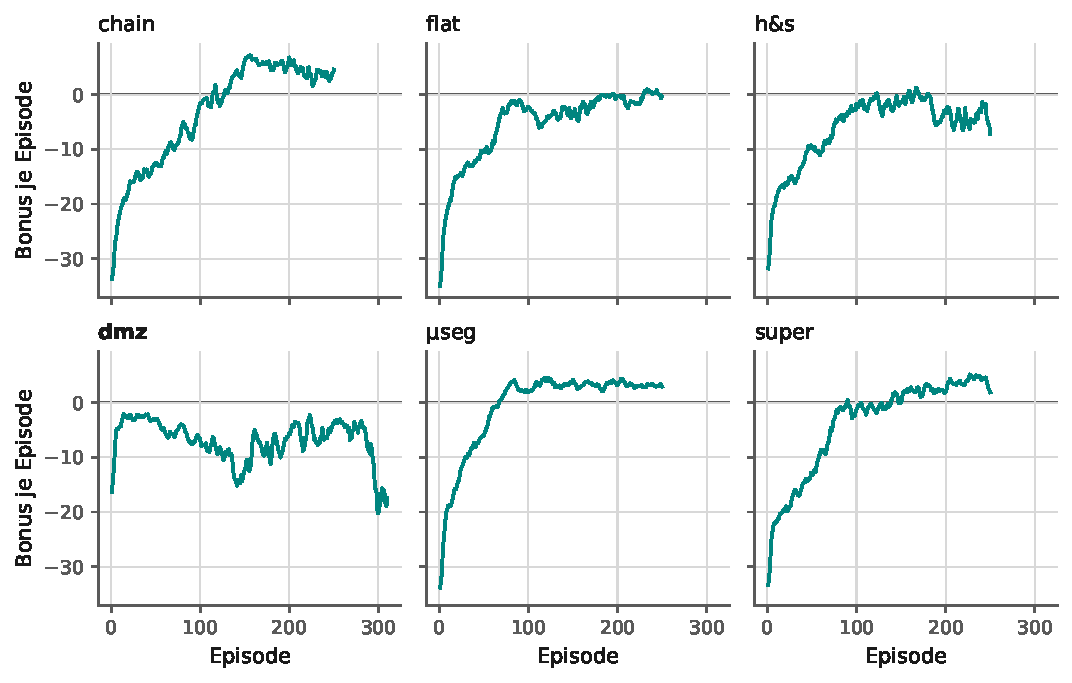
\includegraphics[width=\textwidth]{abwehr_dmz}
  \caption[Abwehrbonus auf \emph{dmz}]{Abwehrbonus der Verteidiger
  auf \emph{dmz} gegen alle sechs Angreifer.}
  \label{fig:abwehr-dmz}
\end{figure}

\begin{figure}[H]
  \centering
  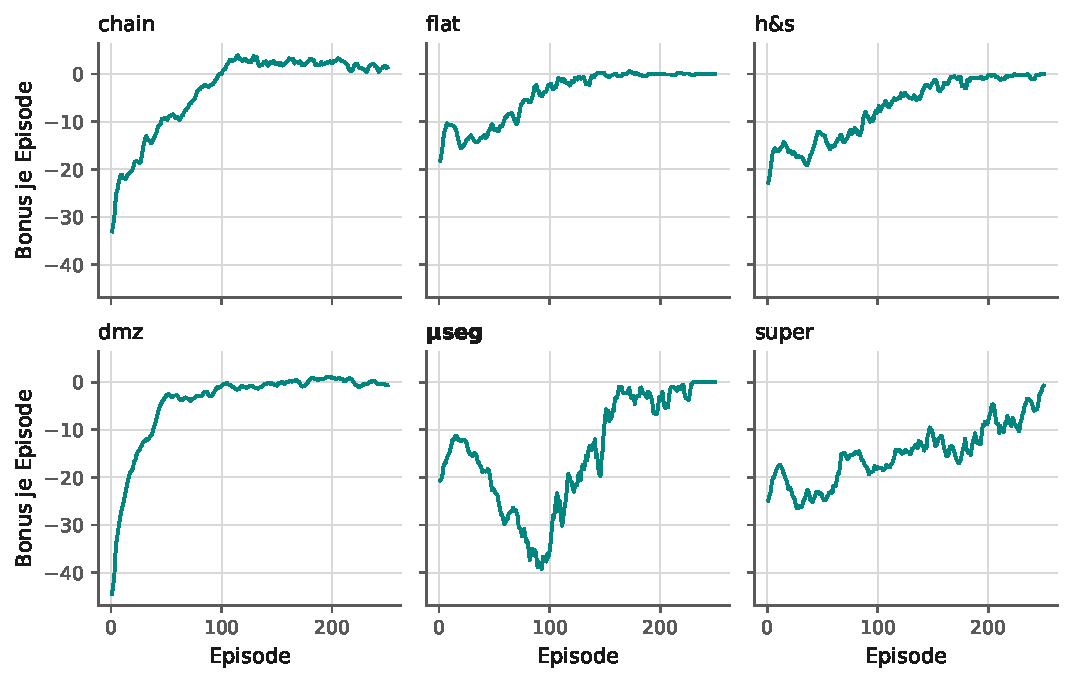
\includegraphics[width=\textwidth]{abwehr_micro_segmented}
  \caption[Abwehrbonus auf \emph{micro\_segmented}]{Abwehrbonus der Verteidiger
  auf \emph{micro\_segmented} gegen alle sechs Angreifer.}
  \label{fig:abwehr-ms}
\end{figure}

\section{Konvergenzmarken je Topologie}
\label{app:konvergenz}

Die folgenden vier Abbildungen zeigen für alle 24 Matchups, an welcher Stelle
des Verlaufs die beiden in \Cref{sec:konvergenzergebnis} verglichenen Maße
greifen. Gezeichnet ist der Verteidiger-Reward, gemittelt über die fünf Seeds
und geglättet über fünf Episoden. Die drei Senkrechten markieren das Kriterium
aus \Cref{sec:konvergenz}, dasselbe Kriterium mit dem strengeren Trendtest aus
\Cref{sec:konvergenzergebnis} und die 90-Prozent-Marke aus
\Cref{sec:limitationen}, jeweils gemittelt über die fünf Seeds. Fett überschrieben ist das Feld des Angreifers, der auf
der verteidigten Topologie trainiert wurde.

\begin{figure}[H]
  \centering
  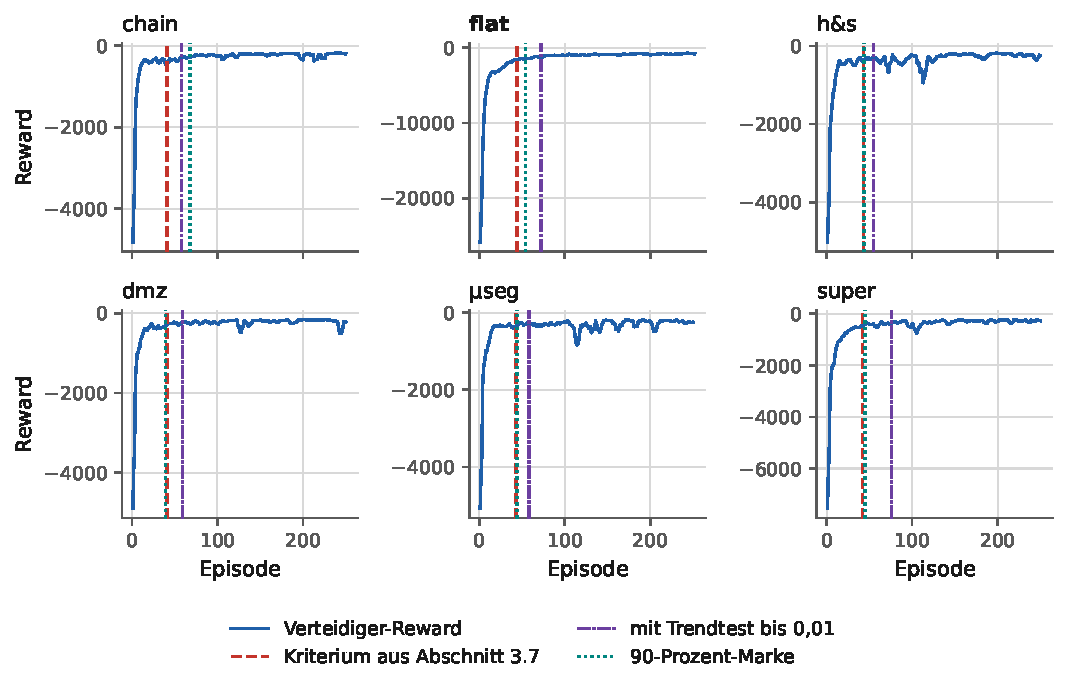
\includegraphics[width=\textwidth]{konvergenz_flat}
  \caption[Konvergenzmarken auf \emph{flat}]{Konvergenzmarken der Verteidiger
  auf \emph{flat} gegen alle sechs Angreifer.}
  \label{fig:konv-flat}
\end{figure}

\begin{figure}[H]
  \centering
  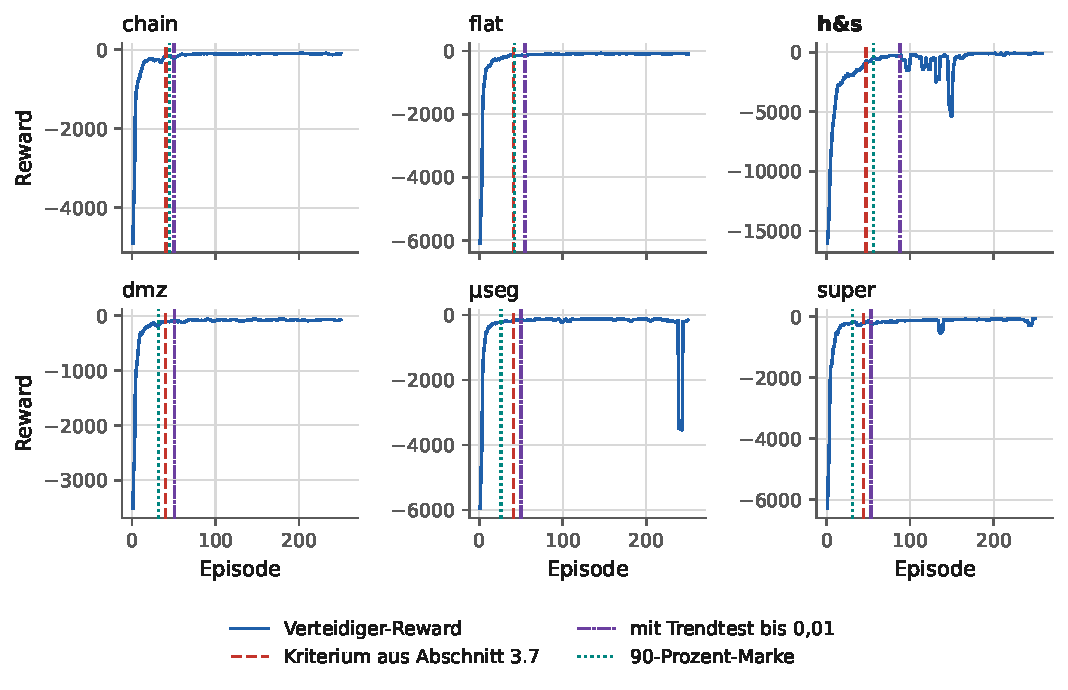
\includegraphics[width=\textwidth]{konvergenz_hub_and_spoke}
  \caption[Konvergenzmarken auf \emph{hub\_and\_spoke}]{Konvergenzmarken der
  Verteidiger auf \emph{hub\_and\_spoke} gegen alle sechs Angreifer.}
  \label{fig:konv-hs}
\end{figure}

\begin{figure}[H]
  \centering
  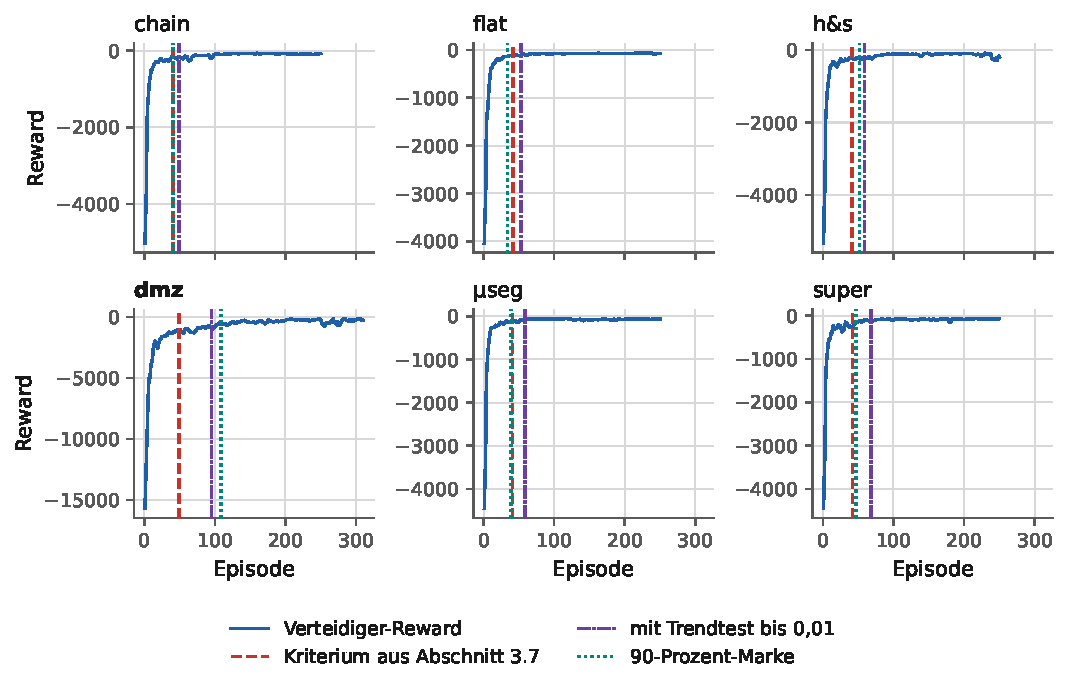
\includegraphics[width=\textwidth]{konvergenz_dmz}
  \caption[Konvergenzmarken auf \emph{dmz}]{Konvergenzmarken der Verteidiger
  auf \emph{dmz} gegen alle sechs Angreifer.}
  \label{fig:konv-dmz}
\end{figure}

\begin{figure}[H]
  \centering
  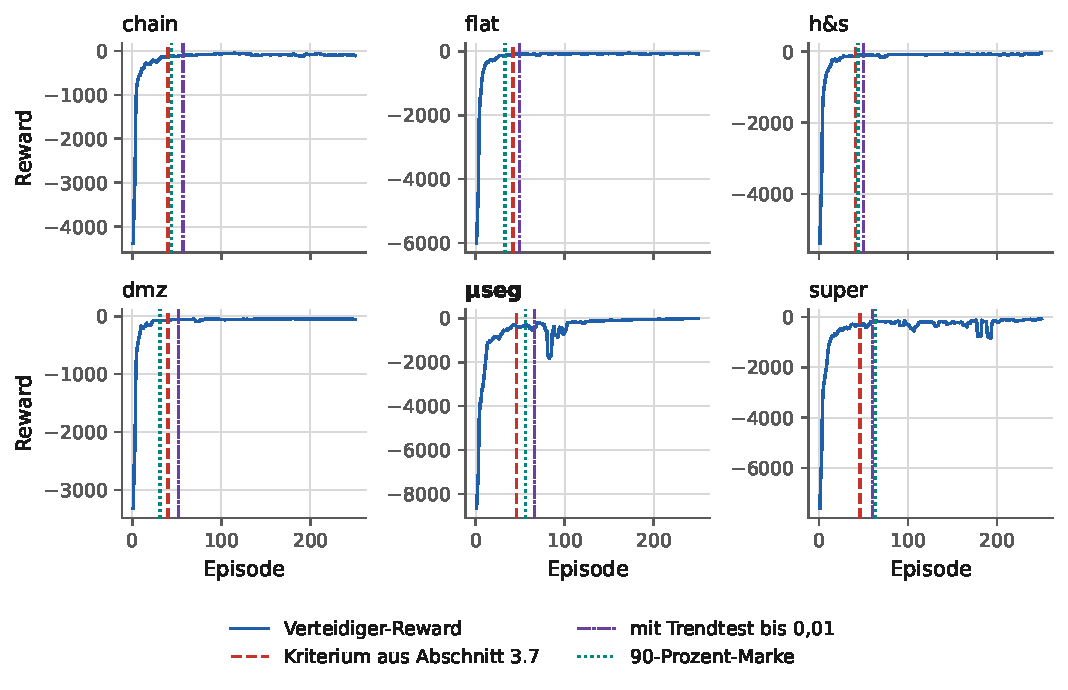
\includegraphics[width=\textwidth]{konvergenz_micro_segmented}
  \caption[Konvergenzmarken auf \emph{micro\_segmented}]{Konvergenzmarken der
  Verteidiger auf \emph{micro\_segmented} gegen alle sechs Angreifer.}
  \label{fig:konv-ms}
\end{figure}


% ── Eidesstattliche Erklaerung ───────────────────────────────────────
\cleardoublepage
% Eidesstattliche Erklärung
\chapter*{Eidesstattliche Erklärung}
\addcontentsline{toc}{chapter}{Eidesstattliche Erklärung}

Ich versichere an Eides statt, dass ich die vorliegende Bachelorarbeit
selbstständig und ohne fremde Hilfe verfasst und keine anderen als die
angegebenen Quellen und Hilfsmittel benutzt habe. Alle Stellen, die
wörtlich oder sinngemäß aus veröffentlichten oder nicht veröffentlichten
Schriften entnommen wurden, sind als solche kenntlich gemacht. Die Arbeit
hat in gleicher oder ähnlicher Form noch keiner Prüfungsbehörde vorgelegen.

Beim Anfertigen dieser Arbeit wurden KI-gestützte Werkzeuge eingesetzt: Claude
Code zur Unterstützung bei der Programmierung und bei der sprachlichen
Überarbeitung des Textes, Gemini Notebook zur Unterstützung bei der
Literaturrecherche. Sämtliche auf diesem Weg entstandenen Texte und
Programmteile habe ich geprüft und überarbeitet. Die Fragestellung, der
Versuchsaufbau sowie die Auswertung und Einordnung der Ergebnisse verantworte
ich; alle verwendeten Quellen sind im Literaturverzeichnis nachgewiesen und
wurden im Original geprüft.

\vspace{2cm}
\noindent
\begin{tabular}{@{}p{6cm}@{\hspace{2cm}}p{6cm}@{}}
  \hrulefill & \hrulefill \\
  Ort, Datum & Unterschrift \\
\end{tabular}


\end{document}
